\documentclass[a4paper]{book}
\usepackage[utf8]{inputenc}
\usepackage{amsmath}
\usepackage{amsfonts}
\usepackage{amssymb}
\usepackage{graphicx}
\usepackage{amsthm}
\author{Riste Gligorov}

\usepackage{multirow}
\usepackage{subfigure}
\usepackage{url}
\usepackage{booktabs}
\usepackage{epstopdf}
\usepackage[toc,page]{appendix}
\usepackage{float}

%\usepackage{abstract}
%\renewcommand{\abstractname}{}    % clear the title
%\renewcommand{\absnamepos}{empty} % originally center

\begin{document}

\tableofcontents

% table spacing
\newcommand\T{\rule{0pt}{3ex}}
\newcommand\B{\rule[-1.6ex]{0pt}{0pt}}

\newtheorem{thesisdef}{Definition}

\newcommand{\noop}[1]{} % a do-nothing command that serves a purpose

\chapter{Introduction}\label{chap:intro}

\begin{quotation}
\noindent 
In this chapter we introduce some of the motivating factors and the context of the research work presented in this thesis. We outline the three research questions this thesis is centered around and we describe the methods used to address them. We also present the related work and state the high-level contributions of the thesis.

This chapter is based on the paper entitled \textit{User-generated metadata in audio-visual collections} which was presented at the Doctoral Symposium of the 21st International World Wide Web Conference (WWW2012), held in Lyon, France.
\end{quotation}

\section{Context and Research Problems}
The central goal of this research work is to investigate the added value of user-generated metadata in professionals environments such as audio-visual archives. 
\subsection{Audio-visual Collections in the Digital Era}
Audio-visual (AV) content collections are undergoing a transformation from archives of analogue materials to very large stores of digital data accessible online. Prerequisite for successful information retrieval and collection management is quality metadata associated with collection items. Traditionally, the task of annotating video programs is strictly in the hands of professional cataloguers who adhere to well-established guidelines in the cataloguing process \cite{acrchivingphilosophy}. Usually, the resulting manually-crafted professional annotations are coarse-grained in a sense that they are referring to the entire program describing the prevalent topics. Fine-grained manual annotation of video fragments, on the other hand, is prohibitive, as the work involved is inevitably tedious, incomplete, and costly \cite{bouke}. However, a significant portion of user-content requests are targeted at video fragments rather than entire programs; a transaction-log analysis \cite{fragmentpercent} performed in a broadcast archive showed that fragment purchases account for 66\% of all purchases. As the program level professional annotations may be inadequate for locating or retrieving of fragments --- or any other task that involves fragments rather than entire programs --- the need for fine-grained annotations becomes clear. A possible solution to the problem of scarcity of fine-grained
 video metadata is to harness users' efforts to amass video fragment-level descriptions.
 
One of the most common forms of user-generated metadata are \textit{tags}. With the advent of the Web 2.0 the tagging phenomenon witnessed rapid proliferation in many
areas; image collections\footnote{http://www.flickr.com}, bookmark collections\footnote{http://www.delicious.com}, user video collections\footnote{http://www.youtube.com}. Experience has shown that joint efforts of user communities result in massive amounts of tags usually unparalleled --- in terms of quantity --- by what professionals can provide. Just to put things into perspective, in 200 years of existance the Library of Congress has applied their expert-maintained taxonomy to 20 million books\footnote{http://www.loc.gov/about/reports}, whereas, in only four years, Flickr's users applied their ad-hoc tagging vocabulary to over 25 million photos. This suggests that there is, indeed, a potential in engaging end-users in the video-annotation process. One way of achieving this is through so-called `games with a purpose' \cite{gwap}. To this end, the Netherlands Institute for Sound and Vision\footnote{http://portal.beeldengeluid.nl/} (S\&V) in cooperation with KRO broadcasting\footnote{http://www.kro.nl/} launched \textit{Waisda?} in May 2009, a multi-player video labeling game where players describe streaming video by entering tags and score points based on temporal tag agreements . The underlying assumption is that tags are probably valid --- trustworthily describe the video fragments --- if they are entered independently by at least two players within a given timeframe (see figure \ref{fig:waisda}). The motivation behind \textit{Waisda?} is to improve the access to S\&V collection~\cite{johanwebsci}. With \textit{Waisda?} the S\&V institute aims to collect metadata in a user vocabulary, as previous research \cite{Jorgensen2007} suggests that such metadata can help bridge the gap between the search queries and the indexing vocabulary. In addition, it is expected that the resulting time-related metadata of the content within the video can improve support for finding fragments within entire broadcasts~\cite{bouke}.

\begin{footnotesize}
\begin{figure}[t!]
\centering
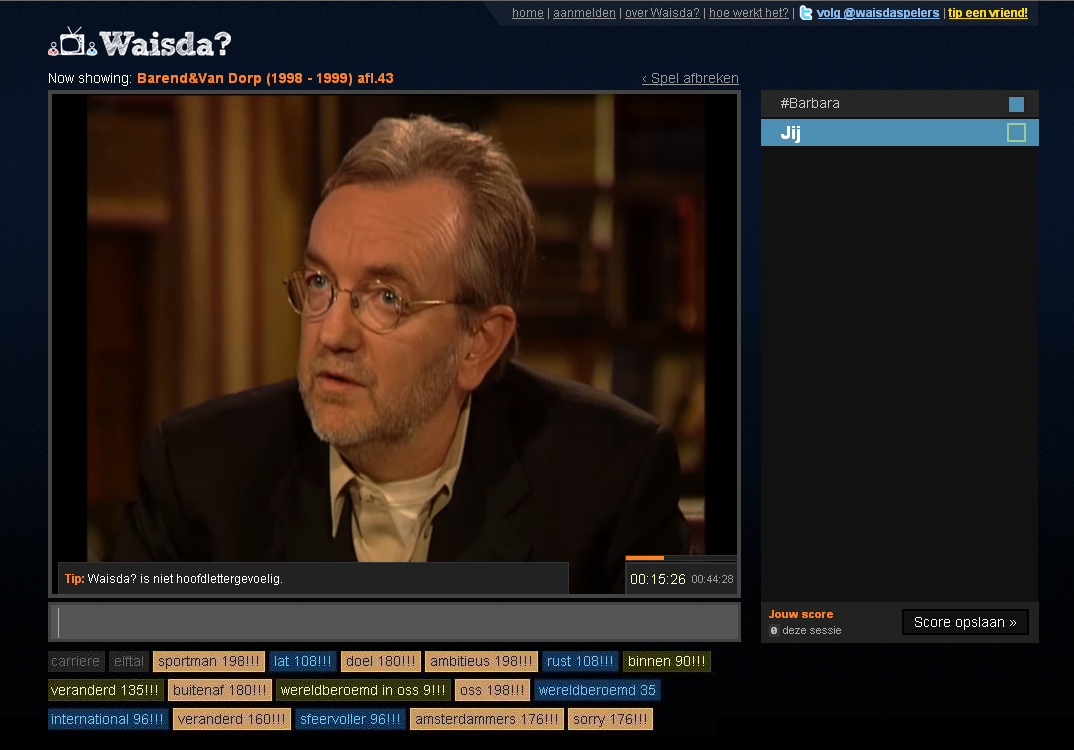
\includegraphics[scale=0.5]{intro:waisda_game}
\caption{Screenshot of the \textit{Waisda?} game interface: the central part of the screen is reserved for the video. Immediately below the tag input field and the list of tags entered already are placed. The coloration of the tags is indication of the number of points the tags scored.  On the right, there is the list of players currently in the game.}
\label{fig:waisda}
\end{figure}
\end{footnotesize}

\subsection{Project context}
This research is part of and funded by the \textit{PrestoPRIME}\footnote{http://www.prestoprime.org/} project which brings together various European audiovisual archives (including S\&V), research institutions, and industry partners. PrestoPRIME develops practical solutions for the long-term preservation of video and audio broadcasts, and finds ways to increase access by integrating the media archives with European on-line digital libraries. One of the considered ways to increase accessibility to videos is by exploiting user-generated tags collected through the labeling game \textit{Waisda?}.

\subsection{Research questions}\label{sec:research-questions}
The overall problem statement for this research is as follows.
\begin{quote}
\textit{What potential added value do user-generated video annotations have in professional environment?}
\end{quote}

To successfully integrate user-generated tags into AV collections' workflows a better understanding of their characteristics, compared to preexisting professionals annotations, is required. In particular,  the terminology that users employ when describing videos  and the aspects of the video that they usually describe. The first research question, therefore, is
\begin{itemize}
	\item[1.] What are the relationships between user-generated tags  and professional annotations in terms of the vocabulary and what they describe?
\end{itemize}
Locating a fragment within a video is an important use case in AV collections for which the fine-grained user tags could potentially provide an added value. Thus, the second research question addresses the usefulness aspect of user tags in terms of locating fragments within a video.
\begin{itemize}
	\item[2.] Can we improve fragment search  within video, with the help of user-generated data?
\end{itemize}
%Previous research \cite{websciencepaper,kcap,johanwebsci} has shown that user tags predominately describe objects and rarely refer to topics of a scene. Considering that professional annotations at scene-level are scarce, we investigate whether user tags can be used to deduce what the scene is about. Therefore, the third research question is
%\begin{itemize}
%	\item[3.] Can we derive topical description for scenes from user-generated tags?
%\end{itemize}

Lastly, successful integrations of user tags also requires that issues around assessing and improving tag quality to be addressed. The third and final research question, therefore, is
\begin{itemize}
	\item[3.] Can the quality of user-generated tags for videos be evaluated and improved?
\end{itemize}

\section{Related Work}
In this section we outline some of the related work. It should be noted that this is an incomplete list of the more relevant studies.
\subsection{Games With a Purpose}
Games with a purpose (or GWAPs) are computer games, in which people, as a side effect of playing, perform tasks computers are unable to perform \cite{gwap}. The first example of a GWAP was the ESP game \cite{CHI2004:vonAhn}, designed by Luis von Ahn, which harnesses human abilities to label images. %The game randomly pairs up two players with the task to describe images. When both players provide the same label for an image, they score points and proceed to the next image. The labels entered by both users are associated to the image as metadata. In other words, the consensus among users provides a method to ensure the quality and consistency of the labels. Evaluation shows that these labels can be used to retrieve images with high precision and are almost all considered as good descriptions in a manual assessment.
The idea to collect metadata through games with a purpose has been applied to video footage in, for example, the Yahoo! video tag game \cite{WWW08_vanZwol_etal},
VideoTag\footnote{http://www.videotag.co.uk/}, PopVideo\footnote{http://www.gwap.com/gwap/gamesPreview/popvideo/} and \textit{Waisda?}. Compared to the other video labeling games, \textit{Waisda?} is unique in the sense that it is initiated by an audiovisual institute (S\&V) with the purpose to improve the access to their collection~\cite{johanwebsci}.

\subsection{Evaluation of End-user Tags in Professional Environment}
The Steve project \cite{MATW2009:Leason} was one of first attempts to explore the role of user-generated metadata. In this collaboration of several art museums a collection of artworks was made available to the general public who were asked to tag them. Among other things, the project studied the relationship of the resulting folksonomy to professionally created museum documentation. The results showed that users tag the artworks of art from a perspective different than that of museum documentation: around 86\% of tags were not found in museum documentation.

Museum staff also assessed the tags from the steve.museum project on usefulness when used to search for artworks. From the total number of tags, 88.2\% were found to be useful. Following the methodology of steve-museum, S\&V institute also asked a senior cataloguer to judged a sample of \textit{Waisda?} tags on their usefulness when searching for videos \cite{johanwebsci}. The sample consisted of the 20 most frequent and the 20 least frequent tags from two television programs. The cataloguer found the majority of the tags to be useful. She also noted that there seems to exist a difference between professional descriptions and end-user tags. While professionals describe the topical subject of the program, the players in \textit{Waisda?} generally tag things that can be directly seen or heard in the video. One of the aims of this research is to investigate the characteristics of the tags and what they describe in the video more methodically, and on a larger scale.

\subsection{User annotations for search}
Search based on user-generated metadata, in particular folksonomies, has been studied before. Morrison compared web search performance of folksonomies from social bookmarking web sites against search engines and subject directories \cite{morison}, showing that search engines had the highest precision and recall rates. Folksonomies, however, performed surprisingly well. In fact, user tags show promise to alleviate the vocabulary mismatch problem for search: bridging the gap between user queries and metadata used for retrieval \cite{vocprob}. Indeed, Geisler and Burns state that YouTube tags provide added value for search, because 66\% of them do not appear in  other metadata \cite{youtube}. Heymann et al. investigated a large-scale sample of forty million bookmarks from the social bookmarking site del.icio.us and found that in 20\% of the cases user tags do not occur in the page text, backlink page text, or forward link page text of the pages they annotate. Studies in \cite{Bischoff:2010:BGT:1833903.1834001,Halvey:2007:AOV:1286240.1286301,journals/jasis/Rorissa10,Yanbe:2007:SBE:1255175.1255198} investigate this phenomenon across multiple domains and multimedia resource types and identify the gaps between the tag space and the querying vocabulary. The common conclusion is that user tags can improve search by bridging the vocabulary gap. 

Studies reported in \cite{Bischoff:2008:TUS:1458082.1458112,Sun:2010:QTR:1873951.1874029} take a more critical stance. They conclude that while overall user tags improve search, not all tags are suitable for retrieval. This hints that a characterization of the quality of the tags is needed to filter out the tags that are not suited for retrieval. This is one of the aspects that we address in this thesis. 

Another line of research is exploiting the tripartite structure ($Users \times Tags \times Resources$) of folksonomies to improve search \cite{Hotho:2006:IRF:2094613.2094652,Bao:2007:OWS:1242572.1242640}. Alternatively, the semantics of tags can be grounded in some lexical sources and the grounded tags utilized for improving search. For example, Hildebrand et al. proposed and investigated a semi-automatic process of assigning explicit meaning to user tags for video by linking them to concepts from the Linked Open Data cloud \cite{michiel}.

\subsection{Quality and Refinement of Annotations}
There is a substantial body of research into the refinement and quality assessment of annotations of still images. Lee at al. propose a tag refinement technique that aims at
differentiating noisy tag assignments from correct tag assignments \cite{Lee:2010:TRI:1890924.1891010}. Each tag is assigned a probability of being noisy based on the visual similarity of the images and tag co-occurrence statistics. Tags with a probability below a threshold are discarded as noisy. 

In \cite{Truong:2012:CSK:2324796.2324808,Li:2008:LTR:1460096.1460126} neighbour voting schemes for determining the tag relevance are explored. In this approach, a tag is considered more relevant to the image it is ascribed to, also known as the seed image, if the tag is also used to annotate the neighbouring images. The neighbourhood relation is defined in terms of the visual similarity among images. Lee at al. expand the approach by not only considering the visually similar images, but the dissimilar images as well, thus providing negative examples \cite{Lee:2012:TDE:2390876.2390880}. Kennedy at al. exploits visual similarity among images in a sense that tags ascribed to images by the creators of the image are used as seed annotations and also attached to visually similar images \cite{Kennedy:2009:RTU:1631135.1631139}. Zhao at al. propose a data-driven method to automatically determine the relatedness between a tag and the image's visual content taking into consideration the tag co-occurrence and the visual similarity among images \cite{Zhao:2010:TRV:2174490.2174571}.

Probabilistic methods that exploit random walk based techniques have also been explored \cite{Wang:2006:IAR:1180639.1180774,Liu:2009:TR:1526709.1526757,Li:2012:TRP:2382336.2382380}. These methods produce a ranking of the tags according to their relevance with respect to the image with which they are associated. The tag relevance estimations are computed as the stationary or the convergence probabilities of  a random walk processes. Notable example of this approach is the PageRank algorithm \cite{journals/corr/abs-1012-4872,10.4137/GRSB.S702,junker2008analysis}. Another group of methods exploit background knowledge (such as the lexical database Wordnet and a massive corpus indexed by Google) to perform the refinement of the image annotations \cite{Jin:2010:KBI:1731523.1731529,Wang:2007:RIA:1282280.1282343}. The semantic relations encoded in Wordnet and the semantic similarity quantified by the Google-based measures like the Normalized Google Distance \cite{DBLP:journals/corr/abs-cs-0412098} provide contextual evidence for the relationship among the annotations. This evidence is then used as an input for machine learning algorithms which give the final word for the quality of the annotations.

\section{Approach}
In this section we outline the approach to answer the research questions stated above. The specific approach for each of the research questions is described in separate subsection. The order of the subsections is respective to the order in which the research questions are stated in section \ref{sec:research-questions}. At the basis of each of the approaches lies \textit{Waisda?} which was used as a data-collection tool. In the course of this thesis significant effort went into improving the game design and development of software extension that enables seamless integration of the game into larger workflows. Chapter \ref{chap:waisda} describes the game in more detail and outlines the contributions of this thesis with respect to the development of the game.

\subsection{\textit{Waisda?} User Tags vs. Professional Annotations}\label{sec:user-professional}
To answer the first research question `What are the relationships between user-generated tags  and professional annotations in terms of the vocabulary and what they describe?' we perform two studies. Details can be found in \cite{websciencepaper,kcap}.

The first study is a quantitative data analysis of the entire tag collection gathered with \textit{Waisda?} during the first six months after the game was deployed. In order to estimate the lower bound of the fraction of user tags that are meaningful words, we examine the overlap between them and general lexical resources and vocabularies. Furthermore, to determine if users and professionals use different vocabularies when describing videos, we investigate the overlap between all user tags and a typical domain thesaurus used by professionals in the cataloging process. The results from the study show that there is, indeed, a terminological gap between users and professionals; while approximately 89\% of all user tags are meaningful words only 8\% of them were found in the domain thesaurus used by professionals.

In the second study, we take a combined approach. First, we investigate what do users tend to describe  more: things \textit{heard} or things \textit{seen} on screen. To this end, we perform a study on the overlap between the user tags and the audio signal --- subtitles for hearing impaired persons --- for a sample of episodes. Second, to get a more comprehensive understanding of the types of tags users usually add, we perform a qualitative study of a sample of user tags obtained through the \textit{Waisda?} video tagging game. In particular, each tag from the sample is manually analyzed in the light of the video content it describes and categorized in terms of the Panofsky-Shatford classification framework. The results of the study show that user tags predominately describe objects and rarely refer to topics of a scene. This is in sharp contrast with the professional annotations which  exclusively target the topic(s) of the entire video and (lot less frequently) of particular scenes. 


\subsection{Investigating the Added-value of User Tags for Fragment Search}\label{sec:fragment-search}
Fragment search within video is widely recognized as an application scenario of particular business importance in the AV collections world \cite{fragmentpercent}. However, the existing professional annotations generally refer to the entire video and are not tied to a specific time-point, which decreases their usefulness for fragment retrieval; without temporal data one needs to manually locate the fragment of interest. \textit{Waisda?} tags, on the other hand, do refer to fragments and are time-based, with time codes that \textit{deep link} to particular point in the video. Our aim is to investigate their added-value for fragment retrieval. Furthermore, we plan to explore what kind of query tasks (search for \textit{events}, \textit{objects}, etc.)  benefit from the user tags.

The methodology that we consider is \textit{quantitative system evaluation} \cite{vorhees}. In order to evaluate effectiveness of information retrieval, this methodology requires collection of ``documents'' (in our case video fragments), set of queries, and relevance judgments  indicating which ``documents'' in the collection should be returned for each query. We plan to create evaluation dataset from the videos that were part of \textit{Waisda?} game deployment and tagged by players. For such a dataset real-life, authentic user tags would already be available. However, set of fragments, relevance judgements, set of queries and query task types need to be defined. The method of achieving this is going to be part of and one of the contributions of the research.
	
An alternative is to creating an evaluation dataset is using an existing one. There are various video retrieval evaluation initiatives like TRECVID\footnote{http://trecvid.nist.gov/} that provide datasets for testing content-based retrieval techniques. The advantages of reusing such a dataset are (i) the set of fragments is defined, (ii) the set of queries and the relevance judgments are defined. The drawbacks are that \textit{Waisda?} like games have not been run yet on this dataset and setting up such a game and attracting sufficient users for this material could turn out to be hard. Also we are limited to the query task types defined by the dataset. Our position is that the effort required to collect user tags for the material outweighs the advantages offered by this approach.
	


%\subsection{Deriving Topical Descriptions From User Tags}\label{sec:topical-desc}
%Video fragments or scenes are often multivalent in terms of their meaning and as such can be observed as a mixture of topics. User tags collected through \textit{Waisda?}, which are mostly referring to objects, can be seen as instantiations of these topics. The challenge that we are facing is to derive topical descriptions from the user tags. The unstructured nature of the tags, --- only weak temporal ordering of tags within video exists, based on the tag entry time --- makes statistical approaches excellent candidates  for this task. The research we have done so far puts statistical \textit{topic models} at the top of the list. Topic models \cite{Hofmann, Blei} are a type of statistical models for discovering abstract `topics' in collection of documents. One of the most common topic models currently in use is the  Latent Dirichlet Allocationc (LDA). The idea behind LDA is to model documents as arising from multiple topics, where a topic is defined to be a distribution over a fixed vocabulary of terms. Specifically, it is assumed that $\mathit{K}$ topics are associated with a collection, and that each document exhibits these topics with different proportions. Furthermore, LDA assumes that words are exchangeable within each document, i.e., their order does not affect their probability under the model. In other words, each document is treated as a `bag of words'. We believe that the assumptions underlying the LDA model are valid in and applicable to our context as well. \textit{Videos} and \textit{scenes within videos}, much like documents, have many layers of meaning and can be viewed as mixture of topics. The high-level professional \textit{topical} descriptions, on the other hand, can be considered as the analog to topics in LDA. The low-level user tags are referring to things heard or seen on screen and as such can be viewed as instantiations of the particular topics the video/scene is about. The unstructured and unordered nature of user tags --- in the borders of a particular shot/scene --- fits the 'bag of words' metaphor quite well. Regardless of the choice of the method the procedure we envision will proceed in four steps.

%\begin{enumerate}
%	\item \textit{Video segmentation}. Videos are segmented into shots (possibly scenes) using state of the art video analysis tools.
%	\item \textit{Tag-to-Shot association}. Tags are associated to the shots (scenes) derived in the first step. In this process the temporal information associated to each tag will be used and special attention will be payed to user tags assigned close to the detected boundaries.
%	\item \textit{Model training}. Statistical model is trained. The collection of topics used by the professional catalogers from the Sound and Vision Institute will be used as a list of abstract topics. We consider this set to be a representable and relevant for two reasons. (1) The videos that will be considered will originate from their catalogue. (2) Every single topical description in their catalog comes from this set. As a training corpus we shall use the Sound and Vision cataloque: each cataloque entry is annotated with topical descriptors and is associated to contextual documents that contain textual description of the program's content. Additional corpora may be used as well.
%	\item \textit{Topics inference}. Using the trained model, for each shot (scene), the most probable  topics will be inferred from the tags associated to it.
%\end{enumerate}

%We plan to evaluate the effect that the inferred topical descriptions will have on fragment retrieval. For this we will use the test data set from the fragment retrieval study described in section \ref{sec:fragment-search}.

\subsection{User Tag Quality Metrics}\label{sec:quality}
Our supposition is that any characterization of quality of the user tags is largely determined by how different institutions will use them. In other words, it is immaterial to talk about tag quality without a specific application scenario in mind. Fragment search within video is widely recognized as an application scenario of particular business importance in the AV collections world. For these reasons, our characterization(s) of tag quality will be limited to this scenario.  Some of the aspects we plan to investigate in the context of the retrieval scenario are tag frequency and discriminative power of tags,  correlation between reputation of players and tag relevance,  semantic ambiguity of tags, overlap with transcripts,  etc. The exact specifics of this study will be determined by the outcome of the previous studies. Therefore, we plan to make the choice of research methodology and the type of output (e.g. quantitative metrics or set of recommendations) this study will provide after the fragment retrieval study is performed.

\section{Structure of the Thesis}
The thesis is organized as follows. In Chapter 2 we study the characteristics of the tags collected with \textit{Waisda?}. In particular, we focus on two aspects. First, what is the relationship between the game  tags and the annotations created by professional catalogers. Second, we investigate which facets of the video content are typically targeted by the game tags and at what level of semantic specificity. In the following two chapters we study the effectiveness of game tags for video retrieval by addressing two prominent search scenario that arise in practice. In Chapter 3 we look into the first scenario which is retrieving videos that feature visual appearances of given objects of interest. In Chapter 4 we focus on the second scenario which is topical search, retrieval of videos that are about a given topic. In Chapter 5 we outline the technical specifications of \textit{Waisda?} and address two important points. First, how can \textit{Waisda?} be deployed and used by audio-visual collection owners to tag their collection. Second, how can \textit{Waisda?} be integrated into larger systems and workflows. Lastly, in Chapter 6 we present the overall conclusions of this thesis. We discuss the implications of this work and suggest directions for future research. 

\section{Publications}
Publications on which the chapters of this thesis are based:
\begin{itemize}
	\item Chapter 1 was published as: Riste Gligorov. User-generated metadata in audio-visual collections. In the \textit{Proceedings of the 21st international conference companion on World Wide Web (WWW 2012), Lyon, France, 2012.}
	\item Chapter 2 was published as: Riste Gligorov, Michiel Hildebrand, Jacco van Ossenbruggen, Guus Schreiber, and Lora Aroyo. On the role of user-generated metadata in audio visual collections. In the \textit{Proceedings of the International Conference on Knowledge Capture (K-CAP 2011)}, pages 145-151. ACM Press, June 2011.
	\item Chapter 3 was published as: Riste Gligorov, Michiel Hildebrand, Jacco Van Ossenbruggen, Lora Aroyo, and Guus Schreiber. An Evaluation of Labelling-Game Data for Video Retrieval. In \textit{Advances in Information Retrieval: 35th European Conference on IR Research (ECIR 2013)}, pages 50-61, Springer, Moscow, Russia, March 2013.
	\item Chapter 4 is an extension of: Riste Gligorov, Michiel Hildebrand, Jacco Van Ossenbruggen, Lora Aroyo, and Guus Schreiber. Topical Video Search: Analysing Video Concept Annotation through Crowdsourcing Games. In the \textit{International Journal of Human Computation 4(1)}, 47-66, 2017.
	\item Chapter 5 is an extension of: Michiel Hildebrand, Maarten Brinkerink, Riste Gligorov, Martijn Van Steenbergen, Johan Huijkman, and Johan Oomen. \textit{Waisda?}: video labeling game. In the \textit{Proceedings of the 21st ACM international conference on Multimedia}, pages 823-826, Barcelona, Spain, 2013. This publication describes the technical aspects of the game and the main author is Michiel Hildebrand. Chapter 5 incorporates the content of the publication and additionally, describes the contribution of the work carried out for this thesis on design and implementation of the game. 
	
\end{itemize}

\section{Contributions}
The main contributions of the thesis are:
\begin{itemize}
\item A method to analyze quantitatively the overlap between user and professional terminology exploited in video annotation.
\item Qualitative analysis of the aspects of the video content which are described by the game tags i.e. \textit{what do game tags describe in a video and how}.
\item A method to design a dataset ---including fragments, queries, and relevance judgements --- for evaluating the added value of user tags for \textit{visual} and \textit{topical} video search.
\item Two evaluation datasets ---one for visual and one for topical search --- which contain fragments, user tags from \textit{Waisda?} collection, queries, and relevance judgements.
\item Quantitative evaluation of the added value of the game tags in terms of \textit{visual} and \textit{topical} video search.

\item A method for qualitative analysis/classification of the search results in the context of visual search. The aim of the analysis was to discover the types of tags that are generally responsible for false positives.

\item Qualitative analysis of the search results in the context of topical search. The aim of the analysis was to discover tagging practices that generally produce relevant topical tags.

\item Evaluation of tag-related measures for accessing the quality of the game tags as topical descriptors in the context of topical video search.

\item Development of extension module for \textit{Waisda?} which enables integration of the game in AV collection workflows. The module is part of the latest release of \textit{Waisda?} which is available online\footnote{The \textit{Waisda?} source code and documentation is available from Github \url{http://github.com/beeldengeluid/waisda}}.
\end{itemize}



\chapter{Game Tags in Audio Visual Collections}\label{chap:kcap}
\begin{quotation}
\noindent
In this chapter we study the characteristics of the user tags collected with the video labelling game \textit{Waisda?}. We address two aspects related to the user tags. First, we investigate to what extent does the terminology employed by the users when tagging videos differ from the terminology used by the professional cataloguers. Second, we examine which facets (\textit{who}, \textit{what}, \textit{where}, and \textit{when}) of the videos tagged by the users are typically described by the user tags and what is the level of specificness (\textit{abstract}, \textit{general}, and \textit{specific}) of the said tags. 
The findings in this chapter outline some of the strengths but also the limitations of the user tags. Our analysis shows that there is a terminological gap between the players of \textit{Waisda?} and the professionals. This makes the user tags a valuable asset as they are \textit{from the users and for the users} and can improve the access to the videos in the case when the ones accessing are the users themselves. Furthermore,  we find that user tags predominately describe instances (objects) in the video and rarely scenes. 
This fact hints that user tags could be useful for instance search and not so useful for topical search. These matters are addressed in the following chapters.

This chapter was published as ``On the Role of User-generated Metadata in Audio Visual Collections" in the Proceedings of the International Conference on Knowledge Capture 2011 \cite{kcap}. It was co-authored with Michiel Hildebrand, Jacco van Ossenbruggen, Lora Aroyo, and Guus Schreiber. 
\end{quotation}

\section{Introduction}

Crowdsourcing has gained attention as a method to collect large numbers of
metadata descriptions for media
objects~\cite{MATW2007:Chan,MATW2009:Leason,FlickrCommons}. Based on the idea
coined by Luis von Ahn~\cite{gwap}, a specific type of crowdsourcing has
become known as Games With A Purpose (GWAP). Inspired by this idea, the
Netherlands Institute for Sound and Vision deployed the video labeling game,
\emph{Waisda?}. Unique for this initiative is that the institute
aims~\cite{johanwebsci} to integrate the game into their workflow to
complement professional cataloguing and content based retrieval
techniques~\cite{ISR2009:hollink}. More specific, with \emph{Waisda?} they aim
to collect metadata in a user vocabulary that describes the content within the
video.

We investigate to what extent the aims of Sound and Vision are fulfilled by
analyzing the 420,000 user tags collected during the first pilot with
\emph{Waisda?}. To determine the vocabulary used by the crowd, we compare the
tags with existing controlled vocabularies. We compare the tags with the
professional metadata by matching them to terms of the institutes' in-house
thesaurus. Additionally, by matching the tags to the terms of a Dutch
linguistic database, we conclude that a large part of the tags are Dutch words
not used by professionals. To determine the type of content that the tags
describe we first compare them with the subtitles. Finally, we manually
classify the tags from a small number of videos. Using an existing
classification model, we show the relation between the content in the video
that is described and the type of tags that are used for these descriptions.

The rest of the paper is structured as follows. Section \ref{sec:related_work}
discusses related work. Section \ref{kcap:sec:approach} presents the approach we
take in tackling the goals we set forth. Section \ref{kcap:sec:materials} describes
the materials we used in our study. Section \ref{sec:experiments} reports on
the various experiments we performed on the user tags. Finally, section
\ref{sec:discussion} draws conclusions and points to some further directions
for research.

\newpage

\section{Related work}
\label{sec:related_work}

\subsection{Games with a purpose}

Games with a purpose (or GWAPs) are computer games, in which people, as a side
effect of playing, perform tasks computers are unable to perform \cite{gwap}.
The first example of a GWAP was the ESP game \cite{CHI2004:vonAhn}, designed
by Luis von Ahn, which harnesses human abilities to label images. The game
randomly pairs up two players with the task to describe images. When both
players provide the same label for an image, they score points and proceed to
the next image. The labels entered by both users are associated to the image
as metadata. In other words, the consensus among users provides a method to
ensure the quality and consistency of the labels. Evaluation shows that these
labels can be used to retrieve images with high precision and are almost all
considered as good descriptions in a manual assessment.

The idea to collect metadata through games with a purpose has been applied to
video footage in, for example, the Yahoo! video tag game
\cite{WWW08_vanZwol_etal},
VideoTag\footnote{\url{http://www.videotag.co.uk/}},
PopVideo\footnote{\url{http://www.gwap.com/gwap/gamesPreview/popvideo/}} and
\emph{Waisda?}. The gameplay of these video labeling games differs from the
ESP game in two ways: (i) multiple users can participate in a single game, and
(ii) the users score points when the same tag is entered in a specific time
interval. The underlying assumption is that tags are probably valid ---
trustworthily describe the video fragments --- if they are entered
independently by at least two players within a given time-frame. From here on
we shall refer to tags that are mutually agreed on as \textit{verified} tags.

Compared to the other video labeling games, \emph{Waisda?} is unique in the
sense that it is initiated by an audiovisual institute with the purpose to
improve access to their collection~\cite{johanwebsci}. With \emph{Waisda?} the
Netherlands Institute for Sound and Vision aims to collect metadata in a user
vocabulary, as it is suggested that such metadata can help bridge the gap
between the search queries and the indexing vocabulary~\cite{Jorgensen2007}.
In addition, it is expected that the resulting time-related metadata of the
content within the video can improve support for finding fragments within
entire broadcasts~\cite{bouke}. We investigate to what extent the tags
collected in \emph{Waisda?} provide a user vocabulary and analyze what type of
content within the video they describe.

\subsection{Evaluation of end-user tags}

The steve.museum research \cite{MATW2009:Leason} was one of first attempts to explore
the role of user-generated metadata. In this collaboration of several art
museums a collection of artworks was made available to the general public who
were asked to tag them. Among other things, the project studied the
relationship of the resulting folksonomy to professionally created museum
documentation. The results showed that users tag the artworks of art from a
perspective different than that of museum documentation: around 86\% of tags
were not found in museum documentation. We perform a similar study on the
collection of \emph{Waisda?} tags by comparing them to in-house thesaurus.

Museum staff also assessed the tags from the steve.museum project on
usefulness when used to search for artworks. From the total number of tags,
88.2\% were found to be useful. Following the methodology of steve-museum,
Netherlands Institute for Sound and Vision also asked a senior cataloguer to
judged a sample of \emph{Waisda?} tags on their usefulness when searching for videos
\cite{waisda}. The sample consisted of the 20 most frequent and the 20 least
frequent tags from two television programs. The cataloguer found the majority
of the tags to be useful. She also noted that there seems to exist a
difference between professional descriptions and end-user tags. While
professionals describe the topical subject of the program, the players in
\emph{Waisda?} generally tag things that can be directly seen or heard in the
video. One of the aims of this paper is to investigate the characteristics of
the tags and what they describe in the video more methodically, and on a
larger scale.

There is substantial body of research work that investigates user tags and
folksomies. For example, in~\cite{citeulike:468899, citeulike:1421739} the
overall quality of end-user tags is examined and the main strengths
(flexibility, simplicity, user perspective, etc.) and potential weaknesses
(typos, morphological variation of words, no synonym and no homonym control,
etc.) are pin-pointed. Gruber~\cite{gruber_2007} identifies the roles of
folksonomies and formal vocabularies and presents use-cases where both can
naturally co-exist and cooperate. While many aspects of user tags are well
covered in research, little or no attention is paid to the link between tags
and the resources they are referring to. In this study we investigate which
aspects of the resources (in our case videos) are covered by user tags.

\subsection{Classification of user descriptions} 

Various schemes have been developed for classification of user descriptions
for visual resources. One of the first is the Panofsky-Shatford model
\cite{Panofsky, Shatford} which focuses on the conceptual descriptions. Jaimes
and Chang \cite{Jaimes00aconceptual} developed a classification framework for
visual resources (including video) that besides conceptual descriptions also
considers perceptual (low-level features) and non-visual descriptions. Hollink
at al. \cite{laurapaper} combined the previous two schemes and developed a
classification framework for user descriptions. As we exploit this framework
to classify end-user tags, we explain it in more detail in the following
section.

\subsubsection{Tag classification framework}\label{tag_class_framework}

The framework distinguishes three top-levels: nonvisual level, perceptual
level, and conceptual level. Descriptions at nonvisual level are meant to
describe the context of the video but not its content. This is in contrast
with descriptions at perceptual and conceptual level which are referring
solely to the content of the video. Nonvisual level includes the following
classes: \textit{creator}, \textit{title}, \textit{date}, \textit{location},
\textit{carrier type}, etc.

Descriptions at perceptual level are derived from low-level audio and visual
features of the video. In principle, no domain and no worldly knowledge is
required to create descriptions at this level. Perceptual level classes are
divided into classes of descriptions that refer to visual features such as
\textit{color}, \textit{shape}, and \textit{texture} and classes of
descriptions that refer to audio features like \textit{volume},
\textit{pitch}, and \textit{amplitude}.

Descriptions at conceptual level describe the semantic content of the video.
To classify tags at this level the Panofsky-Shatford model is used. This model
divides conceptual descriptions into three levels: \textit{general} (generic
things in the video), \textit{specific} (specific things), and
\textit{abstract} (symbolic things). Each of the levels is further broken down
into four facets: \textit{who}, \textit{what}, \textit{where}, and
\textit{when} producing the Panofsky-Shatford 3x4 matrix. 

In addition, descriptions may be about \textit{visual objects} or may refer to
the entire scene. We take the approach of \cite{Jaimes00aconceptual} and
define visual objects as entities that can be seen, sometimes differing from
the traditional definition of object. Objects like the sky or the ocean would
perhaps not be considered objects under the traditional definition, but
correspond to our visual objects (as well as the traditional objects like car,
house, etc.). Examples of scene descriptions include city, landscape, indoor,
outdoor, still life, portrait, etc.


\section{Approach}\label{kcap:sec:approach}

We divided our study of the \emph{Waisda?} data in two parts. In the first
part we focus on the user tags, investigating the vocabulary that users employ
when describing videos. We analyse the relationship to the vocabularies used
by professional cataloguers and general web users. In the second part we focus
on what the users describe. We analyse which aspects of the video are
described and what type of tags are used for this.

With respect to the first part, we perform the following experiments. First, in order to estimate the lower bound of the fraction of user tags that are proper words, we examine the overlap between them and a general lexicon of the Dutch language. Furthermore, to determine if
users and professionals use different vocabularies when describing videos, we
investigate the overlap between all user tags and a typical domain thesaurus
used by professionals in the cataloging process. A significant part of the
non-verified tags --- not entered by at least two different users --- are not
found in the either of the vocabularies we consider. To understand if these
tags are just gibberish or actually have meaning we perform additional
experiment using the Google\footnote{http://www.google.com} search engine as
semantic filter: we deem a tag as meaningful only if the number of pages
returned by Google is positive. The procedure is motivated by the intuition
that if a person has used a word or a phrase on the Web then it probably has
some meaning. Subsequently, to shed more light on this potentially useful
class of tags we select samples from both the tags found and not found by
Google for further inspection.

With respect to the second part, we take a combined approach. First, we
investigate what do users tend to describe more: things \textit{heard} or
things \textit{seen} on screen. To this end we perform a study on the overlap
between the user tags and the audio signal --- subtitles for hearing impaired
persons --- for a sample of episodes. To get a more comprehensive
understanding of the types of tags users usually add, we perform a qualitative
study of a sample of user tags obtained through the \emph{Waisda?} video
tagging game. In the course of the study each tag is manually analyzed in the
light of the video content it describes and categorized in terms of the
classification framework described in section \ref{tag_class_framework}.

\section{Materials}\label{kcap:sec:materials}
In this section we describe the materials and resources used in the study.

\subsection{Waisda? data snapshot}\label{waisda_ds}

Subject of our analysis is the data collected in the first pilot project with
\emph{Waisda?}, a period starting from the launch date in May 2009 until 6th
of January 2010. During this period, the game amassed over 46,000 unique tags
ascribed to approximately 600 videos by roughly 2,000 different
players\footnote{Throughout this text we use the terms \textit{player} and
\textit{user} interchangeably }. The number of distinct tag entries exceeded
420,000. The database of the game contains information about players, games,
videos, and tag entries. Each tag entry is represented by an instance of a
ternary relation that relates the player that entered the tag, the video the
tag was attached to, and the tag itself. Additionally, a tag entry is
associated with the point in time --- relative to the beginning of the video
--- when the tag was entered. It also includes a score computed taking into
consideration agreement with other tag entries in the temporal neighborhood.
Since almost all players originate from the Netherlands and all videos
subjected to tagging are in Dutch, the language of the vast majority of tags
-- nearly 100\% --- is Dutch.

\subsection{Domain and lexical vocabularies}\label{vocs}
For this study we used two vocabularies: GTAA and Cornetto. While the former is a domain vocabulary, the latter is a general lexical source that covers common lexical terms.

GTAA (Dutch acronym for Common Thesaurus Audiovisual Archives) is the thesaurus used by professional cataloguers in the Sound and Vision documentation process. It contains approximately 160,000 terms divided in six disjoint facets: subjects or keywords ($\approx$ 3,800 terms), locations ($\approx$ 17,000 terms), person names ($\approx$ 97,000 terms), organization-group-other names ($\approx$ 27,000 terms), maker names ($\approx$ 18,000 terms) and genres (113 terms). GTAA terms are interlinked with each other and documented using four properties: Broader Term, Narrower Term, Related Term and Scope note. While all GTAA terms may have related terms and scope notes, only terms from subject and genres facet are allowed to have narrower and broader terms. Complementary to the narrower/broader term hierarchy, terms from the subject facet are classified by theme in 88 subcategories which are organized into 16 top-level categories.

Cornetto is a lexical semantic database of Dutch that contains 40K entries, including the most generic and central part of the language. It is build by combining Dutch Wordnet (DWN) with Referentie Bestand Nederlands (RBN) which features FrameNet-like information for Dutch \cite{Vossen08}. Cornetto organizes nouns, verbs, adjectives and adverbs into synonym sets called \textit{synsets}. A synset is a set of words with the same part of speech that can be interchanged in a certain context. Synsets are related to each other by semantic relations --- like hyperonomy, hyponomy, meronomy etc. --- which may be used across part of speech. Although Cornetto contains 59 different kinds semantic relations, hyperonymy and hyponomy are by far the most frequent ones, accounting for almost 92\% of all semantic relation instances.

\subsection{Videos}\label{videos}

For the manual classification the number of programs in the \emph{Waisda?} is
too large to include all of them. In addition, subtitles are not available for
all videos. Therefore, for the manual classification and comparison with the
subtitles we opted for select a subset. We selected five episodes: the two
best-tagged videos, one averagely tagged video and two low-tagged videos. The
two best-tagged videos are episodes from a popular Dutch reality show,
\textit{Farmer seeks Wife}\footnote{http://www.bzv.kro.nl/}, categorized as
amusement. The averagely tagged video is an episode from the
\textit{Traceless}\footnote{http://spoorloos.kro.nl/} series, classified as
amusement and informative program. The two low-tagged videos are episodes from
\textit{The Walk}\footnote{http://dewandeling.kro.nl/} and
\textit{Reporter}\footnote{http://reporter.kro.nl/} series, categorized as
religious and informative, respectively. Table \ref{table:videos} summarizes
the most pertinent information about the episodes. Prior research
\cite{waisda} suggested that the program genre might in fact influence the
types of tags users add. To account for this phenomenon, we made sure that
videos and fragments of all genres are present in our sample.

\begin{table}[tb]
\centering
\begin{footnotesize}
\begin{tabular*}{\columnwidth}{@{\extracolsep{\fill}}lrrr}
\toprule
\textbf{Episode} \T \B & \textbf{All tags} & \textbf{Verified}&\textbf{Category} \\  
\midrule
Farmer seeks wife 1\B \T &25,965  & 5,837&\textit{Amusement}\\
Farmer seeks wife 2\B &22,792  &6,153  & \textit{Amusement}\\
Traceless\B& 1,007 &274& \textit{Amusement,}\\
&&& \textit{Informative}\\
%\hline
Reporter\B&403& 73&\textit{Informative}\\
%episode &&&\\
%\hline
The Walk \B &257& 45&\textit{Religious}\\
%episode&&&\\
\bottomrule
\end{tabular*}
\end{footnotesize}
\caption{Sample of waisda? episodes used in the experiments.}
\label{table:videos}
\end{table}

\subsection{Subtitles}\label{subtitles}

For the comparison of the tags with the audio signal we make use of the
subtitle files associated with the television programs. Subtitles are textual
versions of the dialog in films and television programs, usually displayed at
the bottom of the screen\footnote{Timed Text Working Group,\\ http://www.w3.org/AudioVideo/TT/}. Each dialog excerpt is accompanied with
time-points --- relative to the beginning of the video --- when the dialog
excerpt appears on and disappears from the screen. The subtitles files we use
were obtained from KRO broadcasting and are specified in the SubRip text file
format\footnote{http://en.wikipedia.org/wiki/SubRip\#SubRip\_text\_file\_\\format}.

\section{Experiments}\label{sec:experiments}

In this section we present the results from the three experiments: matching
tags to vocabularies, matching tags to subtitles and manual classification of
the tags.

\subsection{Matching tags to vocabularies}
\label{tags-in-vocabularies}

In this experiment we matched all \emph{waisda?} tags to two vocabularies: the
general lexicon of Dutch language Cornetto and the domain thesaurus GTAA. In
mapping the tags to concepts we take the following approach. We deem a tag and
GTAA term to be a positive match only if they are the same string (ignoring
case). A tag and Cornetto synset are considered a positive match only if at
least one of the words associated with the synset is equal (in
case-insensitive manner) with the tag.

\begin{table}[tb]
\begin{footnotesize}
\centering
\begin{tabular*}{\columnwidth}{@{\extracolsep{\fill}}lrlrl}
\toprule
\T \B & \multicolumn{2}{c}{\textbf{All tags}} & \multicolumn{2}{c}{\textbf{Verified}} \\
\midrule
 Total \T \B & 46,792 && 12,963&\\
 In GTAA \B & 3,850 & (8\%) & 1,825 & (14\%)\\
 In Cornetto \B & 10,939 & (23\%) & 5,669 & (44\%)\\
\bottomrule
\end{tabular*}
\caption{Overlap of \emph{Waisda?} tags with GTAA thesaurus and Dutch linguistic database, Cornetto.}
\label{tab:overlap}
\end{footnotesize}
\end{table}

The results of the mapping of \emph{Waisda?} tags against Cornetto and GTAA
are presented in table \ref{tab:overlap}. We observe that only a small part of
the unique tags are found in GTAA (8\%). A larger number of the tags are found
in Cornetto (23\%). This difference between the overlap with GTAA and Cornetto
is larger for the verified tags. Almost 44\% of the verified tags is found in
Cornetto, whereas only 14\% is found in GTAA. In other words, at least 30\% of the
verified tags are proper Dutch words but would not be used by a professional
cataloguer\footnote{GTAA contains all terms used to annotate videos in Sound
and Vision}. In addition, we observe that the verified tags are more often
valid Dutch words than the non-verified ones.

\begin{table}[tb]
\centering
\begin{footnotesize}
\begin{tabular*}{\columnwidth}{@{\extracolsep{\fill}}lrr}
\toprule
\multirow{7}{*}{\textbf{GTAA}} & \textbf{Facet}\B \T & \textbf{Tags} \\
  \cline{2-3}
 & Subject \T \B & 1199\\
 & Location \B &  613 \\
 & Genre \B & 52\\
 & Person \B & 118\\
 & Maker \B & 4\\
 & Name \B & 673\\
\hline
\multirow{5}{*}{\textbf{Cornetto}} & \textbf{Types} \B \T & \textbf{Tags} \\
\cline{2-3}
 & Noun \T \B &  7222 \\
 & Verb \B & 2090 \\
 & Adjective \B & 1693\\
 & Adverb \B & 171\\
\bottomrule
\end{tabular*}
\end{footnotesize}
\caption{Waisda? tags distribution over GTAA facets and Cornetto synset types.}
\label{tag_dist_over_Cornetto_GTAA}
\end{table}

Using the overlap with the vocabularies we can also provide a first
classification of the tags. Using the different facets in GTAA we can
distinguish different types of tags, such as subject terms, locations persons
and organization names. In WordNet we can distinguish the tags matching with
different types of words, such as noun and verb. Table
\ref{tag_dist_over_Cornetto_GTAA} shows the distribution of user tags over the
GTAA facets and Cornetto synsets. We observe that most tags are matched with
subject terms from GTAA, but also a large number of tags could be matched to
locations and names. The overlap with Cornetto shows that most tags are
matched to nouns. Surprisingly, there is also a substantial number of tags
matched with adjectives. In fact, one of the most frequently occurring tags is
the adjective, nice.

\begin{figure}[t!]
\centering
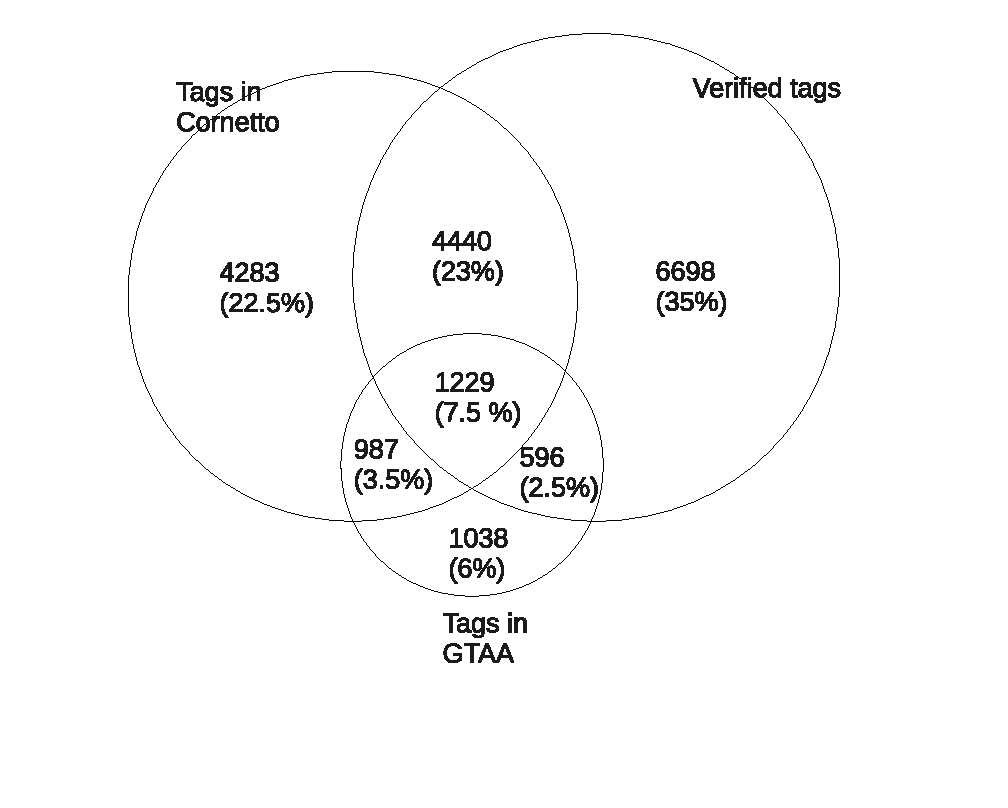
\includegraphics[width=\columnwidth, trim=0 50 0 0, clip=true]{kcap:venn-diagram.eps} 
\caption{Overlap among verified Waisda? tags,  tags in Cornetto, and tags in GTAA. %All numbers are also given as percent (fraction) of the total number of unique tags, 46,792.
}
\label{venndiagram}
\end{figure}

From the total number of tags in total 41\% are either verified or found in
one of the vocabularies. Figure \ref{venndiagram} provides a detailed view of
these tags, showing the overlap between the different sets. We observe that
35\% of the verified tags are not found in either GTAA or Cornetto. Further
investigation revealed that some of these tags do correspond to terms from the
vocabularies, but were not found by the matching algorithm. We also observe
that 32\% (the sum of 22.5\%, 3.5\% and 6\%) of the tags are found in the
vocabularies, but are not verified.

The majority of the tags, approximately 59\%, are neither found in Cornetto
and GTAA nor they are verified. Further analyses revealed that almost half of
these tags are comprised of more that one word. While this could to some
extent explain why they were not found in Cornetto and GTAA (these
vocabularies predominately have single words) and they were not verified
(likelihood of reaching a tag agreement among players decreases as the length
of the tags increases) we still do not know if they are, in fact, meaningful.
To get an answer to this question, we perform additional analysis using Google
as semantic filter. For each tag we carried out a  phrase search (tag was enclosed in quotes, ``")  and observed the number of hits (pages) that were returned. A tag is deemed as meaningful
only if the number of hits returned is positive.

For approximately 84\% of the tags, that were not found verified or not found
in a vocabulary, Google returned positive number of hits. We sampled 200 tags
from the group with no hits (\textit{zero-sample}) and 200 tags with the group
with positive number of hits (\textit{pos-sample}) for further analysis. We
discovered that the tags in the zero-sample could be divided in three groups:
garbled text with no meaning whatsoever, seriously mistyped words (bordering
to garbled text), and entire sentences or excerpts from sentences mostly
grammatically incorrect. The pos-sample, on the other hand, contained
morphological variations of proper words, proper words combined with
characters that are not letters, slang, names, idioms and phrases, and other
common collocations.

In conclusion, the difference between the overlap with GTAA and Cornetto
indicates that the user tags complement the vocabulary used by professional
cataloguers. The tags that are found in GTAA are predominantly subject terms,
but also include locations and names. We also found evidence that user
agreement filters out sloppy tags, as the verified tags are more often valid
Dutch words than the non-verified ones. However, a large part of the
non-verified tags could still be potentially useful, as some of them can be
found in GTAA or Cornetto. Moreover, the majority of non-verified tags were
`deemed' meaningful by Google.


\subsection{Tags in subtitles}
\label{tags-in-transcripts}

\begin{table}[tb]
\centering
\begin{footnotesize}
\begin{tabular*}{\columnwidth}{@{\extracolsep{\fill}}lrr}
\toprule
 \textbf{Episode} \T & \textbf{Tags} &\textbf{Verified tags}\\
 \B & \textbf{in subtitles} & \textbf{in subtitles}\\
\midrule
Farmer seeks wife 1 \T \B & 8,645 (33\%)& 2,546 (43\%)\\
Farmer seeks wife 2 \B &8,004 (35\%)&  2,967 (48\%)\\
Traceless \B & 182 (18\%)& 64 (23\%)\\
Reporter \B & 91 (23\%) &  16 (22\%)\\
The Walk \B & 59 (22\%) & 18 (40\%)\\
\bottomrule
\end{tabular*}
\end{footnotesize}
\caption{Overlap between the Waisda? tags and the video subtitles.}
\label{table:subtitles}
\end{table}

In this experiment we investigate the fraction of \emph{Waisda?} tags that refers to
the audio portion of the video content. To this end, we compare the tags
associated with the five videos described in section \ref{videos} against the
respective video subtitles for hearing impaired persons (see section
\ref{subtitles}). 

Prior to running the analysis, all dialog text from the subtitles was broken
up into words and punctuation through a process known as
\textit{tokenization}. Afterwards, to account for morphological variants, all
words were reduced to their canonical forms through a linguistic procedure
called stemming. Subsequently, the stem of each tag associated with the
aforementioned videos was compared against all words in the subtitles in the
appropriate video that appear at most 10 seconds before the tag was entered.
The time interval of 10 seconds was chosen as a reasonable amount of time
needed by an average player to type in a tag. An identical time interval was
used by the designers of \emph{Waisda?} as the time frame for matching tags added by
different players.

The results of the analysis are summarized in table \ref{table:subtitles}. On
average 26\% of all tags also occur in the subtitles. This number is slightly
higher when it comes to verified tags, on average 35\% of all verified tags
are found in the subtitles. We explain the large overlap by the fact that the
audio stream of the video provides an easy way for the players to score
points. This practice may, however, impair the richness of the user tags. In
addition, when the subtitles of a video are available for retrieval, the user
tags provide less added value.

\subsection{Tag classification}

In this experiment we performed a manual qualitative analysis on the tags of
the five videos described in section \ref{videos}. We only consider the
verified tags of the videos. Due to the prohibitively large number of tags,
for the episodes of \emph{Farmer seeks Wife} we only consider the tags of two
fragments. We excluded 182 tags from the sample since they were words with no
descriptive power, such as particles and prepositions. In total the tag sample
consisted of 1354 tags.

The tags were collectively analyzed by the authors. Each tag was considered in
the light of the video fragment it describes. First, the tags were classified
according to the different levels of abstraction: non-visual, perceptual and
conceptual. We found no tags at non-visual level, and there were only 11 tags
at perceptual level, all referring to colors. The rest of the tags (1,343)
were all conceptual. The vast majority of these conceptual tags, precisely
1,313, were describing objects, whereas only 30 were about scenes. We continue
our investigation by focusing on the conceptual object tags.

In classifying the conceptual object tags we followed the guidelines compiled
by Hollink et. al \cite{laurapaper} --- figure \ref{class_exmpl} shows an
example of a classification of tags for one video fragment. We consider a tag
to be specific if it possesses the property of uniqueness, for example the
name of a person (Anna). A tag is abstract if its level of subjectivity allows
for differences in opinion, for example, ``kind lady'' or ``idyllic
countryside''. We deem a tag to be general when only everyday worldly
knowledge is required to apply it in the context of the video, for example,
``woman'' or ``present''. To determine the facet a tag belongs to, we used the
following guidelines. A tag is in the \textit{who} facet if it refers to the
\textit{subject} (person, object, etc) of the video fragment. A tag belongs to
to the \textit{where} facet if it refers to a location, and to the
\textit{when} facet if it refers to time. A tag is associated with the
\textit{what} facet if it refers to an object or event in the video.

\begin{figure}[tb]
\centering
\subfigure[Keyframe extracted from Farmer seeks Wife episode's shot in which Yvon (the young lady) gives Amsterdam sausage as present to Anna (the elderly lady).]{
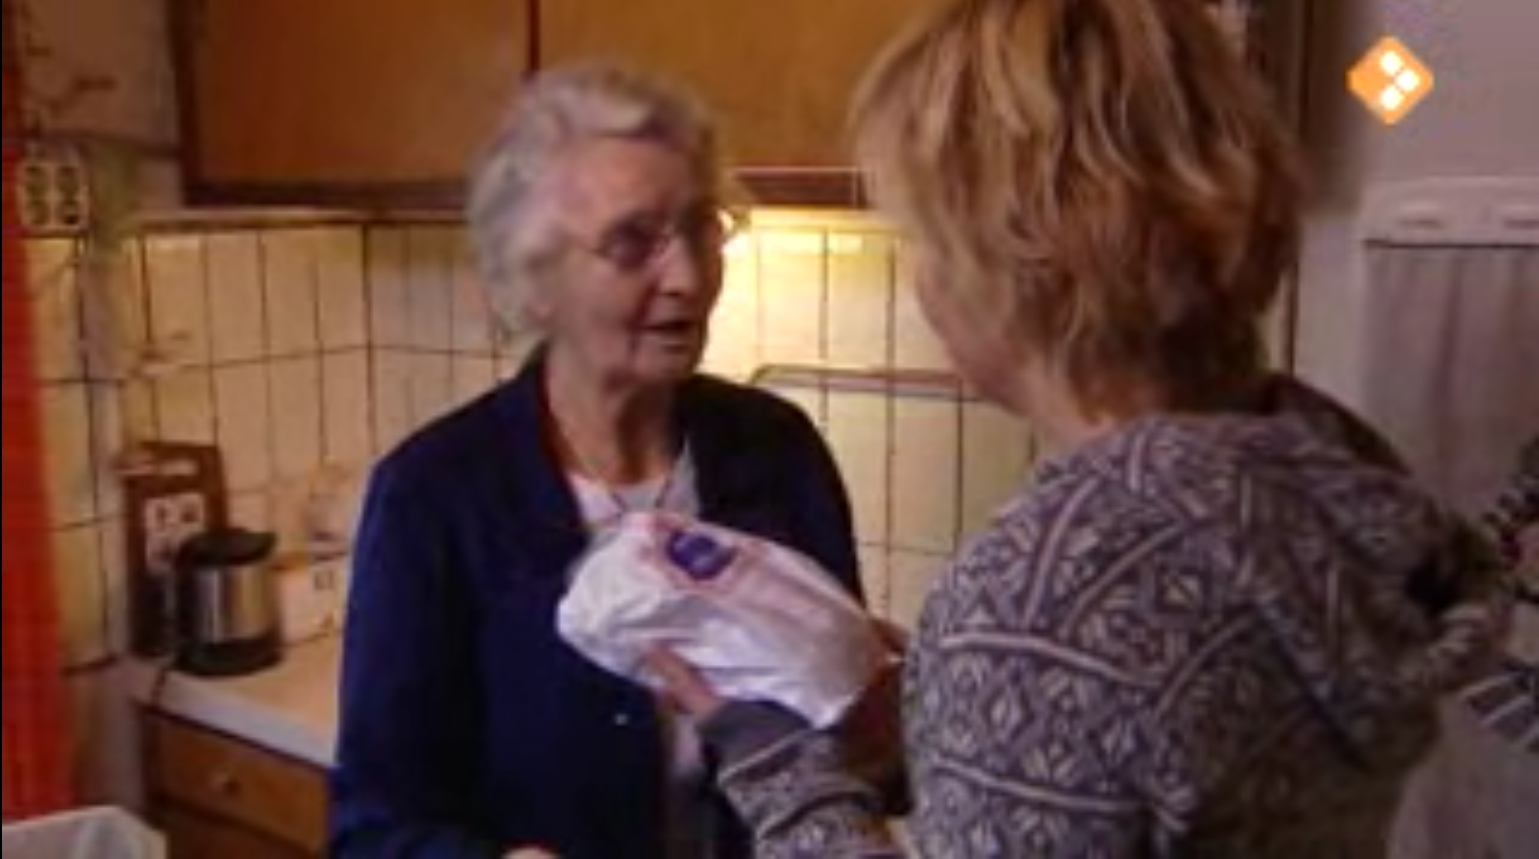
\includegraphics[scale=0.12]{kcap:bzv_screenshot} 
}
\subfigure[Example of how tags (descriptions) of the keyframe above can be classified in terms of the Panofsky-Shatford model.]{
\begin{footnotesize}
\begin{tabular*}{\columnwidth}{@{\extracolsep{\fill}}llll}
\toprule
& \textbf{Abstract} \T \B & \textbf{General} & \textbf{Specific}\\
\midrule
\textbf{Who} \T  & kind & woman &  Anna\\
             \B & lady &  &   \\
\textbf{What} & typical & present & Amsterdam\\
           \B & present &     &    sausage \\
\textbf{Where} &idyllic & kitchen& the Netherlands\\
            \B &countryside & & \\
\textbf{When} & elimination& morning &May 10th\\
	      \B & day & & 2008\\
\bottomrule	      
\end{tabular*}
\end{footnotesize}
}
\caption{Classification of user tags.}
\label{class_exmpl}
\end{figure}

\begin{table}
\begin{footnotesize}
\begin{tabular*}{\columnwidth}{@{\extracolsep{\fill}}lrrrr}
\toprule
\T \B & \textbf{Abstract} & \textbf{General} & \textbf{Specific}  \\
\midrule
\textbf{Who} \T \B & 10 & 166 &  177  & 31\%\\
\textbf{What} \B & 73 & 563 & 12 & 57\% \\
\textbf{Where} \B & 0 & 68 & 8& 7\%\\
\textbf{When} \B & 4 & 31 & 6 & 5\% \\
 \T & 7\% & 74\% & 9\% & \\
\bottomrule
\end{tabular*}
\end{footnotesize}
\label{object_tags}
\caption{Distribution of the object-level tags across the categories of the Panofsky-Shatford model.}
\end{table}


Table \ref{object_tags} shows the distribution of the object-level tags across
the categories of the Panofsky-Shatford model. Looking at the total number of
tags at the different abstraction levels, we observe that the majority of the
tags are general (74\%), while only 7\% are at the abstract level and 9\% at
the specific level. On the other hand, looking at the total number of tags in
the facets, we observe that the majority of the tags belong to the What facet
(57\%). Furthermore, a considerable number of tags are in the Who facet and
only a small number of tags belong to the Where and When facets. Looking at
the relations between the abstraction levels and the facets we observe that
almost all tags in the What facet are general, sometimes abstract, but rarely
specific. The descriptions in the Who facet are, however, at both the general
and the specific level, but rarely abstract. Most of the tags in the Where
facet are generic, and little are specific place or country names. Finally, we
encountered 195 tags that we could not classify in any of the facets. Most of
the time, these tags were modifiers --- typically adjectives and adverbs ---
that describe how an action was performed, for example nice, better etc.

Our results show similarities with classification of image annotations by
Hollink et al.~\cite{laurapaper}. They also found that a large majority of the
descriptions are at the conceptual level. She, however, found a larger number
of scenes (30\%) at the conceptual level. A possible explanation for this
difference could be the fast pace of the game, which makes the player focus on
the directly perceivable objects instead of the overall scene. The evaluation
of the tags by a professional cataloguer also suggested that the users focus
on what can be directly seen or heard. Hollink et. al also found the majority of the descriptions to be at the general level (74\%).

\section{Discussion and future work}
\label{sec:discussion}

In this section we summarize the main observations from our experiments and
discuss to what extent the tags collected with \emph{Waisda?} fulfill the aims
of the Netherlands Institute for Sound and Vision. In addition, we discuss how
the results of our study can improve future versions of the game.

From the comparison of the tags with the terms from the GTAA thesaurus of the
institute and the linguistic database of Dutch, Cornetto, we made several
observations. We can confirm that the aim of the institute to collect metadata
in a user vocabulary can be achieved with the \emph{Waisda?} video labeling game.
Comparable to the results that were found in the Steve.museum tagging project
we found small overlap with the terms in the vocabulary used by professional
cataloguers. In addition, almost half of the verified tags are valid Dutch
words, as they were found in Cornetto. 

The number of verified tags found in Cornetto is much higher than the
number of tags that are not verified. This provides evidence
for the assumption of video labeling games that user agreement on tags can be
used to filter out non-well-formed. We also observed that a large part of
the tags that are not verified could still be potentially useful. A large part
of the non-verified tags could also be found in the vocabularies. In addition,
we deemed most tags meaningful as they returned results from Google.

The manual classification of the tags provides details about the type of tags
that were collected in \emph{Waisda?} and how they relate to the video
content. Users predominately describe \emph{what} appears in the video using
generic tags. Although the tags also provide some coverage of the subject, the
\emph{who}, and the location, the \emph{when} in the video fragments. While
the persons occurring as the subject are described both in generic and
specific tags, there are very few tags describing specific locations.

Together with The Netherlands Institute for Sound and Vision we are preparing
a second pilot project with \emph{Waisda?}. The results of this study show
several limitations of the current metadata, that we aim to address in this
pilot. One limitation is the low number of specific type of tags in the
\emph{who} and \emph{where} facets. We are exploring how users can be
motivated to provide such tags. We showed that by matching the tags to
controlled vocabularies we can derive the type of the tags. We are exploring
if this can be used within the game to detect what type of tags are entered,
and for example provide more points when the user enters a location name. For
this purpose the recall of the current algorithm to match tags and terms
should be improved.

Another characteristic of the current \emph{Waisda?} tags is that many are
also found in the subtitles. In case these subtitles are also available for
retrieval this can be considered a limitation of the tags, as it reduces the
added value. Computing the overlap between the tags and the subtitles during
the game can be used to detect such tags, and for example be used to motivate
users to provide different tags.

An assumption of labeling games is that only the verified tags are associated
to the content as metadata. Our study shows that this approach would exclude
many potentially useful tags. A solution could be to include tags that can be
matched with a term from a controlled vocabulary. Another solution could be to
compare the syntactically different tags based on their semantic similarity.
We are currently exploring the consequences of these methods.

Finally, in future work we will experiment with the usefulness of the tags in
search tasks. From the current results we learned that tags describe what
users directly see or hear in the video. They do not provide a topical description
of a fragment. We expect that the current tags are, therefore, suited to find
objects within a specific video, but are as of yet less useful to find
specific fragments. In future work we will explore methods to also collect
topical descriptions of video scenes, by extending the game and/or with
post-processing of the tags after the game.


\chapter{Game Tags for Visual Video Seach}\label{chap:ecir}

\begin{quotation}
\noindent
In this chapter we start investigating the usefulness of the game tags for search. Throughout this thesis we will address two prominent search scenarios that arise in practice. The first scenario is retrieving video fragments that feature \textit{visual appearances} of objects. In fact, this is very much like the instance search task from TRECVID\footnote{\url{http://trecvid.nist.gov/}} with the difference that query is formulated in text and not by visual example as in TRECVID. The second scenario we consider is topical search i.e. retrieval of video fragments that are about a given topic. In this chapter we study how effective are the game tags in the addressing the first scenario. The methodology that we use is \textit{quantitative system evaluation} \cite{vorhees}. In order to evaluate effectiveness of information retrieval, this methodology requires collection of ``documents'' (in our case video fragments tagged by users via \textit{Waisda?}), set of queries which we derived from real-life query logs, and relevance judgments  indicating which ``documents'' in the collection should be returned for each query. The query set that is created in this chapter is reused in the subsequent Chapter \ref{chap:topicir-filter}, where we address the second scenario.

This chapter was published as ``An Evaluation of Labelling-Game Data for Video Retrieval" in the proceedings of the European Conference of Information Retrieval 2013 \cite{ecir}. It was co-authored with Michiel Hildebrand, Jacco van Ossenbruggen, Lora Aroyo, and Guus Schreiber.
\end{quotation}

\section{Introduction}\label{sec:intro}

Games with a purpose are a way to make humans solve tasks in an entertaining setting. Video tagging games ---a type or GWAPs---	
% is one of the tasks that is being outsourced to internet users. 
%Harnessing users' efforts to amass video annotations 
could become an attractive alternative (or enhancement) to professional annotators in terms of both price and scale. While game tags are virtually for free and plentiful, professional annotations are costly and scarce.
% Consequently, increasing number of video collection owners are deploying GWAPs to collect game tags for their video material. For example,
The Institute for Sound and Vision (S\&V)\footnote{S\&V, \url{http://www.beeldengeluid.nl/}, is the Netherlands national archive.} launched \textit{Waisda?}\footnote{At the time of writing, \textit{Waisda?} is an ongoing project for three years and the game has seen its second release, \url{http://woordentikkertje.manbijthond.nl/}.}, a multi-player video labelling game where players describe streaming video by entering tags and score points based on temporal tag agreement.  The underlying assumption is that tags are faithful descriptions of the videos when entered independently by at least two players within a given time-frame.  From here on we shall refer to such mutually agreed upon tags as \textit{verified} tags.

The archive expects that tags collected with \textit{Waisda?} will improve video search. In this study, we put this hypothesis to the test.
Knowing that other types of video metadata will also be present, our first research question is:
\begin{itemize}
\item[RQ1] Can game tags, on their own or in combination with other types of metatada, improve video search?
\end{itemize}
To test the assumption that agreement is a good filter,  our second research question is:
\begin{itemize}
\item[RQ2] Does limiting only to verified game tags gives better video search performance than considering all game tags?
\end{itemize}
%\textit{RQ3: Which types of video search queries benefit from exploiting game tags?}\\
When GWAPs are used to tag large video collections generally care must be taken to ensure `fair' distribution of game-time across the collection items. In this sense it is instructive for collection administrators and scheduling algorithms designers to know if search performance deteriorates or stagnates after certain point, or if more tags always give better search performance. Therefore, our last research question deals with search performance change over time:
\begin{itemize}
\item[RQ3] How does the game tag search performance change when tags are added?
\end{itemize}

The rest of the paper is structured as follows.  After discussing related work, Sect. \ref{sec:approach} presents our approach. 
Section \ref{sec:materials} describes the datasets and resources that are used in our study. 
%Section \ref{sec:eval-dataset} outlines our evaluation dataset. 
Section \ref{sec:experimental-setup} introduces the experimental setup. Finally, Sect. \ref{sec:results} and \ref{sec:conclusions} present the results and conclusions of this study, respectively.

\section{Related Work}\label{sec:related-work}
\paragraph{User annotations for video.}Video annotation is a tedious and time-consuming activity. Not surprisingly, various initiatives exist that aim at collecting video annotations through crowdsourcing. In particular, \textit{LabelMe video} is an online video annotation system that allows users to identify objects and annotate visual features such as motion and shapes \cite{labelme}. However, this frame-by-frame conceptually low-level annotation remains a tedious task. The willingness of people to participate without compensation is limited at best. To alleviate this, \cite{turk1,turk2} employ the crowdsourcing MTurk platform to recruit annotators which are paid for the task. An alternative way to motivate people is to gamify the annotation experience through GWAPs. GWAPs are computer games, in which people, as a side effect of playing, perform tasks computers are unable to perform. The main example of a GWAP is Luis von Ahn's ESP image labeling game \cite{CHI2004:vonAhn}. Evaluation shows that these labels can be used to retrieve images with high precision and are almost all considered as good descriptions in a manual assessment. The idea to annotate through GWAP has been applied to video in, for example, the Yahoo! video tag game \cite{WWW08_vanZwol_etal}, VideoTag\footnote{\url{http://www.videotag.co.uk/}} , PopVideo\footnote{\url{http://www.gwap.com/gwap/gamesPreview/popvideo/}} and \textit{Waisda?}. With some slight differences, in each of these games players describe streaming video by assigning free-text tags. Thus, we deem \textit{Waisda?} as a typical representative of video GWAPs. 
%What distinguishes \textit{Waisda?} from the other video labelling games is the fact that it was deployed by S\&V with the intention of collecting metadata for improving access to their collection. In this work we study to what extend this is achieved.
\paragraph{Relevance judgements and search.}Designing ground truth in the form of document relevance w.r.t. a given topic has been playing a central role ever since Cranfield experiments gained prominence\cite{vorhees}. The leading actor in IR benchmarking is TREC\footnote{\url{http://trec.nist.gov/}} which employs substantial manpower in creating the ground truth. For organizations lacking the manpower, crowdsourcing is an alternative; \cite{rjturk1,rjturk2} showed that this task can be reliably fulfilled by crowd workers. Alternatively, Eickhoff et al. gamified the task resulting in increased reliability and reduced cost \cite{rjgame}. In this study we also rely on the crowd; the relevance assessment is outsourced to targeted fan groups.\\
Search based on user-generated metadata, in particular folksonomies, has been studied before. Morrison compared the search performance of folksonomies from social bookmarking web sites against search engines and subject directories \cite{morison}, showing that search engines had the highest precision and recall rates. Folksonomies, however, performed surprisingly well. Geisler and Burns state that YouTube tags provide added value for search, because 66\% of them do not appear in  other metadata \cite{youtube}. Hildebrand et al. proposed and investigated a semi-automatic process of assigning explicit meaning to game tags for video by linking them to concepts from the Linked Open Data cloud \cite{michiel}. To the best of our knowledge, no work has been done to evaluate the performance of GWAP data for video search. Our study aims to fill this void.

\section{Approach}\label{sec:approach}
In order to assess the added value of game tags for video search we use a quantitative system evaluation methodology \cite{vorhees}, for which we need a document collection (in our setting video fragments tagged by users in \textit{Waisda?}), a set of representative queries, and relevance judgements.
% System evaluation requires collection of ``documents" (in our case video fragments), set of queries, and relevance judgements indicating which ``documents" in the collection should be returned for each query. 
%For this study we create our own evaluation dataset. Alternatively, we could have used one provided by the various video retrieval evaluation initiatives like TRECVID\footnote{\url{http://trecvid.nist.gov/}}. However, \textit{Waisda?}-like games have not been run yet on these datasets and setting up such a game and attracting sufficient number of users could turn out to be a challenge.
We created this evaluation dataset as follows: (i) select a collection of video fragments tagged by players in \textit{Waisda?}, (ii) select a set of user queries from real-life query logs, and (iii) create relevance judgements. All these steps are described in more detail in Sect. \ref{sec:fragment-collection}.
The dataset is then used in two experiments. In the first, we compare performance of search based on different types of metadata. On high-level the work-flow for the experiment is as follows. We create a number of systems (search engines), run them against the evaluation dataset and compute retrieval performance metrics to assess the search effectiveness of the systems. The structure of all systems is the same: each system uses the same state-of-the-art probabilistic ranking function BM25 \cite{bm25}, but indexes pairwise different combinations of metadata types. Thus, the only variations among the systems within an experiment is the input that they exploit for search. In our experiments we built the systems using the Xapian open source search engine library \footnote{\url{http://xapian.org/}}. We did not vary the parameters for the BM25 function and used the defaults provided by Xapian\footnote{The default parameters for the BM25 algorithm are outlined at \url{http://xapian.org/docs/bm25.html}}. The combinations of metadata types that are indexed by the various systems are strategically chosen so that the resulting performance metrics from the benchmarks will provide answers to the research questions. For example, to determine whether we are better off using all tags opposed to only using verified tags ---remember this is the second research question--- for search, in the first experiment we have a system that indexes \textit{all} game tags and a system that indexes \textit{only the verified} game tags. Since the only difference between these two systems is the metadata they use as input for search, any difference between the search performances will stem solely from the metadata. In other words, by comparing the performance metrics of the two systems we can deduce whether using all tags for search is better than using only the matched ones. To get a better idea of what goes wrong when searching using game tags, we also carry out a follow up analysis of a sample of the results deemed as false positives.
In the second experiment, we study the search performance of game tags over time. To this end, we again create a number of systems, but this time each system indexes a weekly snapshots of all tags. Comparing the performances of the systems that index consecutive weekly snapshots reveals how the tag search performance varies over time.

% The first experiment, described in Section \ref{sec:experiment1-setup}, addresses the first two research questions and the second experiment, presented in Section \ref{sec:experiment2-setup}, addresses the third research question. In both experiments, we create a number of systems (search engines), run them against our evaluation dataset, and compute retrieval performance metrics to assess their performance. All systems use the same state-of-the-art probabilistic ranking function BM25 \cite{bm25} and the only variation among them is the metadata that they index. This way differences in performance can be attributed exclusively to the metadata. Besides the game tags, we exploit the following types of metadata: (i) the existing collection metadata in a form of tags and textual descriptions, and (ii) subtitles (closed captions) associated with the videos. Detailed description of the different metadata types is provided in Section \ref{sec:video-metadata}.

\section{Datasets and Resources}\label{sec:materials}
In this section we describe the datasets and resources that are used in the study.
\subsection{The MBH Video and Metadata Collection}\label{sec:video-metadata-collection}
At the time of writing, \textit{Waisda?} is used to % is in its second release. In this release the collection of fragments that are tagged by players originates from 
tag fragments from the popular Dutch TV program `Man Bijt Hond' (MBH) produced by the Dutch broadcaster NCRV.  MBH is a humoristic TV show that focuses on trivial, everyday news and ordinary and unknown people.  Every episode consists of 7-8 unrelated, self-contained fragments where each fragment topically comes under a recurring heading\footnote{The complete list of the recurring headings (categories) can be found at \url{http://www.manbijthond.nl/rubrieken}. Note that at the time of writing the webpage is in Dutch only.}. Players in \textit{Waisda?} tag these fragments.  The entire collection to which we have access has 11,109 fragments from episodes aired in the last 11 years.

%\begin{table}[tb]
%\centering
%\begin{footnotesize}
%\caption{Descriptive statistics for various video metadata types. Note that \# stands for number. The statistics for the game tags are computed on the subset of 2,192 fragments for which there is at least one user tag and the statistics for the NCRV are computed on the entire collection of 11,109 fragments.}
%\begin{tabular*}{\columnwidth}{@{\extracolsep{\fill}}l|rrr}
%\toprule
%& \textbf{All tags} & \textbf{Verified}&\textbf{NCRV tags} \\  
%\midrule
%\textbf{\# of tags}\B \T &436,456  & 243,352&125,137\\
%\textbf{\# of unique tags}\B &47,455  &12,861  & 25,760\\
%\textbf{avg. \# of tags per video}\B& 199 &111& 11.4\\
%\textbf{min. of \# of tags per video}\B&1 &2&1\\
%\textbf{max. of \# of tags per video}\B&3,700 &3147&105\\
%\textbf{median of \# of tags per video}\B&65 &76&11\\
%\bottomrule
%\end{tabular*}
%\end{footnotesize}
%\label{table:tags-stats}
%\end{table}

% \subsection{Video metadata}\label{sec:video-metadata}

In addition to the video fragments, we have access to four types of descriptive metadata that are used as input for search:
\paragraph{\textbf{Waisda? tags.}} We consider the collection of all game tags acquired with \textit{Waisda?} during the first five months, starting from October, 2011. In this period 436,456 different tag entries were assigned to 2,192 video fragments by roughly 24,000 players. The number of unique game tags exceeds 47,000. Each tag entry is associated with the point in time --- relative to the beginning of the fragment --- when the tag was entered. Additionally, each tag entry is marked as `verified' or not based on the tag agreement in its temporal neighbourhood.
%In particular, a tag is verified if it is entered by at least two distinct players in a time interval of 10 seconds.
As the game is advertised only in Dutch media and the material being tagged is exclusively in Dutch, the language of almost all tags is Dutch. The average number of tags per video is 199. Approximately 55\% of all game tags ($\approx$ 243,000) are `verified' and the number of unique verified tags is 12,861. The average number of verified tags per video is 111.
\paragraph{\textbf{NCRV tags.}} NCRV, the broadcaster, maintains an in-house collection of tags % that describe their video material. The purpose of these tags is 
to facilitate web access to MBH fragments via search and browsing. In contrast with \textit{Waisda?} tags, NCRV tags are not time-based, meaning they are not linked to a particular time-point in the video, and generally cover only the prevalent topics. The average number of NCRV tags per video is 11. Thus they are usually much scarcer than the game tags.
\paragraph{\textbf{NCRV catalogue data}.} Along with the curated NCRV tags, each MBH fragment has a short textual description, usually one paragraph, and a title. We consider the collection of all titles and textual descriptions (i.e. catalogue data) as another metadata type that will be used in the study.
\paragraph{\textbf{Captions}.} % Yet another metadata type we make use of is the subtitle files associated with the video fragments. 
Closed captions are textual versions of the dialogue in films and television programs for the hearing impaired, usually displayed at the bottom of the screen. Each dialogue excerpt is accompanied with time-points --- relative to the beginning of the video --- when the dialogue excerpt appears on and disappears from the screen. We use captions  obtained from S\&V\ that cover most of the MBH episodes aired in 2010 and 2011 which amounts to a total of 897 fragments. 

\begin{figure}[t]
\centering
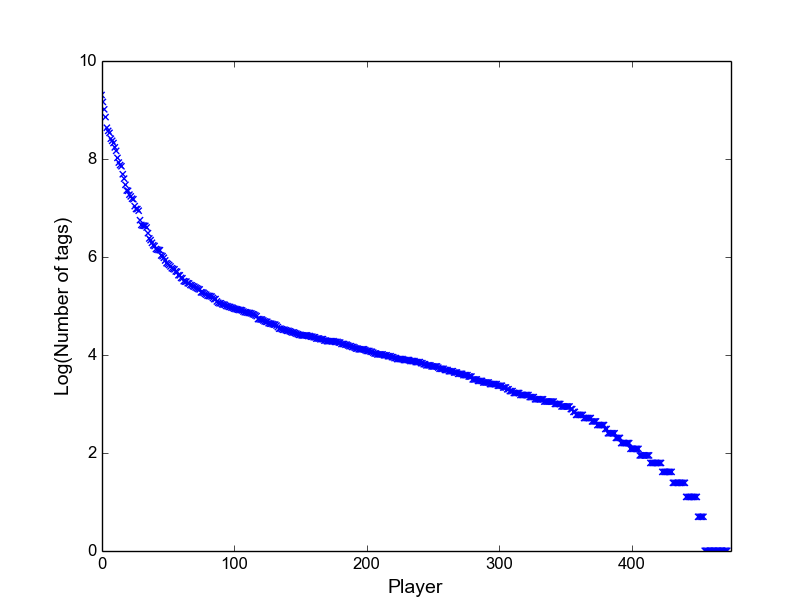
\includegraphics[scale=.4]{ecirnumtagsperplayer} 
\caption{Number of tags contributed by each of the players in the selected sample of fragments. The horizontal axis represents the players ordered decreasingly on the number of tags they entered. The vertical axis displays the logarithm to base 2 of the number of tags entered by the associated player.}
\label{numtagsperplayer}
\end{figure}

\subsection{Evaluation Dataset}\label{sec:eval-dataset}
In this section we describe the creation of the three separate components of our evaluation dataset: set of video fragments, set of queries, and relevance judgements.
\paragraph{\textbf{Video fragment subset.}}
\label{sec:fragment-collection}
The set of fragments for our experiment is selected from the MBH fragments tagged in \textit{Waisda?}. Not all metadata types described above are available for every single fragment. To do a fair comparison of the search performance of various metadata types, we use only a subset. The filtering criterion is as follows: we include only the fragments that have at least one \textit{Waisda?} tag and NCRV tag ascribed to them, and for which captions files are available. This results in a collection of 197 fragments. The accumulative duration of our test collection is almost 11 hours of video material, with an average fragment length of approximately 3.3 minutes and a median of 3.6 minutes. The duration of the shortest and the longest fragment in our collection is 0.5 and 8.6 minutes, respectively. The total number of game tags, verified game tags, and NCRV tags ascribed to the the videos of these collection is 107,531, 80,805, and 2,066, respectively. Thus, the average number of game tags, verified game tags, and NCRV tags per fragment is 545, 410, and 10 respectively. Figure \ref{numtagsperplayer} displays the number of tags contributed by each of the players in the selected sample of fragments. The number of players that entered at least one tag for one of the fragments in the sample is 473. As can be seen from the figure there is a small core of power taggers which contributed significant portion of the tags. In fact, each of the top ten players has entered more than 500 tags. The median number of tags entered by a player for the sample of fragments is 28.
%\textsc{\begin{figure}
%\centering
%\includegraphics[scale=.325]{fragmentdurationhist.jpeg}
%\caption{Distribution of the duration (in minutes) of the fragments in our collection.}
%\label{fig:fragment-duration-histogram}
%\end{figure}}

\paragraph{\textbf{Query set.}}\label{ecir-sec:query-set}
To measure the information retrieval performance we use real-life user queries. NCRV provided us with one month of query logs from the MBH web site. The logs contain 15,219 queries posed by the internet users to the site's search engine asking for video fragments. Figure \ref{fig:query-frequency} shows the query frequency distribution. As seen, the query frequency follows a power law; aside from few frequent ones most of the queries appear infrequently. In fact, only 6\% of the queries appear at least 5 times (points under or on the lower horizontal dashed line in Figure \ref{fig:query-frequency}).

\begin{figure}[tb]
\centering
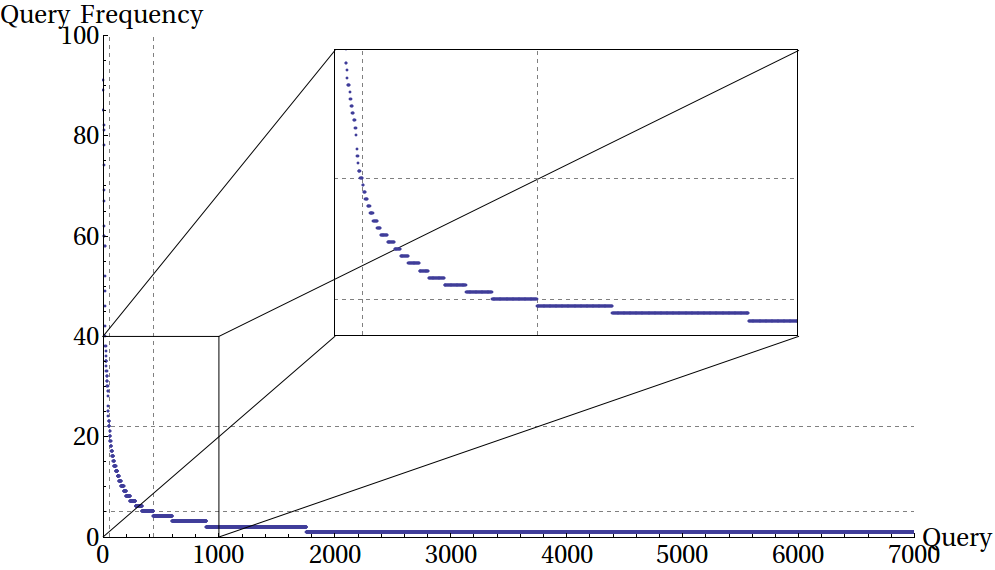
\includegraphics[scale=.3]{ecir:query-freq}
\caption{Query frequency distribution. Horizontal dashed lines represent the ``appeared 5 times" and ``appeared 22 times" thresholds when observing from bottom to top. Vertical lines divide the area under the curve in three equal parts.}
\label{fig:query-frequency}
\end{figure}

% \subsubsection{Query selection procedure} 
Out of the complete set of 15,219 user queries we select, in two steps, a subset of 50 queries to include in the study. 
First, we partition the query set into three classes: a high, mid and low frequency class. The borders of the classes are chosen so that the area under the curve in Figure \ref{fig:query-frequency} for each class is one third of the area. Queries appearing more then 22 times form the high-frequency class, between 5 and 22 form the middle-frequency class, and queries appearing less than 5 times form the low-frequency class.

Second, for each class we perform filtering. Namely, a query is skipped whenever it meets one of the following criteria: (i) it equals the title of one of the MBH recurring headings or it contains one of the words `man', `bijt', and `hond' from the series title. (ii)  it is not found in at least two of the metadata types described in Sect. \ref{sec:video-metadata-collection}. We consider the first criterion in order to exclude the non-informative queries\footnote{Queries that are expected to have a high \textit{inverse document frequency} (IDF)} and we consider the second criterion to avoid creating bias towards any metadata type. After the filtering, we are left with 12, 78, and 49 queries from the high-frequency, middle-frequency, and low-frequency class, respectively.
%\footnote{We use xapian (\url{http://xapian.org/}) IR library to implement basic search engines that index the various metadata types.}.
%We include the last criterion to avoid creating a bias in our query set towards a particular metadata type.\\
%Note that the verified \textit{Waisda?} tags were not considered as a separate metadata type from complete set of \textit{Waisda?} tags.
%In the final phase we sort the queries in each stratum on the sum of the number of videos returned by each metadata type. The count from the verified \textit{Waisda?} tags is excluded as these videos are already accounted for by the complete set of \textit{Waisda?} tags.
The top 12, top 19, and top 19 queries from the high-frequency, middle-frequency, and low-frequency class, respectively, comprise the final query set. All queries in the query set are single-term queries. This is a consequence of our second selection criterion --- the requirement of a query being present in at least two metadata types which reduces the probability of multi-term queries being selected. The second selection criterion was introduced mainly to be fair towards NCRV tags and catalog data. Our analysis of the query logs revealed that generally queries were present either in the \textit{Waisda?} tags or the captions, sometimes both. In contrast, the queries from the query logs were less frequently present in the NCRV metadata. Thus, if we omit this criterion --- and potentially include multi-term queries --- out expectation is that it will not drastically change the outcome for the \textit{Waisda?} tags and the captions. However, the NCRV metadata will likely perform worse.

\paragraph{\textbf{Relevance judgements.}}\label{sec:gold-standard}
In order to collect relevance judgements for the query set and the fragment collection we performed an on-line user experiment. To this end, we deployed a web application which was used by the participants to carry out the evaluation. %At the time of writing, the application is still up and running and it can be accessed at \url{http://tinyurl.com/c6c494v} (Dutch only).
For each participant the workflow proceeds as follows. Whenever a participant accesses the web application she is presented with a welcome page which contains a description of the task she is required to perform. Before starting with the evaluation, the participants need to fill out a questionnaire that aims at assessing their familiarity with \textit{Waisda?}, the MBH TV series and the MBH website. Then the participants proceed to the evaluation page (see Figure \ref{fig:evaluation-page}) which plays a randomly assigned fragment and lists the complete query set. During the evaluation process, the participants watch the fragment and indicate which of the concepts denoted by the queries are shown in it. \textit{We asked users to judge a fragment to be relevant for a query if it depicts the concept denoted by the query}. Each participant is asked to evaluate at least five fragments.
\begin{figure}
\centering
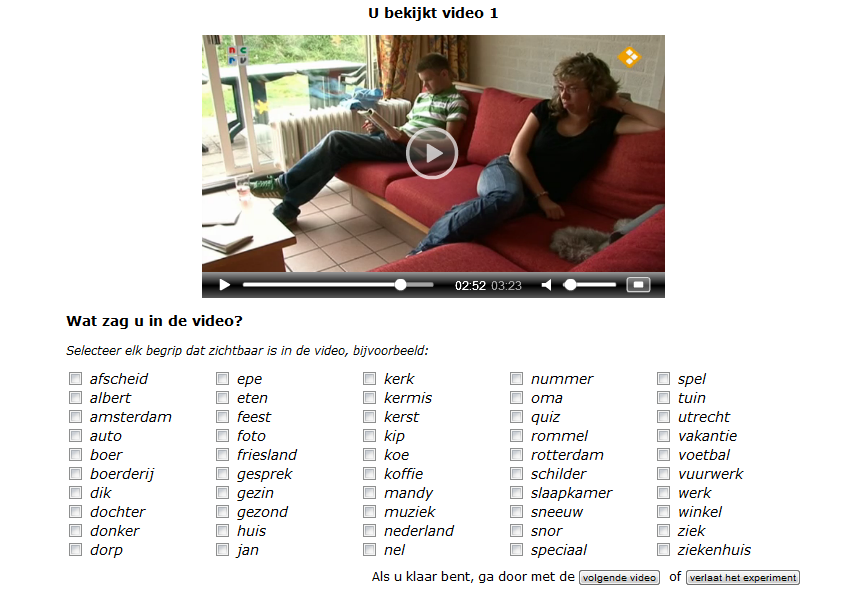
\includegraphics[scale=.5]{ecir:mendyvideo.PNG}
\caption{Screenshot of the evaluation page. At the top, a video player is placed which displays the fragment. The list of queries is rendered at the bottom.}
\label{fig:evaluation-page}
\end{figure}


\subsubsection{Participants}
The participants in the experiment were recruited mainly from the \textit{Waisda?} online community and MBH series fanbase by distributing a call for participation through the major social networking services Facebook\footnote{\url{http://www.facebook.com/}} and Twitter\footnote{\url{https://twitter.com/}}. The posted messages and tweets contained a link to our web application. 107 participants started the experiment, 83 of them evaluated at least one fragment and 25 participants evaluated more than 5 fragments. 
%Figure \ref{fig:number-of-evaluations} shows in more detail the distribution of the number of evaluated videos per participant.
Judging from the questionnaire data, the level of familiarity of participants with MBH series almost uniformly ranges from `never seen it' to `watch it regularly'. Surprisingly, the participants who never visited the MBH website or visited it only few times are the vast majority.  Also for familiarity with \textit{Waisda?}; the participants who never played or played only few times are the overwhelming majority.
%\begin{figure}
%\centering
%\includegraphics[scale=.4]{numberofevaluations.jpeg}
%\caption{Distribution of number of evaluated videos per participant.}
%\label{fig:number-of-evaluations}
%\end{figure}

\subsubsection{Participant's (Dis)agreement}
From the entire collection of 197 video fragments, 134 of them are evaluated by 2 distinct participants. The rest of the fragments, 63 in total, are evaluated by 3 distinct participants. When consolidating the relevance judgements from different participants we use majority voting; the side --- either `relevant' or `not relevant' --- that gets more votes wins. In case of a tie, we take the side of `relevant' i.e. we deem the fragment to be relevant for the query. We justify this decision with the following reasoning. The notion of relevance in our particular case is defined in terms of depiction of the concept denoted by the query in the fragment. Our queries are not abstract concepts and there is very little room for different interpretations among the participants. Thus, we believe if one participant rated  a query `not relevant' and another `relevant' for a given fragment it is most probable that the first participant simply missed it. The consolidated evaluation set is publicly available online at \url{https://goo.gl/AQcpGz}. 
The overlap among the participants in terms of evaluated videos is too small to reliably measure the inter-rater agreement with measures such as Krippendorff's alpha. However, we found that the probability of a rater rating `relevant' is 9.5\% and the probability of disagreement between raters is 10.1\%.

\section{Experiments}\label{sec:experimental-setup}
To answer the research questions formulated in Sect. \ref{sec:intro} we use a quantitative system evaluation. Namely, we implement a number of search engines and run them against the evaluation dataset described in Sect. \ref{sec:gold-standard}. In all experiments we evaluate the performance of the various search engines using the mean average precision (MAP) measure. The number of results returned by the systems is low enough (not more than 30) for the users to be willing to inspect them all. Thus, we deem that it is important that all results are good not just the top ones. This intuition is captured by MAP. To assess if the difference in performance is statistically significant we use the student's paired t-test at 0.01 level of significance as suggested by \cite{stat-sig}.

\subsection{Experiment 1}\label{sec:experiment1-setup}
In this experiment we address the first and the second research question. To this end, we retrieve fragments for the set of queries using 12 search engines. Each of the search engines utilizes the same state-of-the-art probabilistic ranking function BM25 and the only variation among them is the data they index. Consequently, differences in retrieval performance are attributed solely to the data. We implement search engines that index:

\begin{tabular}{lll}
 1. & $SE_{user}$  & all \textit{Waisda?} tags \\
 2. & $SE_{vuser}$& only verified \textit{Waisda?} tags \\
 3. & $SE_{ncrv}$& all NCRV tags \\
 4. & $SE_{catalog}$&  NCRV catalogue data \\
 5. & $SE_{caps}$& all captions\\
 6. & $SE_{caps+user}$&  all captions and all \textit{Waisda?} tags \\
 7. & $SE_{caps+catalog}$& all captions and all catalogue data \\
 8. & $SE_{ncrv+caps}$&  all captions and all NCRV tags \\
 9. & $SE_{ncrv+user}$&  all NCRV tags and all \textit{Waisda?}  tags \\
 10. & $SE_{ncrv+catalog}^{baseline}$& all NCRV tags and catalog data \\
 11. & $SE_{all-user}$&  all metadata  except  \textit{Waisda?} tags \\
 12. & $SE_{all}$&  all metadata types including  \textit{Waisda?}  tags \\
\end{tabular}

\noindent
$SE_{ncrv+catalog}^{baseline}$ is an approximation of the search functionality offered on the web site dedicated to MBH series. We use it as a baseline for comparing the search performance of the other search engines. By comparing the performance of $SE_{user}$ and $SE_{vuser}$ we are able to see if using all tags as opposed to only verified tags is detrimental or beneficial for fragment search (\textit{RQ2}). Furthermore, comparing the performance of $SE_{user}$ and systems 3 through 12 will reveal how well game tags are doing --- on their own and in combination --- compared to other types of metadata (\textit{RQ1}).

%\subsubsection{Experiment 2}
%The goal of this experiment is to answer the third research question. Once again, we retrieve fragments using the $SE_{user}$, $SE_{vuser}$,  $SE_{ncrv}$, $SE_{catalog}$, and $SE_{subs}$ search engines from the previous experiment. However, this time we consider several query subsets, where each subset contains queries classified in specific category of the Panofsky-Shatford model. By comparing the performance of the search engines across difference categories of the Panofsky-Shatford model we will see for which type(s) of queries game tags are best suited.

\subsection{Experiment 2} \label{sec:experiment2-setup}
In this experiment we address the third research question. We retrieve fragments for the set of queries using two collections of search engines. The first collection consists of search engines that index snapshots\footnote{A snapshot contains all game tags up to a given point in time.} of all game tags taken periodically once a week. Identically, the second collection consists of search engines that index snapshots of the verified tags taken at the same time points as the snapshots from the first collection. As with experiment 1, all search engines use the same probabilistic ranking function BM25 and the only variation among them is the data that they index. Examining the performance of search engines within a collection reveals how tag search performance changes over time. By examining the performance of search engines across collections we learn how all tags perform compared to verified tags.

\section{Results}\label{sec:results}
In this section we present the results of our experiments.
\subsection{Experiment 1}
The results for this experiment are summarized in Table \ref{table:results}. As seen, considering only verified tags yields worse search performance than considering all tags. Intuitively, verified tags should yield higher precision but lower recall than all tags. Indeed, the average search precision of verified tags (0.59) across the queries is higher than the average search precision of all tags (0.49). However, search based on all tags yields more relevant results --- the average search recall of all tags (0.42) is higher than the averages search recall of the verified tags (0.28). In fact, for 35 queries the non-verified tags yielded relevant results ---on average 4---not found by verified tags\footnote{More detailed figures can be found the Appendix \ref{appen:prec-recall} at the end of the thesis.}. It seems the \textit{tag verification} criterion is too conservative in a sense that it filters out tags that are in fact useful for search.

Search based on game tags ($SE_{user}$) significantly outperforms search based on other metadata types alone. Indeed, search based on game tags is approximately 69\% more successful than search based on the in-house NCRV tags ($SE_{ncrv}$). We believe this is attributed to the fact that NCRV tags are relatively scarce and cover mainly prevalent topics. In this sense, game tags are complementary to the NCRV tags and the combination of both is mutually beneficial. Indeed, the search engine that indexes both game tags and NCRV tags, $S_{ncrv+user}$, yields a performance increase of 20\% and 90\% over search engines $S_{user}$ and $S_{ncrv}$, respectively.\\
Furthermore, search based on solely on game tags yields better performance from our baseline search engine, $SE_{ncrv+catalog}^{baseline}$. Indeed, the MAP scores of $S_{user}$ and $SE_{ncrv+catalog}^{baseline}$ indicate a performance increase of 46\%.\\
Comparison of the MAP scores of $SE_{user}$ and $SE_{caps}$ indicates that game tags outperform captions by approximately 39\%. This can be explained by the fact that captions only cover the audio portion of the video content, whereas game tags cover both audio and visual. In fact, previous work \cite{kcap} suggested that players tend to describe more things that appear visually in a video. Combination of captions and game tags proves to be beneficial: $SE_{caps+user}$ outperforms $SE_{caps}$ and $S_{user}$ by 64\% and 13\%, respectively.\\
Lastly, the search engine that indexes all available types of metadata, $SE_{all}$, performs best. This is to a large extend due to the contribution of game tags. Indeed, $SE_{all}$ outperforms the search engine that indexes all metadata types except for game tags, $SE_{all-user}$, by 33\%. Obviously, the said difference can only be attributed to the effect of the game tags. Interestingly, search based on game tags alone outperforms by 5\%  $SE_{all-user}$, which is the best performing search engine that does not index game tags.

\begin{table}[tb]
\centering
\begin{footnotesize}
\label{table:results}
\begin{tabular}{l|l|l|l}
\toprule
$SE_{user}$ & $SE_{vuser}$ & $SE_{ncrv}$ & $SE_{catalog}$\\
\hline
$0.219^{\approx \uparrow}$ & $0.143^{\downarrow \approx}$ & $0.138^{\downarrow \downarrow}$ & $0.077^{\downarrow \downarrow}$\\
\hline
\multicolumn{4}{c}{ }\\
\hline
$SE_{caps}$ & $SE_{caps+user}$ & $SE_{caps+catalog}$ & $SE_{ncrv+caps}$\\
\hline
$0.157^{\downarrow \uparrow}$ & $0.247^{\uparrow \uparrow}$ & $0.183^{\downarrow \uparrow}$ & $0.201^{\downarrow \uparrow}$ \\
\hline
\multicolumn{4}{c}{ }\\
\hline
$SE_{ncrv+user}$ & $SE_{ncrv+catalog}^{baseline}$ & $SE_{all-user}$ & $SE_{all}$\\
\hline
$0.263^{\uparrow \uparrow}$ & $0.150^{\downarrow \uparrow}$ & $0.208^{\downarrow \uparrow}$ & $0.276^{\uparrow \uparrow}$ \\
\bottomrule
\end{tabular}
\caption{Results for experiment 1: MAP scores for the search engines --- MAP score for given search engine is given immediately bellow. $\uparrow$, $\downarrow$, and $\approx$ indicate if a score is significantly better, worse, or statistically indistinguishable from the MAP scores of $SE_{user}$ and $SE_{vuser}$, in that order.}
\end{footnotesize}
\end{table}


%\begin{table}[tb]
%\centering
%\begin{footnotesize}
%\begin{tabular}{cl|r|r|r|r|r}
%\toprule
%  & \multicolumn{5}{c}{\textbf{Query set}}\\
% \cline{3-7}
%& & \textit{All} & \textit{A-What} & \textit{G-What} & \textit{G-Where} & \textit{G-Who}   \\
%\cline{2-7}
%\multirow{1}{*}{\rotatebox{90}{\textbf{Search engine}}}&\multicolumn{1}{|l|}{$SE_{user}$}& $0.219^{\approx \uparrow}$ &  &  &  &  \\ 
%\cline{2-7}
% & \multicolumn{1}{|l|}{$SE_{vuser}$} & $0.143^{\downarrow \approx}$\\
% \cline{2-7}
% & \multicolumn{1}{|l|}{$SE_{ncrv}$} & $0.138^{\downarrow \downarrow}$\\
% \cline{2-7}
% & \multicolumn{1}{|l|}{$SE_{catalog}$}& $0.077^{\downarrow \downarrow}$\\
% \cline{2-7}
% & \multicolumn{1}{|l|}{$SE_{subs}$} & $0.157^{\downarrow \uparrow}$ \\
%  \cline{2-7}
% & \multicolumn{1}{|l|}{$SE_{subs+user}$}&  $0.247^{\uparrow \uparrow}$\\
%  \cline{2-7}
% & \multicolumn{1}{|l|}{$SE_{subs+catalog}$}&  $0.183^{\downarrow \uparrow}$\\
%  \cline{2-7}
% & \multicolumn{1}{|l|}{$SE_{ncrv+subs}$}&  $0.201^{\downarrow \uparrow}$\\
%  \cline{2-7}
% & \multicolumn{1}{|l|}{$SE_{ncrv+user}$}& $0.263^{\uparrow \uparrow}$\\
%  \cline{2-7}
% & \multicolumn{1}{|l|}{$SE_{ncrv+catalog}^{baseline}$}& $0.150^{\downarrow \uparrow}$\\
%  \cline{2-7}
% & \multicolumn{1}{|l|}{$SE_{all-user}$} & $0.208^{\downarrow \uparrow}$\\
%  \cline{2-7}
% & \multicolumn{1}{|l|}{$SE_{all}$} & $0.276^{\uparrow \uparrow}$
%
%\bottomrule
%\end{tabular*}
%\end{footnotesize}
%\caption{Results for experiment 1 and experiment 2: MAP scores for several query sets and 8 search engines. $\uparrow$, $\downarrow$, and $\approx$ indicate if a score is significantly better, worse, or statistically indistinguishable from the MAP scores of $SE_{user}$ and $SE_{vuser}$, in that order.}
%\label{table:results}
%\end{table}

%\subsection{Experiment 2}

\subsubsection{Analysis of False Positives}
One of the conclusions drawn above is that the precision of $SE_{user}$ ---or in other words when considering all game tags --- is relatively low. In order to get a better insight into the reasons that lead to poor precision we manually analysed a sample of the false positives\footnote{A search result is a false positive if it is returned by $SE_{user}$ but was deemed `not relevant' by our evaluators.} among the results obtained from $SE_{user}$ . Note that given the definition of search precision, it is the false positives that are accountable for the drop in the precision score.

In the course of the analysis, we randomly picked fifteen queries from the query set and investigated the false positives retrieved for them --- 192 in total. For each query-fragment pair we watched 10 seconds prior and 10 seconds after the point when the tag that matched the query was entered. The occurrence of the query instance in the fragment is then classified as either `visual', `nonvisual' based on the same criterion used by the evaluators, or \textit{unrelated}. The \textit{unrelated} category consists of tags that are not describing the content of the video and can be accounted as errors by the users. The `visual' class is further subdivided into the following disjoint subclasses which designate how/where the instance denoted by the query is depicted along the spatial and temporal dimensions:
\begin{itemize}
\item \textit{Intro}. The instance is in the opening segment of the fragment which is usually unrelated with the rest of the fragment.
\item \textit{Short-lived in background}. The instance appears for a brief moment, e.g. less than a second, in the background and not in opening segment. An example of this would be a \textit{car} passing by in the background.
\item \textit{Short-lived in foreground}. The instance appears for a brief moment, e.g. less than a second, in the foreground and not in opening segment. An example of this  would be a \textit{person} passing by in front of the camera.
\item \textit{Long-lived}. The instance appears either in the background or in the foreground for a longer period of time.
\end{itemize}
The `nonvisual' class is subdivided into the following disjoint subclasses:
\begin{itemize}
\item \textit{Captions in intro}. The instance appears only in captions in the opening segment.
\item \textit{Captions}. The instance appears only in captions and not in the opening segment.
\item \textit{Screen text}. Screen text referring to the instance.
\end{itemize}
The results of the classification are summarized in Table \ref{tab:exp1-false-pos}. As seen, significant fraction of the false positives were caused from tags associated with the opening segments: 17\% of them refer to visual instances and 12\% are mentioned in the captions in the opening fragment. Moreover, 15\% of the false positives are a result of the tags found only in the captions not in the opening segments. In general, it is context-dependent whether these cases should be considered relevant or not. In this analysis, we deemed visual appearances in opening segments as relevant and references in captions as not relevant due to our interpretation of (visual) relevance. However, in other scenarios the interpretation of relevance may differ. Nevertheless, it is straightforward to detect these cases automatically and include/exclude them as input for search depending on the context.
The \textit{short-lived background/foreground} and \textit{other} cases were most likely missed by the evaluators. Had they been correctly identified the outcome of the comparison given above would have been even more favourable for \textit{Waisda?} tags. 
Furthermore, 20\% of the false positives were visual appearances of long-lived instances i.e. objects appearing on screen for a longer period of time. However, it is interesting to mention that these cases usually involved ambiguity and the context and the hints provided by the current or the previous scenes from the video were required to make the correct interpretation. For example, for the query \textit{boer} (the Dutch word for \textit{farmer}) there were instances where a person while being a farmer, a fact established in the previous scenes, in one particular scene was not in the typical farmer's attire and could not be identified as such using only the information provided on the screen. It is easy to imagine how a tagger having seen the video from the beginning and having this extended context could interpret the person as a farmer. Needless to say, what is the right answer in these cases depends on the particular application context. Finally, 21\% of the false positives were caused by incorrect tags not at all related with the content of the fragments.

\begin{table}[tb]
\centering
\begin{footnotesize}
\begin{tabular*}{\columnwidth}{@{\extracolsep{\fill}}lrr}
\toprule
\multirow{4}{*}{\textbf{Visual}} & \textit{Intro}  \T \B & 33 (17\%) \\
  %\cline{2-3}
 & \textit{Short-lived in background} \T \B & 13 (7\%)\\
 & \textit{Short-lived in foreground} \B &  15 (8\%)\\
 & \textit{Long-lived} \B & 38 (20\%)\\
\hline
\multirow{4}{*}{\textbf{Nonvisual}} & \textit{Captions in intro} \B \T & 23 (12\%)\\
%\cline{2-3}
 & \textit{Captions} \T \B &  28 (15\%)\\
 & \textit{Screen text} \B & 1 (0\%)\\
 \hline
 &&\\
 \textbf{Unrelated} & &  41 (21\%) \\
 &&\\
\bottomrule
\end{tabular*}
\end{footnotesize}
\caption{Experiment 1 false positives classification.}
\label{tab:exp1-false-pos}
\end{table}


\subsection{Experiment 2}\label{ecir:over-time-results}
In this section we present the results from our second experiment which addresses the third research question. Figure \ref{fig:snapshop-map} shows the MAP scores of the search engines indexing the weekly snapshots of all tags and only the verified tags. Figure \ref{fig:snapshot-tcount}, on the other hand, shows how the number of all tags and verified tags increased over time.
Looking at Figure \ref{fig:snapshop-map} we conclude that most of the time the search performance for both the verified tags and all tags is monotonically increasing with the number of tags. In other words, the more tags we amass, the better our effectiveness in searching fragments becomes. Furthermore, looking at the pairwise search performance differences between the search engines that index the weekly snapshots of all tags and verified tags (vertical dashed lines between plots in Figure \ref{fig:snapshop-map}), we conclude that using all tags for search opposed to only verified ones yields consistently better results. In fact, search performance improvements are statistically significant for every single pair.

The performance of search based on all game tags surpasses our baseline, $SE_{ncrv+catalog}^{baseline}$, around the $11^{th}$ week after 42,271 tags have been collected (Figure \ref{fig:snapshot-tcount}). Beyond that point the said difference in performance steadily increases as more tags are collected. With $SE_{all-user}$, which is the best performing search engine that does not index game tags, this happens a bit later. In particular, after the $18^{th}$ week and 91,508 collected tags, $SE_{user}$ starts to outperform $SE_{all-user}$. Thus, there is a point somewhere between the $18^{th}$ and $19^{th}$ week when the collected game tags outperform all search engines that do not index tags.

It is also interesting to note that the precision and recall of search based on all tags are monotonically non-decreasing with the number of tags for each query in our set. The results for search precision and recall can be found in the appendices \ref{appen:precovertime} and \ref{appen:recovertime} at the end of the thesis, respectively.

\begin{figure}
\subfigure[The MAP scores of the game tags over time. Horizontal lines represent MAP scores of $SE_{ncrv+catalog}^{baseline}$ and $SE_{all-user}$]{
	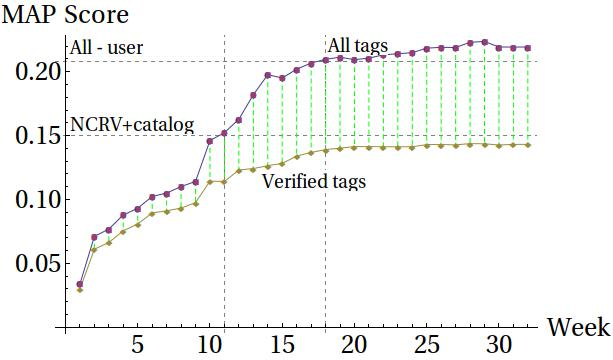
\includegraphics[scale=.28]{ecir:snapshots-map.jpeg}
	\label{fig:snapshop-map}
}
\subfigure[The total number of tags over time]{
	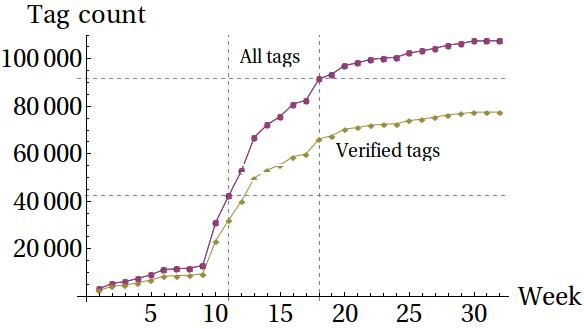
\includegraphics[scale=.3]{ecir:snapshots-tag-count.jpeg}
	\label{fig:snapshot-tcount}
}
\caption{MAP scores and tag count over time.}
\end{figure}

\section{Conclusions and Future Work}\label{sec:conclusions}
In this paper we have studied the added value of game tags for video search. For this reason we have created a publicly available evaluation dataset that consists of real-life user queries, a video fragment collection, and relevance judgements. 

Search based solely on game tags outperforms search based on other types of metadata such as in-house (NCRV) tags or captions. Thus if any of the other metadata types are unavailable or costly to acquire, relying only on sufficient game tags for search could yield equal or even better results. In our dataset, combining game tags with other metadata types is beneficial for search. In fact, the search engine that exploits all available metadata performs best, to large part due to the contribution of the game tags---the observed performance improvement is 33\%. 

Exploiting only verified game tags for search gives poorer performance than search based on all game tags. While search based on verified tags yields higher precision, it also has lower recall compared to all game tags. In fact, for most of the queries non-verified tags provided relevant results that were not found by the verified tags. This proves that considering only verified tags is too conservative filtering criterion resulting in discarding non-verified game tags that are valid video descriptors and thus useful for search. 

Search performance steadily increases as more game tags are collected. This is true for both verified and all tags. Moreover, search based on all tags consistently outperforms search based only on verified tags. When the average number of tags is slightly more than 2 tags per second, the search using all tags outperforms all search engines that are not indexing game tags. Such an estimate could be used as an indicator whether a video has been tagged enough.

In Chapter \ref{chap:ecir} we established that game tags usually describe events and objects within scenes so it is not surprising that they excel at visual search. We also established that there is a difference in the focus and the scope of the game tags compared to the professional annotations; game tags being more fine-grained and professional annotations being more coarse-grained referring to the entire video and describing the prevalent topics. The in-house catalogue tags fit the latter profile: they are scarce and cover the topics of the video. This being said, quite predictably they fall short compared to the game tags when it comes to visual search. The closed-captions, on the other hand, are similar to the game tags in terms of focus and scope. Yet, game tags outperform them. This can be explained by the fact that closed-captions only cover the audio portion of the video and there are some aspects that have only visual representation. However, in order for the game tags to be able to compete with closed-captions there should be a \textit{sufficient} number of them assigned to the videos. What is a sufficient number of tags for a video is very hard to tell but in principle the more tags the better. And with time as more tags are added their search performance is improving and tables are turning in their favour. This was demonstrated in Sect. \ref{ecir:over-time-results}.

In the future, we will study whether certain tag features such as reputation of the tag author and provenance can be used to detect and exclude non-useful non-verified tags thereby increasing the search precision without sacrificing the recall. 


%\chapter{User tags for topical search}\label{chap:topicir}
\begin{quotation}
\noindent
In this chapter we continue our investigation of the usefulness of the user tags for search. In particular, we will study the effectiveness of the user tags for \textit{topical} search. Previous analysis performed by a senior cataloguer from the Institute for Sound and Vision ruled the user tags to be limited in scope, referring mainly to things seen or heard on the screen, and as such probably not suitable for topical search \cite{waisda-lotte,websciencepaper}. The fact that user tags predominantly describe objects and rarely scenes has also been confirmed by our study presented in Chap. \ref{chap:kcap}. In this chapter we will test this claim. To this end, we will reuse the same methodology as in Chap. \ref{chap:ecir}, namely \textit{quantitative system evaluation} \cite{vorhees}.
\end{quotation}

Retrieval of collection items that are about a given topic is widely considered as an important challenge in the video retrieval domain. In fact, the prominent video retrieval evaluation conference TRECVID features the known-item search task \cite{trecvid}. The crux of this task is  retrieving a known item for which the searcher believes to be in the collection. The search is carried out by formulating a textual (topical) query capturing what the searcher remembers about the video. Needless to say, it is important to find out whether the tags collected with \textit{Waisda?} can be exploited to support topic-based search.

Central to the evaluation of the information retrieval performance is the notion of \textit{relevance}. Considering our focus on topical search, given an information need, represented by a query, throughout this chapter we will deem a video fragment to be relevant for the query if it is about the topic denoted by that query. The investigation of the usefulness of the user tags for topical search will be structured around addressing the following two research questions
\begin{itemize}
\item[RQ1] Can user tags, on their own or in combination with other types of metatada, improve video search?
\item[RQ2] Does considering only verified user tags gives better video search performance than considering all user tags?
\end{itemize}
The reader may notice that the research questions are identical to the first two research questions from the previous chapter. This is indeed the case, however, with one important difference: the term \textit{search} in the previous chapter refers to \textit{visual} search whereas in this chapter with search we mean topical search. The reasons for committing to  these research questions remain the same as the ones stated in the previous chapter.


The rest of the chapter is structured as follows. Section \ref{sec:approach} outlines our approach. In Sect. \ref{topicir:sec:eval-set} we describe the creation of the evaluation dataset. Section \ref{sec:topicir:se} presents the details of our experimental setup and Sect. \ref{sec:topicir:results} summarizes the results. Finally, the conclusions are presented in Sect. \ref{sec:topicir:con}.

\section{Approach}\label{sec:approach}
To answer the research questions stated above we shall use the same methodology as in Chap. \ref{chap:ecir}, namely, the quantitative system evaluation methodology.


In the course of the study we again created an evaluation dataset that consists of three components: collection of video fragments, set of queries, and relevance judgements. The collection of video fragments was selected from the fragments that were tagged in \textit{Waisda?}. We reused the same set of queries from the evaluation dataset used in the visual search study and described in Sect. \ref{sec:eval-dataset}. The relevance judgements were created using the MBH tags, described in Sect. \ref{sec:video-metadata-collection}, as the ground truth for the topics covered in the video fragments. These steps are described in more detail in Sect. \ref{topicir:sec:eval-set}.


We create a number of systems (search engines), run them against the evaluation dataset and compute retrieval performance metrics to assess the search effectiveness of the systems. The structure of all systems is the same: each system uses the same state-of-the-art probabilistic ranking function BM25, but indexes pairwise different combinations of metadata types. Thus, the only variations among the systems within an experiment is the input that they exploit for search\footnote{Again, we built the systems using the Xapian open source search engine library and did not vary the parameters for the BM25 function but used the defaults provided by Xapian.}. Much like the experimental setup in Chap. \ref{chap:ecir}, the combinations of metadata types that are indexed by the various systems are strategically chosen so that the resulting performance metrics from the evaluation dataset will provide answers to the research questions. Then, to get a better qualitative insight of what happens behind the scenes we also carry out a follow-up analysis of a sample of the results returned by the systems.

\section{Evaluation Dataset}\label{topicir:sec:eval-set}
In this section we describe the three components of our evaluation dataset: set of queries, set of video fragments, and relevance judgements.
\subsection{Query set}
As we already mentioned, in this study we reuse the same set of queries from the visual search study from Chap. \ref{chap:ecir}. The details can be found in Sect. \ref{sec:query-set}.

\subsection{Fragment Set}
The set of fragments for this particular experiment is selected from the MBH fragments tagged in \textit{Waisda?}, described in more detail in Sect. \ref{sec:video-metadata-collection}. To do a fair comparison of the search performance we select a subset from the entire collection of fragments. The selection criterion is as follows: only fragments that have at least one verified \textit{Waisda?} tag ascribed to them are considered. The resulting collection contains 2,562 fragments with accumulative duration of almost 123 hours of video material.
The average fragment length is approximately 2.9 minutes and the median is 3.2 minutes. The duration of the shortest and the longest fragment in our collection is 0.1 and 25 minutes, respectively. The total number of user tags, verified user tags, and NCRV tags ascribed to the videos of these collection is 591,468, 355,522, and 28,248, respectively. Thus, the average number of user tags, verified user tags, and NCRV tags per fragment is 231, 139, and 11 respectively.

\subsection{Topical Relevance Judgements}
As we said earlier in Sect. \ref{sec:video-metadata-collection}, NCRV tags are in-house tags that describe the topics of the fragment with which they are associated. We consider the said NCRV tags as the ground truth about what topics are covered by the fragments.
With this in mind, given a query $q$ and a fragment $f$, we deem $f$ to be topically relevant for $q$ if there is an NCRV tag that is equal with $q$, a synonym of $q$, or a hypernym of $q$. $Y$ is a hypernym of $X$ if every $X$ is a $Y$, for example canine is a hypernym of dog. Hyperonymy is a transitive relation \cite{wordnet}. More formally, the topical relevance relation is defined as follows
\begin{align*}
Topical\_Relevance &= \{(q,f)~|~\exists t~(t \in NCRV(f)~\wedge \\
				  &(lower(q) = lower(t)~\vee \\
				  &~synonym(lower(q), lower(t))~\vee \\
				  &~hypernym(lower(t), lower(q))))\}
\end{align*}
where $NCRV(f)$ is the set of all NCRV tags associated with the fragment $f$, $lower(\cdot)$ is the lower case string function, $synonym(w_1, w_2)$ is a binary predicate which is true iff $w_1$ and $w_2$ are synonyms, and $hypernym(w_1, w_2)$ is a binary predicate which is true iff $w_1$ is a hypernym of $w_2$. 

\section{Search Engines}\label{sec:topicir:se}
To address the research questions stated above we created four search engines. Each of them utilizes the same state-of-the-art probabilistic ranking function BM25 and the only variation among them is the metadata they index and use as input for search. Consequently, differences in retrieval performance are attributed solely to the data. We implement search engines that index:

\begin{tabular}{lll}
 1. & $SE_{user}$  & all \textit{Waisda?} tags \\
 2. & $SE_{vuser}$& only verified \textit{Waisda?} tags \\
 3. & $SE_{catalog}$&  NCRV catalog data \\
 4. & $SE_{user+catalog}$&  catalog data and all \textit{Waisda?}  tags \\
\end{tabular}

We did not consider captions here because we have them available only for a small subset of MBH fragments. Should we have used them in the study we would have had to settle for much smaller evaluation collection of fragments. In fact, for the sake of completeness, we carried out the same experiment on a smaller evaluation dataset including the captions. The details are presented in Appendix ??????. Naturally, we did not consider the NCRV tags either, since we used them as ground truth for topical relevance, their retrieval performance is nearly perfect.

As said, the combinations of metadata types that are indexed by the various systems are strategically chosen so that the resulting performance metrics from the evaluation dataset will provide answers to the research questions. In fact, by comparing the performance of $SE_{user}$ and $SE_{vuser}$ we are able to see if using all tags as opposed to only verified tags is detrimental or beneficial for fragment search (\textit{RQ2}). Furthermore, comparing the performance of $SE_{user}$ and system 4 will reveal how well user tags are doing --- on their own and in combination --- compared to other types of metadata (\textit{RQ1}).

\section{Results}\label{sec:topicir:results}

\begin{table}[tb]
\centering
\begin{footnotesize}
\begin{tabular}{l|l|l|l}
\toprule
System & MAP & Precision & Recall \\
\hline
$SE_{user}$ & $0.131^{\approx \uparrow}$ & $0.16^{\approx \downarrow}$ & $0.589^{\approx \uparrow}$ \\
\hline
$SE_{vuser}$ & $0.081^{\downarrow \approx}$ & $0.193^{\uparrow \approx}$ & $0.286^{\downarrow \approx}$ \\
\hline
$SE_{catalog}$ & $0.168^{\uparrow \uparrow}$ & $0.438^{\uparrow \uparrow}$ &	$0.291^{\downarrow \uparrow}$ \\
\hline
$SE_{user+catalog}$ & $0.151^{\uparrow \uparrow}$ & $0.17^{\uparrow \downarrow}$ & $0.654^{\uparrow \uparrow}$ \\
\bottomrule
\end{tabular}
\caption{MAP/Precision/Recall scores for the search engines. $\uparrow$, $\downarrow$, and $\approx$ indicate if a score is significantly better, worse, or statistically indistinguishable from the MAP scores of $SE_{user}$ and $SE_{vuser}$, in that order.}
\label{topicir:table:map-prec-rec}
\end{footnotesize}
\end{table}

In this section we present the results of our study which assesses the retrieval effectiveness of \textit{Waisda?} tags with respect to topical relevance. Table \ref{topicir:table:map-prec-rec} summarizes our findings. Compared to the study from Chap. \ref{chap:ecir} where we looked at visual relevance, tables have, indeed, turned. As seen, the search performance of the user tags with respect to topical relevance is  worse than the search performance of the NCRV catalog data. Indeed, the performance of $SE_{user}$ is worse than the performance of $SE_{catalog}$ by 28\%. Moreover, combining the user tags with the catalog metadata only worsens the search performance. This is witnessed by the fact that $SE_{catalog}$ is better than $SE_{user+catalog}$ by 11\%. 
The rather poor search performance of user tags with respect to topical relevance can be attributed to their relatively low search precision, only 0.16 (see Table \ref{topicir:table:map-prec-rec}). As a result, whenever they are combined with other metadata types the outcome is consistently worse as shown in Table \ref{topicir:table:map-prec-rec}.

The results look even bleaker for the verified user tags. While they yield only marginally better search precision compared to all user tags, their recall is far worse (see Table \ref{topicir:table:map-prec-rec}). Consequently, $SE_{user}$ outperforms $SE_{vuser}$ by 62\% which suggests that considering all tags is better for search than limiting the scope only to verified tags.

Looking at the results from the experiment on the smaller evaluation dataset from Appendix ????, we can conclude that while the captions perform better than the \textit{Waisda?} tags the catalog data outperforms them. In conclusion, when it comes to topical search the catalog data is the one to beat.

\subsection{A Closer Look on Verified Tags}\label{topicir:qual-ana}
What came out as a surprise from this study is the shortcoming of the verified tags when it comes to topical search. The initial expectations were that the consensus among the players reached on verified tags would result in tags that trustworthily describe the prominent aspects of the videos. However, the results presented above suggest that this is not the case.  To get a better qualitative insight of what happens behind the scenes we carry out an analysis of samples of the results returned by the system that indexes the verified \textit{Waisda?} tags. We analyse a sample of \textit{false positives} and a sample of \textit{true positives} returned by $SE_{vuser}$. Since we check for presence in captions we restrict to the subsets of false and true positives for which we have the captions available (see Sect. \ref{sec:video-metadata-collection} for more details).

\subsubsection{False positives}

\begin{table}[tb]
\centering
\begin{footnotesize}
\begin{tabular}{l|r|r}
\toprule
 & Number & Average TF-IDF\\
 \hline
Only visual & 361 (67\%)& 22.302\\
\hline
Visual and in captions & 19 (3\%)& 55.793\\
\hline
Only in captions  & 161 (30\%)& 49.319\\
\bottomrule
\end{tabular}
\caption{False positives analysis.}
\label{topicir:table:false-pos}
\end{footnotesize}
\end{table}

We start by analysing the false positives returned by the system that indexes the verified tags, $SE_{vuser}$. In the course of the analysis we classified the instances into three categories based on the content component--- audio, visual, or both--- to which the tag is referring. Namely, the tag responsible for the retrieval of the fragment refers to a concept that is \textit{visual only}, appears \textit{only in the captions}, and is \textit{both visual and in the captions}. Our hypothesis is that the tags referring to visual concepts will be responsible in larger part for the false positives than the tags appearing in the audio. In addition, we also compute the average TF-IDF (Term Frequency - Inverse Document Frequency) for the tags in each of the categories. TF-IDF is a numerical statistics which reflects how important a term is to a document in a collection or corpus \cite{tfidf1,tfidf2}. The results of the analysis are summarized in Table \ref{topicir:table:false-pos}. As we can see, the total number of analysed instances is 541. Our suspicion is indeed confirmed, the majority of the false positives, about 67\%, are caused by tags referring to concepts that are only visually depicted. Around 30\% of the false positives are caused by tags that appear only in the audio component of the content. The remaining 3\% are caused by tags present both in audio and visual part of the content. Interestingly, it seems that the tags which are present in the audio and refer to a concept that appears visually are less likely to yield false positives. Their presence in both the audio and visual component is a strong indication that they are denoting salient aspects of the content. This is witnessed even more by the fact that this category has the highest average TF-IDF score which is as we said earlier a measure for importance of a term for a document\footnote{In our case the ``document" is the bag of tags associated with the fragment.}.

\subsubsection{True positives}

\begin{table}[tb]
\centering
\begin{footnotesize}
\begin{tabular}{l|r|r}
\toprule
 & Number & Average TF-IDF\\
 \hline
Only visual & 20 (27\%)& 50.195\\
\hline
Visual and in captions& 33 (45\%)& 60.185\\
\hline
Only in captions  & 21 (28\%)& 96.182\\
\bottomrule
\end{tabular}
\caption{True positives analysis.}
\label{topicir:table:true-pos}
\end{footnotesize}
\end{table}

\begin{table}
\centering
\begin{footnotesize}
\begin{tabular}{l|r|r|r|r|r|r}
\toprule
 & \multicolumn{3}{|c|}{\textbf{True positives}} & \multicolumn{3}{c}{\textbf{False positives}}\\
 \hline
  & \textit{Abstract} & General & Specific & Abstract & General & Specific\\
\hline
Who & & 7& 20& &31 &1\\
\hline
What &4 &34 & &37 & 377&\\
\hline
Where & & 3&6 & &63 &68\\
\hline
When & & & & & &1\\
\bottomrule
\end{tabular}
\caption{Classification of positives.}
\label{topicir:table:pan-shat}
\end{footnotesize}
\end{table}

In this section we continue our analysis with the true positives returned by the system $SE_{vuser}$. We took the same steps as in the analysis of the false positives described in the previous section. The results are summarised in Table \ref{topicir:table:true-pos}. The total number of analysed instances is 74. The figures are following the same trend as the figures for the false positives analysis documented in Table \ref{topicir:table:false-pos}. The tags that are present in the captions and represent concepts depicted visually make the category that yields the highest number of true positives, 45\%. Around 28\% of the true positives are result of tags which are present only in the captions. The remaining 27\% are yielded by tags that denote concepts depicted only visually. Again, the category of tags found both in the audio and visual component have the highest TF-IDF score.

We also classified the positives using the Panofsky-Shatford model described in Sect. \ref{tag_class_framework}. More precisely, we classified the tags that led to the hit with respect to the returned video fragment. The results from the classification are summarized in Table \ref{topicir:table:pan-shat}. It is interesting to note the disproportionally large number of false positives compared to the number of true positives for the \textit{What} and \textit{Where} facet. This suggests that verified tags that refer to \textit{locations} and \textit{objects}\footnote{Most of the tags classified under the \textit{What} facet refer to objects.}
are particularly unsuited for topical search.

After analysing the true and false positives, the general conclusion is that the verified tags usually refer to the more ``obvious", more noticeable, aspects of the content. For example, moving objects in the background or in the foreground, prominent stationary objects, or words from dialog are among the things the verified tags denote. This is hardly surprising, after all these are things that are easy to reach consensus on and ultimately that is the goal of the game from the perspective of the players. 

\section{Conclusions}\label{sec:topicir:con}
In this chapter we have studied the added value of user tags for topical video search.
The search performance of user tags with respect to topical relevance leaves much to be desired. In fact, while the search recall of the user tags is relatively satisfactory the precision is rather poor. This shows that a significant portion of the topics are indeed captured by the user tags. However, there are also many user tags that do not pertain to the subject (\textit{semantics}) of the video, but refer to the more \textit{syntactic} aspects such as what is \textit{seen} or \textit{heard}. It is the latter group that is responsible for the false positives and thereby hurting the search precision. Therefore, if user tags are to be used for topical search, a preprocessing step is required that will identify and filter out the syntactic user tags. This is something that we will spend more time on in the next chapter.

%\chapter{Filtering tags}
\begin{quotation}
\noindent
The study performed in Chap. \ref{chap:topicir} demonstrated that user tags collected with \textit{Waisda?} are not well suited for retrieving video fragments based on topic. While the search recall is satisfactory the search precision leaves much to be desired. This is mainly caused by the presence of user tags which are not valid topical annotations. In this chapter we aim to characterize the quality of the user tags and in effect detect and filter out the bad ones. We explore several features of the tags which could serve as an indication of their quality as topical descriptors. Namely, the TF-IDF score of the tags, the reputation of the players that contributed them and the tag frequency just to name a few. To measure the extend to which the tag features are effective at recognizing the bad tags we use a quantitative system evaluation methodology and an evaluation dataset that was created in the study from Chap. \ref{chap:topicir}. Our findings suggest that the TF-IDF score of the tags is a good predictor of their quality. In fact, exploiting the top ranked tags w.r.t their TF-IDF score for search can emulate the retrieval performance of the best performing system that does not utilize the user tags for search. 
\end{quotation}

Previously, in Chap. \ref{chap:topicir} we investigated how well the tags collected with \textit{Waisda?} are performing with respect to topical search. The general conclusion was that when it comes to using \textit{Waisda?} tags to retrieve fragments that are about a given topic the search performance is  unsatisfactory. This conclusion came with the following caveat: while the search recall is relatively high ($\approx$ 59\%), the search precision is rather low ($\approx$ 16\%). What this means is that a significant portion of topics covered by the fragments are in fact entered as tags by the \textit{Waisda?} players hence the high recall. Moreover, there are also \textit{bad}\footnote{The \textit{good} and \textit{bad} tag quality dichotomy is defined with respect to topical relevance. A good/bad tag is one that is topically relevant/not relevant for the fragment.} tags that do not refer to the topics covered by the fragments and when these tags result in a hit the overall search precision goes down. This being said, should the bad tags be detected and filtered out from the collection, that would result in increased precision and unchanged recall. Therefore, in this chapter we address the following research question
\begin{quote}
\textit{Can bad tags be detected and filtered out, and consequently the search performance improved?}
\end{quote} 

\paragraph{Tag Filters.} To make our discussion more precise 	we introduce the notion of \textit{tag filter}. Speaking formally, a tag filter $F: \mathcal{T}\rightarrow\{true, false\}$ is a unary boolean-valued function defined over the set of all tags, $\mathcal{T}$. For example, we can express the notion of verified tag using tag filters. Indeed, a filter $F_{ver}$ which evaluates to true iff it is passed a verified tag as an argument can be defined in the following way.
\begin{equation*}
F_{ver}(t) = \left\{ 
	\begin{array}{rl}
	true &\mbox{ if $\exists t' \in \mathcal{T} (v(t) = v(t') \wedge l(t) = l(t') \wedge |\tau(t) - \tau(t')| < 10)$} \\
	false &\mbox{ otherwise}
	\end{array}
\right.
\end{equation*}
for every $t \in T$ where $v(\cdot)$ is a function that returns the video fragment the tag passed as an argument is attached to,  $\tau(\cdot)$ is a function that returns the time in seconds relative to the beginning of the video when the tag was entered, and $l(\cdot)$ is a function that returns the label of the tag\footnote{The label of the tag is the actual text entered by the user that contributed the tag.}. Given a video fragment $v \in \mathcal{V}$ and a tag filter $F: \mathcal{T}\rightarrow\{true, false\}$, the set of tags that remain after the filtering is denoted by $Filter:(\mathcal{V} \times \mathcal{T}\rightarrow\{true, false\})\rightarrow \mathcal{P}({T})$ which is defined as follows\footnote{$\mathcal{P}({T})$ denotes the power set of $\mathcal{T}$}

\begin{equation}
Filter(v, F) = \{t |~t \in tags(v), F(t) = true\}
\end{equation}
where $tags(\cdot)$ is a function that returns all tags attached to the fragment passed as an argument.
For instance, $Filter(v, F_{ver})$ denotes the set of all verified tags attached to video fragment $v$.
 
The rest of the chapter is structured as follows. In Sec. \ref{sec:filter:rel-work} we discuss related work. Section \ref{sec:filter:approach} outlines our approach. In Sec. \ref{filter:sec:res} and Sec. \ref{filter:sec:con} we present the results and conclusions, respectively.

\section{Related Work}\label{sec:filter:rel-work}
There is a substantial body of research work that looks into the refinement and quality assessment of the annotations of still images. Lee at al. a proposed tag refinement technique that aims at
differentiating noisy tag assignments from correct tag assignments \cite{Lee:2010:TRI:1890924.1891010}. Each tag is assigned a probability of being noisy based on the visual similarity of the images and tag co-occurrence statistics. Tags with probability below a certain threshold are discarded as noisy. 
Furthermore, in \cite{Truong:2012:CSK:2324796.2324808,Li:2008:LTR:1460096.1460126} neighbour voting schemes for determining the tag relevance are explored. In this approach a tag is considered more relevant to the image it is ascribed to, also known as the seed image, if the tag is also used to annotate the neighbouring images. The neighbourhood relation is defined in terms of the visual similarity among images. Lee at al. expands the approach by not only considering the visually similar images but the dissimilar images as well thus providing negative examples \cite{Lee:2012:TDE:2390876.2390880}. Kennedy at al. exploits visual similarity among images in a sense that tags ascribed to images by the creators of the image are used as seed annotations and are also attached to visually similar images \cite{Kennedy:2009:RTU:1631135.1631139}. Zhao at al. proposed a data-driven method to automatically determine the relatedness between a tag and the image's visual content taking into consideration the tag co-occurrence  and the visual similarity among images \cite{Zhao:2010:TRV:2174490.2174571}.
Probabilistic methods that exploit random walk based techniques have also been explored \cite{Wang:2006:IAR:1180639.1180774,Liu:2009:TR:1526709.1526757,Li:2012:TRP:2382336.2382380}. These methods produce a ranking of the tags according to their relevance with respect to the image with which they are associated. The tag relevance estimations are computed as the stationary or the convergence probabilities of  random walk processes. Notable example of this approach is the PageRank algorithm \cite{journals/corr/abs-1012-4872,10.4137/GRSB.S702,junker2008analysis} which we also exploit to produce tag ranking as it will be described below. Another group of methods exploit background knowledge such as the lexical database Wordnet and massive corpus indexed by Google to perform the refinement of the image annotations \cite{Jin:2010:KBI:1731523.1731529,Wang:2007:RIA:1282280.1282343}. The semantic relations relations encoded in Wordnet and the semantic similarity quantified by the Google-based measures like the Normalized Google Distance \cite{DBLP:journals/corr/abs-cs-0412098} provide contextual evidence for the relationship among the annotations. This evidence is then used as an input for machine learning algorithms which give the final word for the quality of the annotations. 

\section{Approach}\label{sec:filter:approach}
To answer the research question stated above we use the quantitative system evaluation methodology. In this study we will reuse the same evaluation dataset outlined in Sec. \ref{topicir:sec:eval-set}. We recall that this dataset was constructed to benchmark retrieval performance for topical search.

As said, our goal is to investigate various ways how the bad tags can be detected and filtered out with the ultimate goal of improving search performance. To this end, we define a number of tag filters and apply them to every fragment in the collection in the manner described above. Each tag filter yields a filtered collection of tags which is used as an input for search for a system (search engine). Note that there is one system per tag filter. The structure of all systems is the same: each system uses the same state-of-the-art probabilistic ranking function BM25, but indexes a different subset of the collection of tags, depending of the tag filter. Thus, the only variations among the systems within an experiment is the input that they exploit for search\footnote{Again, we built the systems using the Xapian open source search engine library and did not vary the parameters for the BM25 function but used the defaults provided by Xapian.}.

We run the systems against the evaluation dataset and compute retrieval performance metrics to assess their search effectiveness. The obtained metrics provide a quantitative view of the extend to which the tag filters are able to eliminate the bad tags. %Subsequently, to get a better qualitative insight of what happens behind the scenes we also carry out a follow up analysis of a sample of the results returned by the systems.


\section{Tag filters}\label{filter:sec:filters}
In this section we describe the tag filters that were investigated in this study.

\subsection{\textit{Entered by at least \textbf{k} Players}}
As seen in Chap. \ref{chap:topicir}, considering only verified tags for search results in relatively low search performance. This is mainly due to the fact that verification conditions, as formulated by $F_{ver}$ above, are too restrictive. Consequently, we end up throwing away good tags. Out first try is to relax the conditions by omitting the temporal agreement requirement. In particular, we consider the tags that are entered by at least $k$ players where $k\geq2$. More formally, we define the tag filter $F_{play,k}$ as follows
\begin{equation}
F_{play,k}(t) = |\{p|~p \in \mathcal{P},~\exists t' \in tags(v(t))~(l(t) = l(t') \wedge p(t') = p)\}| \geq k 
\end{equation}
for every $t \in \mathcal{T}$ where $\mathcal{P}$ is the set of players, the functions $tags(\cdot)$, $v(\cdot)$ and $l(\cdot)$ are the same as defined above, and the function $p(\cdot)$ returns the player that added the tag passed as an argument. In our experiments, we will vary the value of $k$ in the set $\{2,3,4\}$. Going beyond $k=4$ drastically reduces the number of remaining tags.
 
\subsection{\textit{Entered at least \textbf{k} Times}}
With our second try we relax the conditions imposed by $F_{ver}$ even further. In particular, we consider tags that are entered at least $k$ times where $k\geq2$. Note that it is not required that the tags are entered by different players. The rational behind this is as follows. Judging by the relatively good search performance when considering all user tags, it seems that more often than not the players contribute tags that are indeed related to the video content. Therefore, the fact that a tag is entered more that once, even by a single player, could be an indication that it is a more relevant descriptor than the tags entered only once. Formally, we define the tag filter $F_{rep,k}$ as follows
\begin{equation}
F_{rep,k}(t) = |\{t'|~t' \in tags(v(t)),~l(t) = l(t')\}| \geq k
\end{equation}
for every $t \in \mathcal{T}$ where the functions $tags(\cdot)$, $v(\cdot)$ and $l(\cdot)$ are the same as defined above. In the experiments, we will vary the value of k in the set $\{2, 3, 4\}$. Again, going beyond k = 4 drastically reduces the number of remaining tags.

\subsection{\textit{Is a GTAA Subject}}
As described in Chap. \ref{chap:kcap}, GTAA is the thesaurus used by professional cataloguers in the Sound and Vision Institute documentation process. The terms in GTAA  are divided in six disjoint facets one of them being \textit{subjects} or \textit{keywords}. The terms from the subject facet are used to describe the subject matter or the topics of the collection items. In fact, this is the only source that is used by the professional cataloguers in Sound and Vision when annotating topics. Therefore, the GTAA subject facet is an extensive set of topics treated by the audio-visual programmes aired in the Netherlands\footnote{Sound and Vision is the Dutch national archive and it preserves the Dutch audio-visual heritage.}. We use this source to detect tags that may refer to topics. In particular, we define a tag filter $F_{gtaa}$ which evaluates to true if and only if the tag can be found in the GTAA subject facet. More formally
\begin{equation}
F_{gtaa}(t) = \left\{ 
	\begin{array}{rl}
	true &\mbox{ if $\exists s \in Subs~(synonym(s, t))$} \\
	false &\mbox{ otherwise}
	\end{array}
\right.
\end{equation}
for every $t \in \mathcal{T}$ where $Subs$ is the set of GTAA subjects and $synonym(\cdot, \cdot)$ is a binary boolean-valued function which evaluates to true if and only if the passed arguments are synonyms\footnote{The lexical semantic database Cornetto is used to determine if two words are synonyms.}.

%\subsection{\textit{Is a DBPedia Article}}
%DBPedia\footnote{\url{http://dbpedia.org/}} is a crowd-sourced community effort to extract structured information from Wikipedia\footnote{Wikipedia is a collaboratively edited, multilingual, free Internet encyclopedia, \url{http://en.wikipedia.org/}} and make this information available on the Web \cite{dbpedia}. At the time of writing, DBPedia features around 20.8 million articles in 111 languages which are written collaboratively by volunteers around the world. As such, it is an excellent representative of the collective knowledge and the terminology of the internet users to date. We exploit this knowledge source to detect and remove incorrect and semantically trivial tags. In particular, we define a tag filter $F_{dbped}$ that evaluates to true if and only if the tag passed as an argument is a title of a DBPedia article. In other words, we consider only the tags for which there is a DBPedia article.

\subsection{\textit{TF-IDF-rank Take Top k}}
We saw in Sect. \ref{topicir:qual-ana} that the TF-IDF score of a tag is rather indicative as to whether the tag is good or bad. In fact, for the analyzed sample of positives, the average TF-IDF score of the true positives is higher than the average TF-IDF score of the false positives. This suggests that there may be a correlation between the quality of a tag for search and its TF-IDF score. Assuming the correctness of this hypothesis, we exploit the TF-IDF score to filter out the potentially bad tags.  
In particular, for each fragment in the collection we rank the tags associated with the fragment based on their TF-IDF\footnote{The TF-IDF measure is computed over a corpus of documents. In this particular case the ``documents" are the bag of tags associated with the fragments.} scores in descending order: the tag with the highest TF-IDF score is at the top. Then the filtering is performed by taking only the top $k$ tags for every video. This is expressed by the tag filter $F_{tfidf,k}$ defined as follows
\begin{equation}
F_{tfidf,k}(t) = \left\{ 
	\begin{array}{rl}
	true &\mbox{ if $rank_{tfidf}(t) \leq k$} \\
	false &\mbox{ otherwise}
	\end{array}
\right.
\end{equation}
for every $t \in \mathcal{T}$. The function $rank_{tfidf}: \mathcal{T} \rightarrow \mathbb{N}$ returns the  position (rank) of a given tag $t$ in the ranking in descending order based on TF-IDF score of the tags in the set $tags(v(t))$. As a clarification, given our previous definitions, $tags(v(t))$ denotes the set of tags associated to the fragment $v(t)$ to which the tag $t$ is associated. We vary the value of $k$ in the set $\{5k|~k\in \mathbb{N}, 2 \leq k \leq 20\}$, i.e. all integers from 10 to 100 with increments of 5.

\subsection{Network Analysis-based filtering}
Network analysis tools and mechanisms \cite{netan1,netan2} are increasingly used to study folksonomies and social tagging related phenomena \cite{jilung2011network,conf/csse/Wu08b,journals/corr/abs-cs-0509072,Mika:2007:OUU:1229184.1229195,ilprints775,conf/iics/BothorelB11}. The crux of these approaches is to  represent the domain knowledge as a network (graph) and apply network analysis tools to investigate the phenomenon of interest. In our particular case, we shall exploit network analysis to detect and filter out bad tags. The general idea is to build a network for each video fragment that captures the semantic connectedness among the tags associated with that fragment. Once the network is build we exploit network centrality measures to rank the tags according to their importance. The intuition is the more central a given tag is the higher its connectedness with the other tags is and therefore that tag has higher importance as content descriptor. The details are provided in continuation.
\paragraph{Building the network.} For each video fragment $v$ we build a network (graph) $\mathcal{N}_v$ represented by a pair $\mathcal{N}_v = (\mathcal{V}, \mathcal{E})$ where $\mathcal{V}$ is the set of vertices and $\mathcal{E}$ is the set of edges. The set of vertices $\mathcal{V}$ consists of all the tags that are associated with the fragment $v$. The edges in the network are weighted and the weight of each edge represents the semantic connectedness between the vertices (tags) it connects. To derive the semantic connectedness between two tags we exploit DBpedia\footnote{\url{http://dbpedia.org/}}. DBpedia is a crowd-sourced community effort to extract structured information from Wikipedia\footnote{Wikipedia is a collaboratively edited, multilingual, free Internet encyclopedia, \url{http://en.wikipedia.org/}} and make this information available on the Web \cite{dbpedia}. At the time of writing, DBpedia features around 20.8 million articles in 111 languages which are written collaboratively by volunteers around the world. As such, it is an excellent representative of the collective knowledge and the terminology of the internet users to date. DBpedia organizes articles in categories and an article can have more than one category. It is exactly this structure that we exploit to derive the semantic connectedness between tags. In particular, for each tag we derive the corresponding DBpedia article(s) by means of string equality matching. For most of the cases, ambiguity was not an issue as only one article candidate was found. In the remaining cases all article candidates were considered. We derive the semantic connectedness between two tags as the number of DBpedia categories their associated DBpedia articles have in common. More formally, given two tags $t_1$ and $t_2$ the semantic connectedness between them is defined as follows
\begin{eqnarray}
 sconn(t_1,t_2) &=& |\{c|~a \in art_{dbped}(t_1), c \in cat_{dbped}(a)\}~\cap      \nonumber \\
   & & ~\{c|~a \in art_{dbped}(t_2), c \in cat_{dbped}(a)\} | \nonumber \\
\end{eqnarray}

where the function $art_{dbped}(\cdot)$ returns the corresponding DBpedia articles\footnote{Most of the time there is only one corresponding DBpedia article.} and the function $cat_{dbped}(\cdot)$ returns the DBpedia categories under which the article passed as an argument is classified. Intuitively, a shared category is a shared context and the more categories are there in common the stronger the connection. Now, given two vertices from $\mathcal{V}$ that correspond to tags $t_1$ and $t_2$ there is an edge between them only if $sconn(t_1,t_2) > 0$. The weight assigned to this edge is equal to $sconn(t_1,t_2)$.

\paragraph{Filtering.} We use two centrality measures to filter out the bad tags, namely Pagerank and weighted degree centrality. Pagerank is one of the most famous and often used centrality measure \cite{journals/corr/abs-1012-4872,10.4137/GRSB.S702,junker2008analysis}. PageRank works by counting the number and quality of links to a page to determine a rough estimate of how important the website is. The underlying assumption is that more important websites are likely to receive more links from other websites \cite{ilprints422}. Although the previous explanation is formulated in the context of the Web it is perfectly applicable to networks as well, we just need to replace terms links with edges and websites with vertices. Another widely used centrality measure is the weighted degree centrality \cite{citeulike:278955}. The weighted centrality of a vertex (node) is the sum of the weights of all the edges incident to the vertex.

We use the PageRank and weighted degree centrality measures to filter out bad tags. The filtering procedure is the same for both cases, we just vary the centrality measure. We will describe the procedure in terms of PageRank and the reader can derive the description for the weighted degree case by interchanging PageRank centrality with weighted degree centrality. The filtering proceeds as follows, given a fragment $v$ we build the associated network $\mathcal{N}_v$ as described above and then run the PageRank algorithm on the network. The tags associated to $v$ are ranked based on their PageRank score in decreasing order: the tag with the highest PageRank score is at the top. Then the filtering is carried out by taking only the top $k$ tags for every video. This is expressed by the tag filter $F_{pagerank,k}$ defined as follows
\begin{equation}
F_{pagerank,k}(t) = \left\{ 
	\begin{array}{rl}
	true &\mbox{ if $rank_{pagerank}(t) \leq k$} \\
	false &\mbox{ otherwise}
	\end{array}
\right.
\end{equation}
for every $t \in \mathcal{T}$. The function $rank_{pagerank}: \mathcal{T} \rightarrow \mathbb{N}$ returns the  position (rank) of a given tag $t$ in the ranking in descending order based on PageRank scores. In similar fashion, we define the tag filter $F_{wdeg,k}$ as follows
\begin{equation}
F_{wdeg,k}(t) = \left\{ 
	\begin{array}{rl}
	true &\mbox{ if $rank_{wdeg}(t) \leq k$} \\
	false &\mbox{ otherwise}
	\end{array}
\right.
\end{equation}
for every $t \in \mathcal{T}$. The function $rank_{wdeg}: \mathcal{T} \rightarrow \mathbb{N}$ returns the  position (rank) of a given tag $t$ in the ranking in descending order based on weighted degree scores.
In both cases, we vary the value of $k$ in the set $\{5k|~k\in \mathbb{N}, 2 \leq k \leq 20\}$, i.e. all integers from 10 to 100 with increments of 5.

\subsection{Player reputation-based filtering}
Another aspect that can be exploited for filtering is that of the reputation of the players. According to \cite{Farmer10}, reputation of an entity (e.g. person or an organization) is an opinion about that entity, usually a result of some process of evaluation based on evidence about the entity. In our context, as evidence we consider the events of players ascribing tags to videos which are described by the identity of the player, the tag, the time and the id of the fragment. In fact, this is precisely what is logged by the system and nothing more. A limiting factor is the fact that most of the players ($\approx 99\%$) are anonymous or in other words they only have one recorded session in which they played one or more games. This means that even if the same person played two different sessions as anonymous player there is no way to reliably correlate the sessions. In effect, the amount of evidence we can collect for players is limited.
We define the reputation of a player as the ratio of the number verified tags entered by the player to the number of all tags entered by the player. We consider a verified tag to be a positive evidence for the player's reliability, therefore a higher fraction of verified tags implies higher player's reputation. Instead of computing the ratio directly, we estimate the value by taking the lower bound of Wilson score confidence interval for a Bernoulli parameter \cite{citeulike:1060968,Wilson1927}. The latter approach is more robust in cases where the number of observations (evidence) is small. Now that we have a way to quantify the reputation of the players we define the filtering procedure. The idea is for each tag to combine its TF-IDF score with the reputation of the player that entered it. In particular, for each fragment $v$ we rank the tags in descending order according to the following score
\begin{equation}\label{rep-score}
	score(t) = tfidf(t) \times rep(p(t))
\end{equation}
for each tag $t$ ascribed to $v$ where $tfidf(\cdot)$ is the function that denotes the TF-IDF score and $rep(\cdot)$ returns the reputation for the player $p(t)$ that entered the tag $t$. We see that the score is proportional with the reputation i.e. higher reputation results in higher score.  The filtering is carried out by taking only the top $k$ tags for every video fragment. This is expressed by the tag filter $F_{prep,k}$ defined as follows
\begin{equation}
F_{prep,k}(t) = \left\{ 
	\begin{array}{rl}
	true &\mbox{ if $rank_{score}(t) \leq k$} \\
	false &\mbox{ otherwise}
	\end{array}
\right.
\end{equation}
for every $t \in \mathcal{T}$. The function $rank_{score}: \mathcal{T} \rightarrow \mathbb{N}$ returns the  position (rank) of a given tag $t$ in the ranking in descending order based on score function given by \ref{rep-score}. We vary the value of $k$ in the set $\{5k|~k\in \mathbb{N}, 2 \leq k \leq 20\}$, i.e. all integers from 10 to 100 with increments of 5.


\section{Results}\label{filter:sec:res}
\begin{table}[tb]
\centering
\begin{footnotesize}
\begin{tabular}{l|l|l|l}
\toprule
System & MAP & Precision & Recall \\
\hline
$SE_{user}$ & $0.131$ & $0.16$ & $0.589$ \\
\hline
$SE_{vuser}$ & $0.081$ & $0.193$ & $0.286$ \\
\hline
$SE_{catalog}$ & $0.168$ & $0.438$ &	$0.291$ \\
\hline
$SE_{F_{play,2}}$ & $0.083$ & $0.198$ & $0.287$ \\
\hline
$SE_{F_{rep,2}}$ & $0.103$ & $0.206$ & $0.364$ \\
\hline
$SE_{F_{gtaa}}$ & $0.029$ & $0.061$ & $0.155	$ \\
%\hline
%$SE_{F_{dbped}}$ & $0.132$ & $0.165$ & $ 0.58$ \\
\hline
$S_{F_{tfidf,80}}$ & $0.171$ & $0.221$ & $0.523$ \\
\hline
$S_{F_{pagerank,80}}$ & $0.155$ & $0.196$ & $0.559$ \\
\hline
$S_{F_{wdeg,80}}$ & $0.156$ & $0.197$ & $0.56$ \\
\hline
$S_{F_{prep,70}}$ & 0.145& 0.215& 0.404\\
\bottomrule
\end{tabular}
\caption{MAP/Precision/Recall scores for the search engines. Notational convention: the system that indexes the data obtained by applying the filter $F$ is denoted by $SE_F$ i.e. $SE_{F_{gtaa}}$.}
\label{filter:table:map-prec-rec}
\end{footnotesize}
\end{table}

In this section we present the results of running the search engines that index the filtered collection of tags using the tag filters described in Sect. \ref{filter:sec:filters} against the evaluation dataset. The evaluation metrics are summarized in Table \ref{filter:table:map-prec-rec}. For reference we copied the metrics for the systems $SE_{user}$, $SE_{vuser}$, and $SE_{catalog}$ from Chap. \ref{chap:topicir}. We use the following notational convention in the table: the system that indexes the data obtained by applying the filter $F$ is denoted by $SE_F$ i.e. $SE_{F_{gtaa}}$. As we mentioned already, the system that we are trying to beat is $SE_{catalog}$ since it is the best performing one. %For each of the filters we perform the same type of qualitative analysis of positives as described in Sect. \ref{topicir:qual-ana}. Namely, we classify the tags that led to the positive, either true or false, based on whether it is \textit{visual only}, it can be found \textit{only in captions}, and is \textit{both visual and in the captions}. Since we check for presence in captions we restrict to the subsets of false and true positives for which we have the captions available (see Sec. \ref{sec:video-metadata-collection} for more details).


\subsection{\textit{Entered by at least \textbf{k} Players}}
We start off by presenting the results for the system $SE_{F_{play,k}}$ which indexes all the tags that are entered by at least $k$ different players. As said before, we varied the value of $k$ in the set $\{2,3,4\}$ and as the value of $k$ increased the precision, recall, and MAP score monotonically decreased. The statistics for the best performing system $SE_{F_{play,2}}$ are presented in Table \ref{filter:table:map-prec-rec}. As we can see, $SE_{F_{play,2}}$ performs only marginally better than the system that indexes the verified tags,  $SE_{vuser}$, and much worse compared to the system that indexes all tags, $SE_{user}$. It seems $F_{play,2}$ is able to detect only a small fraction of the good tags that are outside of the set of verified tags, hence the marginal increase in precision and recall. Given the poor search performance compared to search based on all tags, it is hardly worthwhile to apply this filter at all.

%\begin{table}[tb]
%\centering
%\begin{footnotesize}
%\begin{tabular}{l|r|r|r}
%\toprule
% & False positives & True positives & Total\\
% \hline
%Only visual & 387 & 22 & 409\\
%\hline
%Audio and Visual & 21 & 35 & 56\\
%\hline
%Only audio  & 163 & 23 & 186\\
%\hline
%Total & 571& 80& 651\\
%\bottomrule
%\end{tabular}
%\caption{Positives analysis for $SE_{F_{play,2}}$.}
%\label{filter:table:true-false-pos-rp}
%\end{footnotesize}
%\end{table}

%\begin{table}[tb]
%\centering
%\begin{footnotesize}
%\begin{tabular}{l|r|r|r}
%\toprule
% & False positives & True positives & Total \\
% \hline
%Only visual & 403 & 42 & 445\\
%\hline
%Visual and in captions & 21 & 64 & 85\\
%\hline
%Only in captions  & 164 & 49 & 213\\
%\hline
%Total & 588 & 155 & 743\\
%\bottomrule
%\end{tabular}
%\caption{Positives analysis for $SE_{F_{rep,2}}$.}
%\label{filter:table:true-false-pos-rp}
%\end{footnotesize}
%\end{table}

\subsection{\textit{Entered at least \textbf{k} Times}}
In this section we present the results for the system $SE_{F_{rep,k}}$ which indexes all tags that are entered at least $k$ times where $k \in \{2,3,4\}$. As the value of $k$ increased the precision, recall, and MAP score of $SE_{F_{rep,2}}$ monotonically decreased. Table \ref{filter:table:map-prec-rec} gives the statistics for the best performing case $SE_{F_{rep,2}}$. We see that there is an improvement across all three metrics compared to the verified tags, most notable being the improvement of the search recall ($\approx 27\%$). However, the improvement in the search precision is comparatively lower, approximately $7\%$. Speaking in absolute figures, the filter $F_{rep,2}$ introduced 133 true positives and 505 false positives which is an increase of 29\% and 21\% compared to the respective number of true positives, 452, and false positives, 2,369, returned by the verified tags. Moreover, $SE_{F_{rep,k}}$ is performing significantly worse than $SE_{user}$, the system that indexes all user tags. In fact, the difference in the MAP score is 27\%. This being said, we can conclude that the tag filter $F_{rep,k}$ is doing a poor job in differentiating good from bad tags and it could be deprecated in favor of simply using all tags for search.

\subsection{\textit{Is a GTAA Subject}}
This section presents the results for the system $SE_{F_{gtaa}}$ which indexes all tags that are found in the GTAA subject facet. The statistics are shown in Table \ref{filter:table:map-prec-rec}. As seen, the MAP score, the search precision, and search recall are extremely poor and amount to $0.029$, $0.061$, and $0.155$, respectively. The reasons for the inferior search performance can be traced back to the fact that the overlap between the collection of tags and the GTAA subject facet is rather low. In fact, we found that from the 70,047 unique tag entries\footnote{This is the set of all unique tags entered for a video fragment i.e. no tag is counted more than once even the ones entered two or more times.} only 1,786, approximately 3\% percent, can be found in the GTAA subject facet.  Consequently, for only just 18 of the overall 50 queries did $SE_{F_{gtaa}}$ return results that were deemed correct by our gold standard i.e. true positives. This explains the low average recall of this search engine. Moreover, the tags that survive the filtering by $F_{gtaa}$ are general concepts which more often than not are not topical descriptors. As a result, the number of false positives is substantial which is the reason for the low search precision. Similarly as with the previous filters, the conclusion is that it is not worthwhile to apply this filter at all.

%\subsection{\textit{Is a DBpedia Article}}
%In this section we outline the results for the system $SE_{F_{dbped}}$ which uses as input for search only the tags which are the title of a DBpedia article. The MAP score, search precision, and search recall are given by Table \ref{filter:table:map-prec-rec} and equal to $0.132$, $0.165$, and $ 0.58$, respectively. 

\subsection{\textit{\textit{TF-IDF-rank Take Top k}}}

\begin{figure}
\centering
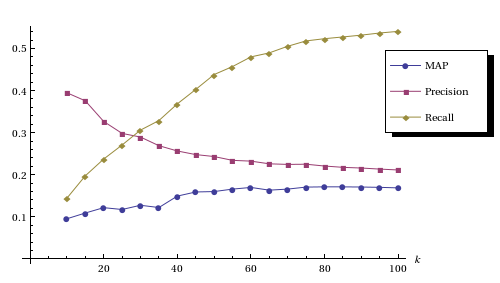
\includegraphics[scale=.65]{tfidfstats}
\caption{Search performance statistics for the systems $S_{F_{tfidf,k}}$.}
\label{filter:fig:tfidfstats}
\end{figure}

%\begin{table}
%\centering
%\begin{footnotesize}
%\begin{tabular}{l|r|r|r|r|r|r}
%\toprule
% & \multicolumn{3}{|c|}{\textbf{True positives}} & \multicolumn{3}{c}{\textbf{False positives}}\\
% \hline
%  & \textit{Abstract} & General & Specific & Abstract & General & Specific\\
%\hline
%Who & & 74& 78& &205 &133\\
%\hline
%What &84 &429 & &396 & 1890&\\
%\hline
%Where & & 37&97 & &152 &624\\
%\hline
%When & & &15 & & &21\\
%\bottomrule
%\end{tabular}
%\caption{Classification of positives for $S_{F_{tfidf,80}}$.}
%\label{filter:table:pan-shat-tfidf}
%\end{footnotesize}
%\end{table}

This section outlines the results for the systems $S_{F_{tfidf,k}}$ which consider only the top $k$ tags for each fragment where the ranking is based on the TF-IDF scores of the tags. We vary the value of $k$ from 10 to 100 with increments of 5. Figure \ref{filter:fig:tfidfstats} presents the search performance statistics as the value of $k$ varies. Not surprisingly, as the value of $k$ increases the search precision and the search recall decrease and increase, respectively. Moreover, the MAP score steadily increases until $k$ equals 80, where the maximal value is reached, and then it starts to decrease. As shown in Table \ref{filter:table:map-prec-rec}, the MAP score of $S_{F_{tfidf,80}}$ is $0.171$ which means it significantly outperforms $SE_{user}$, the systems that indexes all user tags. Indeed, the increase in search performance is 31\%. What is more important is that $S_{F_{tfidf,80}}$ slightly outperforms even $SE_{catalog}$, which until now was the best performing one and the system that we are trying to beat. This suggests that TF-IDF score is indeed a good indication of the quality of the tags and can be used to filter out the bad tags.
%Table \ref{filter:table:pan-shat-tfidf} displays the classification of the results returned by $S_{F_{tfidf,80}}$ according to the Panofsky-Shatford model. What becomes 

\subsection{Network Analysis-based filtering}
\begin{figure}
\centering
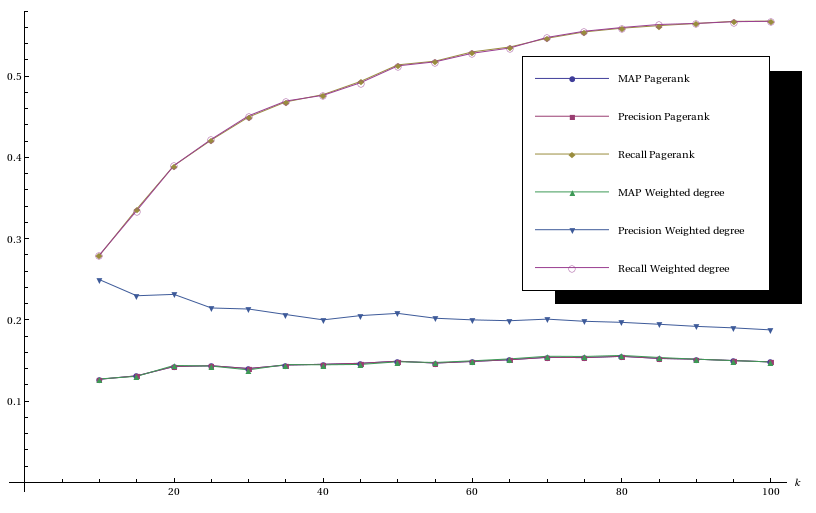
\includegraphics[scale=.45]{filter:netana}
\caption{Search performance statistics for the systems $S_{F_{pagerank,k}}$ and $S_{F_{wdeg,k}}$.}
\label{filter:fig:netana}
\end{figure}
In this section we present the results of the systems $S_{F_{pagerank,k}}$ and $S_{F_{wdeg,k}}$ which consider only the top $k$ tags for each fragment where the ranking is based on the PageRank and weighted degree centrality measures, respectively. The value of $k$ was varied from 10 to 100 with an increment of 5. Figure \ref{filter:fig:netana} summarizes the search performance statistics as the value of $k$ changes. The trends are as expected, as the value of $k$ increase the recall for both systems decreases. On the other hand, the precision drops. The MAP scores for both systems steadily increase and it reaches maximal value at 80. The values of the performance statistics for $S_{F_{pagerank,80}}$ and $S_{F_{wdeg,80}}$ are shown in Table \ref{filter:table:map-prec-rec}. As we can see both systems outperform $SE_{user}$, the system that indexes all user tags. In the case of $S_{F_{pagerank,80}}$ the improvement in terms of the MAP score is 18\% and in the case of $S_{F_{wdeg,80}}$ the improvement in terms of the MAP score is 19\%. This shows that the network centrality is a relatively good indicator of the quality. However while it is a step in the right direction, $SE_{catalog}$ and $S_{F_{tfidf,80}}$ still outperform network-analysis based filtering. Looking at the graphs in Figure \ref{filter:fig:netana} it is striking that the values for the search precision, search recall and MAP for the systems $S_{F_{pagerank,k}}$ and $S_{F_{wdeg,k}}$ as the value of $k$ changes are almost equal. In fact, the difference usually is in the second or the third decimal. This phenomenon can be explained by the structure of the networks that we construct for the fragments. Indeed, the resulting networks usually consists of many isolated well-connected network subcomponents. Consequently, the rankings produced by PageRank and the weighted degree centrality are highly correlated. The structure of the networks is an artefact of DBpedia's classification structure of the articles which is rather sparse: the set of categories is incomplete and not all article-to-category links are present. This prompts us to think that building better networks for semantic connectedness is the key ingredient. Exploiting more of the knowledge encoded in DBpedia or using a different richer knowledge source could perhaps lead to improved detection of the bad tags. 

\subsection{Player reputation-based filtering}
\begin{figure}
\centering
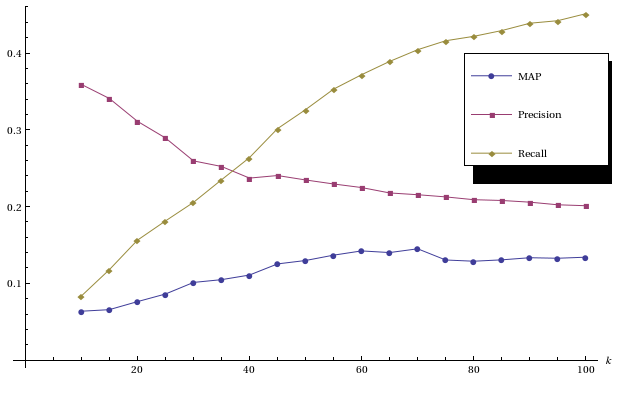
\includegraphics[scale=.5]{filter:rep}
\caption{Search performance statistics for the systems $S_{F_{prep,k}}$.}
\label{filter:fig:reppl}
\end{figure}

\begin{figure}
\centering
\includegraphics[scale=.4]{filter:repcorr}
\caption{Correlation between the reputation and the number of relevant hits for the players. The horizontal axis displays the reputation of the player in increasing order and the vertical axis shows the number of relevant videos retrieved using a tag entered by the corresponding player.}
\label{filter:fig:repcorr}
\end{figure}

This section outlines the results for the system $S_{F_{prep,k}}$ which takes only the top $k$ tags for each fragment where the ranking is based on the combination of the TF-IDF score and the reputation of the players.
As previously, the value of $k$ was varied from 10 to 100 with an increment of 5. Figure \ref{filter:fig:reppl} displays how the MAP score, search precision and search recall change as a function of $k$. The best results are achieved for $k=70$ and are displayed in Table \ref{filter:table:map-prec-rec}. As we can see there is a an improvement of $11\%$ with respect to the MAP score compared to the system $SE_{user}$ which indexes all user tags. However, the search performance of  $S_{F_{prep,70}}$ is worse for all three metrics than the system $S_{F_{tfidf,80}}$ which ranks and filters the tags based only on their TF-IDF scores. This means that considering the reputations of the players in combination with the TF-IDF ranking in this case only worsened the matters for the TF-IDF based filtering. Figure \ref{filter:fig:repcorr} shows the correlation between the reputation of the players and their success in providing tags that resulted in relevant search results. In particular, the horizontal axis shows the reputation for each of the users in increasing order whereas the vertical axis presents the number of relevant video fragments that can be retrieved using tags entered by the corresponding player. As seen, higher reputation does not entail higher success rate. In fact, many of the most  reputable players are among the ones that were the least successful. This means that computing reputation in the manner outlined above may not be the best predictor for the ability of the player to provide topically relevant tags. Alternative explanation is that there is not sufficient data available to reliably estimate the reputation of the players. Recall that 99\% of the players are registered as anonymous and the only data available for them is a single session of playing \textit{Waisda?}.

\section{Conclusions}\label{filter:sec:con}
In this study we have looked into ways we can detect and filter out bad tags and thereby improve the search performance of the video fragment retrieval based on the tags collected by the \textit{Waisda?} video labelling game.

The first direction that we took was to relax the tag verification criterion incorporated in the game. Our previous research had suggested that it is in fact rather limiting and results in omitting good tags. We made two attempts in this direction. The first attempt was to retain the tags that were entered by at least two different players. The second attempt was to keep the tags that were entered at least two times possibly by the same player. Unfortunately, neither proved to be an efficient way of detecting the good tags. The main reason for this is that even though they relax the verification criterion they are still too restricted, thus using all \textit{Waisda?} tags for search is a much better option.

The second direction that we looked into was to exploit background knowledge to filter out the bad tags. In particular, we used the GTAA thesaurus which is employed by the catalogers from the S\&V institute in the process of video annotation. The tag filtering was carried out by keeping only the tags that are present in the GTAA thesaurus. However, this turned out be a bad tag quality predictor as well. The main reason being the low overlap between the \textit{Waisda?} tags and the GTAA thesaurus. In fact, after the filtering for more than half or the queries no results were returned. This result reaffirms the conclusions from Chap. \ref{chap:kcap} about the disparity of the vocabularies used by professionals and normal users and the search gap that spawns from this disparity.

The third direction we investigated was to exploit the standard information retrieval metrics TF-IDF which reflects the importance of a word with respect to a document in a corpus of documents. The filtering is carried out for each video fragment by retaining only the top $k$ tags where the ranking is based on the TF-IDF score of the tags. It turned out that TF-IDF score is a good predictor for the quality of the tags. Indeed, for the case of $k = 80$ we obtained a search performance which is for 31\% better than the search performance of all \textit{Waisda?} tags and marginally better than the search based on the catalog data. If you recall the latter was the best performing when it comes to topical search. This means that the system $S_{F_{tfidf,80}}$ can emulate the search performance of the system $SE_{catalog}$ which is the best performing system when it comes to topical search that does not exploit user tags. 

The fourth direction we undertook was to use the social network analysis tools to characterise the quality of the tags and identify the bad ones. The filtering procedure consisted of the phases. In the first phase we constructed a network that represents the semantic connectedness of the tags in the video using DBpedia as background knowledge. Afterwards, in the second phase we ranked the tags based on their network centrality measure scores and retained only the top $k$ ones. This method of filtering proved to be an improvement over using all \textit{Waisda?} tags. However, it still performed worse than the retrieval based on the catalog data. We hypothesize that this is a consequence of the manner we build the network of semantic connectedness. Constructing a network that bears a better resemblance to the true semantic connectedness relation could yield better tag quality detection.

The last direction we examined was to exploit the reputation of the players to find the good tags. The reputation of a player was based on the positive evidence collected for that player. The positive evidence came in the form of the number of verified tags entered by that player. The reputation of the players was combined with the TF-IDF score of a given tag to compute the overall score for that tag. Unfortunately, this combined strategy yielded worse performance than TF-IDF scoring and filtering alone. This suggests that either the reputation computation mechanism we employed is not appropriate or the lack of evidence we had for the players proved to be too detrimental. In fact, the latter would be an obstacle regardless of the reputation mechanism. This could be attributed as a drawback of the design of the game which incorporated players reputation management only to a limited extend.

\chapter{Game Tags for Topical Video Search}\label{chap:topicir-filter}
\begin{quotation}
\noindent
In this chapter we continue our investigation of the usefulness of the user tags for search. Particularly, our aim is to evaluate the performance of user tags for retrieval of videos that are about a given topic i.e. \textit{topical search}. To this end, we will reuse the same methodology as in Chap. \ref{chap:ecir}, namely \textit{quantitative system evaluation} \cite{vorhees}. The results presented bellow demonstrate that raw, unprocessed game tags are not well suited for retrieving video fragments based on topic. While the search recall is satisfactory, the search precision leaves much to be desired. This is mainly caused by the presence of game tags which are not valid topical annotations. Thus, the second aim of this work is to characterize the quality of the user tags as topical annotation and to detect and filter out the non-topical ones. We explore several features of the tags which could serve as an indication of their quality as topical descriptors. Our results show that after filtering, game tags can emulate the retrieval performance of a baseline system that utilizes manually crafted metadata for search. An important consequence of this finding is that tagging games can provide a cost-effective alternative in situations when manual annotation by professionals is too costly.

This chapter is an extension of a journal article which was published as ``Topical Video Search: Analysing Video Concept Annotation through Crowdsourcing Games" in the International Journal of Human Computation 4(1), 47-66, 2017 \cite{hcj-riste}. It is co-authored with Michiel Hildebrand, Jacco van Ossenbruggen, Lora Aroyo, and Guus Schreiber.

\end{quotation}

\section{Introduction}

In the past decade audio-visual (AV) content collections have been undergoing a transformation from archives of analogue materials to very large stores of digital data accessible online\footnote{An excellent example is PrestoPRIME, \url{http://www.prestoprime.org/}, which was an European Union funded project about digitisation and preservation of the AV heritage. The consortium included the major national AV archives in Europe.}.  As the AV collection items become accessible to the wider internet audience the lack of adequate annotations is highlighted: users cannot find what they are looking for because annotations are either not present or too expert-centric --- created from the perspective of the catalogers \cite{johan-book-chap}. Video tagging games are an attempt to alleviate this problem. By engaging the internet community to tag their videos, the AV collection owners can benefit in at least two important ways. First, there is a clear cost-benefit, collecting annotations in this way is usually cheaper than using professional documentalists. Second, the game tags can help bridge the \textit{terminological gap} in search if the \textit{searchers} and \textit{annotators} originate from the same community and use similar terminology when searching and tagging. 

One of the most successful ongoing online video tagging games is \textit{Waisda?}.
The game was launched in 2009 by the Netherlands Institute for Sound and Vision (S\&V), one of the largest AV archives in Europe\footnote{S\&V manages and preserves over 70\% of the Dutch AV heritage. The collection contains more than 750.000 hours of television, radio, music and film from the beginning in 1898 until today.}.
The first pilot of the game run until January 2010 and produced over 420,000 user tags. Considering the acquired experience and insights, S\&V launched a second version of the game (see Chapter \ref{chap:waisda} for more details) which features several improvements, albeit the basic idea of the temporal tag agreement is preserved.

%\textit{Waisda?} is a multi-player game where players describe streaming video by entering tags and score points based on temporal tag agreement. The underlying assumption is that tags are faithful descriptions of the videos when entered independently by at least two players within a given time-frame.The first pilot of the game run until January 2010 and produced over 420,000 user tags. The analyses of the collected tags \cite{kcap} and user evaluations suggested potential areas of improvement. Considering the acquired experience and insights, S\&V launched a second version of the game\footnote{The game is deployed online and can be accessed at \url{http://woordentikkertje.manbijthond.nl/}. The source code is published as open-source under the GPL licence and can be downloaded from \url{https://github.com/beeldengeluid/waisda}.} which features several improvements, albeit the basic idea of the temporal tag agreement is preserved. 
%Figure \ref{filter:fig:game} shows the game page of \textit{Waisda?}. It contains a video player and below it a text-entry field. When the player enters the game page the video automatically starts playing, the text-entry field receives focus, and the player can start entering tags. The right side of the page contains the score board. It consists of the current score of the player, the current rank and a listing with all tags entered by the player. The tags are displayed with their score and an icon indicating the tag type (person, location etc.).
%\begin{figure}
%\centering
%\includegraphics[scale=.35]{game.png}
%\caption{Screenshot of the \textit{Waisda?} game page with public domain video clip from Preligner Archives.}
%\label{filter:fig:game}
%\end{figure}

The second version of \textit{Waisda?}\footnote{At the time of writing the second version of the game has been discontinued. S\&V is deploying (still under development) a third installment of the game available at \url{http://waisda.beeldengeluid.nl/}. S\&V intends to integrate \textit{Waisda?} more tightly in their internal workflows and to use it to collect tags for the items in their online collection \url{http://in.beeldengeluid.nl/}.} is a mature, production-grade, customizible GWAP with diverse usage. 
It is included\footnote{\url{http://labs.europeana.eu/apps/waisda-floss}} as a showcase in the Europeana\footnote{Europeana is an internet portal that provides multi-lingual access to millions of books, paintings, films, and archival records that are part of the European cultural heritage. More than 2,000 institutions across Europe have contributed to the project.} internet portal (see Section \ref{sec:waisda-europeana} for more details). \textit{Waisda?} has also been deployed and incorporated in Spotvogel\footnote{\textit{Spotvogel} (\url{http://spotvogel.vroegevogels.vara.nl/}) which translates to \textit{mocking bird} from Dutch, was a \textit{Waisda?} deployment by the Dutch broadcaster VARA (\url{http://www.vara.nl/}) and the S\&V institute with the aim of collecting user tags for the footage from the Dutch television program \textit{Vroege Vogels} (\url{http://vroegevogels.vara.nl/}). The game run for 6 months in 2013 and was nominated for Dutch Game Awards 2013 \url{http://www.dutchgameawards.nl/2013/spotvogel/}, note that the link is in Dutch.} (see Section \ref{chap:waisda:spotvogel} for more details). In the former the internet users tag archival footage from the European cultural heritage and in the latter they identify occurrences of wildlife in footage. These are two relatively different domains yet \textit{Waisda?} was fitted to them seamlessly. This is due to the simple design of the game and the unconstrained way the tags are entered --- the players get a small set of instructions and then are free to enter whatever they please. This is a double-edged sword. On the one hand, the entry barrier for the players is low and the target audience is wide as no specific skills are needed. On the other hand, the open-ended way the tags are entered may be overwhelming in the fast-pased setting of the game and players may succumb to entering low quality tags which lack descriptive power just to reach consensus with other players and win points. In this study we perform a qualitative analysis to investigate this issue.

The cost-effectiveness of \textit{Waisda?} versus manual annotation by professionals comes with a caveat: successful deployment of a GWAP is no small feat. Attracting new players and keeping them engaged over time is vital for success and requires continuous publicising efforts. The empirical evidence collected from both \textit{Waisda?} pilots supports this claim. On both occasions the bulk of the tags was accumulated during periods when there was an active campaign for promoting the game. Targeting the fanbase of the TV series via various channels (e.g. TV series website, social media, etc.) has proved to be a successful strategy for attracting new players. Player's engagement is sustained with in-game mechanisms such as leaderboards to honour the best players and motivate the others, and with time-limited contests offering awards for the top performers. Planning and executing activities like these is certainly costly, however in the case where the growth rate of AV collections is ever increasing, these costs will be outweighed by the costs of manual annotation. This is one of the lessons learned from the \textit{Waisda?} project.


The second version of the game has amassed more than 710,000 user tags. The number of unique tags is 71,448 and each of the top five most-tagged videos has more than 3,600 tags ascribed to it which amounts to an average tag density of more than 13 tags per second. This is a substantially higher number than the number of tags assigned by professional catalogers, typically 10-20 tags per video. However, are all these user tags of any use? Does this overwhelming quantity implies quality? In Chapter \ref{chap:ecir} we demonstrated that the \textit{Waisda?} tags can indeed be successfully exploited for retrieving video fragments that feature \textit{visual appearances} of objects of interest (persons, objects, etc.) \cite{ecir}. Our results showed that \textit{Waisda?} tags excel at this kind of \textit{visual instance search}, outperforming the closed captions and annotations created by professionals. 

In this study we wish to understand whether the fast pace of \textit{Waisda?} forces players to have tunnel vision about the content of the video and tag predominately non-topical aspects.
Previous analysis performed by a senior cataloger from S\&V ruled the game tags to be limited in scope, referring mainly to things seen or heard on the screen \cite{waisda-lotte}.
However, we hypothesize that players do describe topics and topical tags are present albeit buried under the myriad of non-topical tags. The first research question, therefore is
\begin{itemize}
\item[RQ1] Do players enter tags which describe the topics of the videos?
\end{itemize}
In the context of topical video search, the presence of non-topical tags, which do not refer to the topics covered in the video, can lead to false positives. For example, if a video $v$ has a tag $t$ ascribed to it and $t$ does not refer to the topics covered in $v$. If a searcher is interested in videos that are about $t$ and uses $t$ as a search term the video $v$ will be incorrectly retrieved. Thus, it is important to know whether a tag is non-topical and ignore it in the retrieval process to eliminate its negative influence on the search results. Our second research question, therefore is
\begin{itemize}
\item[RQ2] Can the access to videos based on topic be improved by detecting and filtering out the non-topical game tags?
\end{itemize}

The rest of the chapter is structured as follows. In Section \ref{sec:topicir-filter:relatedwork} we discuss related work. Section \ref{sec:topicir-filter:approach} outlines our approach. In Section \ref{sec:topicir-filter:video-metadata-collection} and \ref{sec:topicir-filter:eval-ds} we describe the collection of video fragments and the evaluation dataset, respectively. Section \ref{sec:topicir-filter:all-tags} presents the findings with respect to the effectiveness of the user tags for topical search. This sets the baseline for the remainder of the study. In Section \ref{sec:topicir-filter:filtering} we outline a number of tag filters and evaluate their effectiveness for eliminating non-topical tags. Section \ref{sec:topicir-filter:con} presents the conclusions from the study.

\section{Related Work}\label{sec:topicir-filter:relatedwork}
\paragraph{User annotations for search.} Search based on user-generated metadata, in particular folksonomies, has been studied before. Morrison compared web search performance of folksonomies from social bookmarking web sites against search engines and subject directories \cite{morison}, showing that search engines had the highest precision and recall rates. Folksonomies, however, performed surprisingly well. In fact, user tags show promise to alleviate the vocabulary mismatch problem for search: bridging the gap between user queries and metadata used for retrieval \cite{vocprob}. Indeed, Geisler and Burns state that YouTube tags provide added value for search, because 66\% of them do not appear in  other metadata \cite{youtube}. Heymann et al. investigated a large-scale sample of forty million bookmarks from the social bookmarking site del.icio.us and found that in 20\% of the cases user tags do not occur in the page text, backlink page text, or forward link page text of the pages they annotate. Studies in \cite{Bischoff:2010:BGT:1833903.1834001,Halvey:2007:AOV:1286240.1286301,journals/jasis/Rorissa10,Yanbe:2007:SBE:1255175.1255198} investigate this phenomenon across multiple domains and multimedia resource types and identify the gaps between the tag space and the querying vocabulary. The common conclusion is that user tags can improve search by bridging the vocabulary gap. 

Studies reported in \cite{Bischoff:2008:TUS:1458082.1458112,Sun:2010:QTR:1873951.1874029,Marshall:2009:NBN:1555400.1555438} take a more critical stance. They conclude that while overall user tags improve search, not all tags are suitable for retrieval. In fact, Marshall \cite{Marshall:2009:NBN:1555400.1555438} even suggests that tags  may be less effective descriptors for image retrieval, classification, and description than other forms for descriptive metadata such as title and narrative captions. This hints that a characterization of the quality of the tags is needed to filter out the tags that are not suited for retrieval. This is one of the aspects that our study addresses. 

Another line of research is exploiting the tripartite structure ($Users \times Tags \times Resources$) of folksonomies to improve search \cite{Hotho:2006:IRF:2094613.2094652,Bao:2007:OWS:1242572.1242640}. Alternatively, the semantics of tags can be grounded in some lexical sources and the grounded tags utilized for improving search. For example, Hildebrand et al. proposed and investigated a semi-automatic process of assigning explicit meaning to user tags for video by linking them to concepts from the Linked Open Data cloud \cite{michiel}. Gligorov et al. evaluate the performance of user tags collected with a GWAP for retrieval of video segments that depict particular concept of interest (person, object, etc.) \cite{ecir}.

\paragraph{Quality and Refinement of Annotations.} There is a substantial body of research into the refinement and quality assessment of annotations of still images. Lee at al. propose a tag refinement technique that aims at
differentiating noisy tag assignments from correct tag assignments \cite{Lee:2010:TRI:1890924.1891010}. Each tag is assigned a probability of being noisy based on the visual similarity of the images and tag co-occurrence statistics. Tags with a probability above a threshold are discarded as noisy. 

In \cite{Truong:2012:CSK:2324796.2324808,Li:2008:LTR:1460096.1460126} neighbour voting schemes for determining the tag relevance are explored. In this approach, a tag is considered more relevant to the image it is ascribed to, also known as the seed image, if the tag is also used to annotate the neighbouring images. The neighbourhood relation is defined in terms of the visual similarity among images. Lee at al. expand the approach by not only considering the visually similar images, but the dissimilar images as well, thus providing negative examples \cite{Lee:2012:TDE:2390876.2390880}. Kennedy at al. exploits visual similarity among images in a sense that tags ascribed to images by the creators of the image are used as seed annotations and also attached to visually similar images \cite{Kennedy:2009:RTU:1631135.1631139}. Zhao at al. propose a data-driven method to automatically determine the relatedness between a tag and the image's visual content taking into consideration the tag co-occurrence and the visual similarity among images \cite{Zhao:2010:TRV:2174490.2174571}.

Probabilistic methods that exploit random walk based techniques have also been explored \cite{Wang:2006:IAR:1180639.1180774,Liu:2009:TR:1526709.1526757,Li:2012:TRP:2382336.2382380}. These methods produce a ranking of the tags according to their relevance with respect to the image with which they are associated. The tag relevance estimations are computed as the stationary or the convergence probabilities of  a random walk processes. Notable example of this approach is the PageRank algorithm \cite{journals/corr/abs-1012-4872,10.4137/GRSB.S702,junker2008analysis}. Another group of methods exploit background knowledge (such as the lexical database Wordnet and a massive corpus indexed by Google) to perform the refinement of the image annotations \cite{Jin:2010:KBI:1731523.1731529,Wang:2007:RIA:1282280.1282343}. The semantic relations encoded in Wordnet and the semantic similarity quantified by the Google-based measures like the Normalized Google Distance \cite{DBLP:journals/corr/abs-cs-0412098} provide contextual evidence for the relationship among the annotations. This evidence is then used as an input for machine learning algorithms which give the final word for the quality of the annotations. 

\paragraph{Games With a Purpose (GWAPs)}
GWAPs are a human-based computation technique in which humans solve tasks, too difficult for computers, in a game setup which provides entertainment for the players. The predecessor of all GWAPs is the ESP game designed by von Ahn and Dabbish \cite{CHI2004:vonAhn}, which harnesses human abilities to label images. The general idea of the ESP game is that two players who can see the same image try to come up with matching tags. The players are paired up randomly without any means of communication. Therefore, when players agree on a tag it is a strong indication that the tag is a valid descriptor of the image. In \cite{vonAhn:2008:DGP:1378704.1378719} von Ahn and Dabbish generalize the design principles of the ESP game into a conceptual framework for designing GWAPs. Given a problem which is hard or impossible to solve by computer the framework provides high-level guidelines and principles for transforming the problem into GWAP that solves it. Following the ESP game, many GWAPs were designed that tackle problems from various domains. \textit{Peekaboom} is a GWAP in which players identify and locate objects in images \cite{vonAhn:2006:PGL:1124772.1124782}. The output of the game is precise location information and other useful information which can be used to train computer vision algorithms. Several GWAPs have been designed for collecting or validation of common sense knowledge. \textit{Verbosity} is a GWAP \cite{vonAhn:2006:VGC:1124772.1124784} which addresses the problem of creating a database of `common-sense facts', statements about the world known to most people. Similarly, \textit{Common Consensus} is a GWAP that aims at collecting a database of human \textit{goals} \cite{lieberman2007}. \textit{Top10} and \textit{Pirate \& Ghost}\cite{DBLP:conf/aaaifs/ChangCH10}, on the other hand, are GWAPs that deal with the problem of verification of the common sense assertions of the form \textit{concept} $\rightarrow$ \textit{relation} $\rightarrow$ \textit{concept}. Another area where GWAPs are applied is collecting visual data for real world locations. \textit{EyeSpy} is a GWAP in which players contribute photos or textual data about geographic locations \cite{Bell:2009:ESN:1518701.1518723}. The collected data is subjected to in-game validation by other players and once validated can be used for navigation tasks. \textit{PhotoCity} is another GWAP where players contribute photos of real world locations in urban areas \cite{Tuite:2010:RWB:1822348.1822379,Tuite:2011:PTE:1978942.1979146}. The ultimate goal is to use the collected photos to build detailed 3D models of real world places varying over time. GWAPs have also been applied in the music and art domains. \textit{TagATune} \cite{Law2007,Law:2009:INM:1518701.1518881} and  \textit{Listen Game} \cite{Turnbull07agame-based} are GWAPs where the aim is to collect annotations for music pieces. 
\textit{Artigo}\footnote{\textit{Artigo}, \url{http://artigo.org}, is a game platform for artwork annotation as well as artwork semantic search engine in German, English, and French founded in 2008. According to \cite{PMS-FB-2015-1}, thanks to a good media coverage over several years, the German version of ARTigo has a sufficient number of regular players.} is a game platform that offers six GWAPS for annotating artworks \cite{PMS-FB-2013-3}. Three of the games \textit{Artigo game}, \textit{Artigo Taboo}, and \textit{TagATag} are variations of the ESP game. \textit{TagATag} includes a more challenging aspect where players are tagging pairs consisting of an image and a tag. The resulting tags describe relationships between the members of the pair(the image and the tag). The other three game of the platform, \textit{Karido}, \textit{Artigo-Quiz}, and \textit{Combino} are designed to complement the data collected with the first three ESP-like games. In \textit{Karido} \cite{DBLP:conf/cgames/SteinmayrWKB11} the process of annotation is carried out as a guessing game where one player is trying to guess  \textit{goal image} out of set of images. Second player tries to help the first player by providing description of the image. If the first player correctly guesses the goal image then the description is valid annotation with high probability. The aim of the \textit{Combino} game is to collect semantically more complex multi-word tags \cite{PA_Florian.Stoerkle}.
Semantic web is another area for application of GWAPs. \textit{OntoGame} is a series of GWAPs that aims to cover the complete Semantic Web life-cycle: building and maintaining ontologies, alignment of ontologies, and semantic annotation of data \cite{Siorpaes:2008:GPS:1373102.1373155}. Building and maintaining ontologies is carried out with the \textit{OntoPronto} GWAP \cite{thaler2012experiment}, alignment of ontologies is achieved with the \textit{SpotTheLink} GWAP \cite{DBLP:conf/wm/ThalerSS11}, and semantic annotation of resources is done with the \textit{OntoTube} and the \textit{OntoBay} GWAPs. \textit{GiveALink Slider} and \textit{Great Minds Think Alike} are two more GWAPs that address the problem of collecting reliable semantic annotations \cite{Weng11cgames}. Another area where GWAPs are applied is linguistics. \textit{Jinx} is a GWAP that tackles the problem of word sense disambiguation \cite{Seemakurty:2010:WSD:1837885.1837905}. \textit{Borsa Parole} and \textit{Poker parole} are GWAPs that aim at collecting linguistic data \cite{PMS-FB-2013-4}. In \textit{Borsa Parole} word phrases and their characteristics are collected from the user community. \textit{Poker parole} aims at collecting meta-data about the data collected in \textit{Borsa Parole} i.e. players form conjectures about the word phrases and their characteristics. Other notable GWAPs are \textit{Odd Leaf Out} which addresses the problem of misclassified leaf images \cite{DBLP:conf/socialcom/HansenJLBPRS11} and \textit{Polarity} which deals with collecting attributes and attribute values for resources \cite{law.cvpr11ws}. Pearl and Steyvers in \cite{Pearl:2010:IEI:1860631.1860640} outline a GWAP-based methodology for identifying emotions, intentions, and attitudes in text. Kneissl in \cite{ediss16841} studies how GWAPs and more generally crowdsourcing can be used in the field of e-learning.

Important area of research is on the limitations of ESP-like games. Weber at al. demonstrated that the ESP game in its original design encourages players to enter `obvious' or predictable tags \cite{DBLP:conf/chi/RobertsonVW09}. Weber at al. built a probabilistic language model which using only the already assigned tags for the image and without any knowledge about the image was able to predict with high probability\footnote{Even without any understanding  of  the  actual  image,  the  probability of agreement with randomly assigned human partner on a label was 69\% for all images, and 81\% for images which have at least one tag assigned to them.} what the new tags added by players will be. Jain and Parkes provided a game-theoretic explanation for this observation \cite{Jain:2013:GAE:2399187.2399190}. Their game-theoretic model of the ESP game indicated that from the players' point of view it is more beneficial if they focus on more obvious (low-effort) tags.

\section{Approach}\label{sec:topicir-filter:approach}
To answer the research questions stated above we use a quantitative system evaluation methodology \cite{vorhees} which requires an evaluation dataset that consists of three components: a document collection (in our setting video fragments tagged by players in \textit{Waisda?}), a set of representative queries, and relevance judgements. To evaluate the performance of a search system, the query set is run against the system and the retrieved results are graded w.r.t the relevance judgements\footnote{Relevance judgments give binary (yes/no) answer as to search result is relevant to the query. Thus, the retrieval process was fully automatized.}. The search performance or the search system is then quantified by search performance metrics such as Mean Average Precision (MAP), Recall,
Precision, etc. Central to this evaluation methodology is the creation of the relevance judgements which plays the role of \textit{gold standard}. In the making of the gold standard we exploit in-house annotations created by the broadcaster which describe the main topics in the video. More precisely, we deem a video to be relevant for a query if the query concurs with at least one the topics (annotations) of the video (see Sec. \ref{filter:ground-truth}).

Our study is divided in two parts. In the first part we address the first research question: do players enter topical tags and in effect how suited are the game tags for topical search. To this end, we create four search systems, each exploiting different metadata. We run each system against the evaluation dataset and carry out comparative analysis of their retrieval performance. The first and the second system use all game tags and \textit{verified}\footnote{Tags entered by at least two players within a time interval of 10 seconds.} only game tags, respectively. The third system is our baseline and exploits the in-house catalog metadata --- it is an approximation of the present search functionality. The forth system combines all game tags and the in-house catalog metadata. By comparing the first and the second system against the baseline system, we deduce how suited the game tags for topical search are on their own, and see if they could replace the need for the current expensive cataloguing practice. By comparing the forth system with the baseline, we infer whether the game tags provide added value on top of the existing catalog metadata. 
To get a better qualitative insight of what happens under the hood, we carry out an analysis of example false/true positives. We classify the game tags according to the Panofsky-Shatford scheme \cite{laurapaper} to establish which parts of the video content are described by the tags. The aim is to derive insights about users' tagging practices that are associated with ascribing topical tags. 

In the second part we address the second research question: we investigate several ways to detect and filter out non-topical tags with the goal of improving topical search performance. In particular, we take tag features such as TF-IDF score and player's reputation and derive a binary yes/no decision as to whether to retain the game tag or drop it. Each filtering method yields a subset of all game tags. To judge how well each of the filtering methods work we build a search system for each of them which uses the corresponding subset of all game tags as input for search. Moreover, to see how well the filtering methods work together with the existing catalog metadata we build a search system for each of them which uses the corresponding subset of all game tags and the catalog metadata as input for search. The search performances of these systems are compared to the baseline system from the first part of the study (see Sect. \ref{sec:topicir-filter:filtering} for more details).

When comparing the performance metrics of any two systems, to assess whether the difference is statistically significant we use the student's paired t-test at 0.01 level of significance as suggested by \cite{stat-sig}.

\section{Experimental Data}
In this section we describe the data and the evaluation dataset used in this study. More precisely, Section \ref{sec:topicir-filter:video-metadata-collection} outlines the metadata that we exploit for search and Section \ref{sec:topicir-filter:eval-ds} describes in more detail the evaluation dataset.

\subsection{The MBH Video and Metadata Collection}\label{sec:topicir-filter:video-metadata-collection}
In the second pilot, \textit{Waisda?} was used to % is in its second release. In this release the collection of fragments that are tagged by players originates from 
tag fragments from the popular Dutch TV program `Man Bijt Hond' (MBH, English: `Man Bites Dog') produced by the Dutch broadcaster NCRV\footnote{\url{http://www.ncrv.nl/}}.  MBH is a humoristic TV show that focuses on trivial, everyday news and ordinary, unknown people.  Every episode consists of 7-8 unrelated, self-contained fragments where each fragment topically comes under a recurring heading. Players in \textit{Waisda?} tag these fragments.  The entire video collection to which we have access has 11,109 fragments from episodes aired in the last 11 years.

In addition to the video fragments, we have access to four types of descriptive metadata that we use as input for search in this study:
\paragraph{\textbf{\textit{Waisda?} game tags.}} We consider the collection of all user tags acquired with \textit{Waisda?} during the first five months, starting from October, 2011. In this period 436,456 different tag entries were assigned to 2,192 video fragments by roughly 24,000 players. The number of unique user tags exceeds 47,000. Each tag entry is associated with the point in time --- relative to the beginning of the fragment --- when the tag was entered. Additionally, each tag entry is marked as `verified' or not based on whether the tag was entered by at least two players within a time interval of 10 seconds.
As the game is advertised only in Dutch media and the material being tagged is exclusively in Dutch, the language of almost all tags is Dutch. The average number of tags per video is 199. Approximately 55\% of all user tags ($\approx$ 243,000) are `verified' and the number of unique verified tags is 12,861. The average number of verified tags per video is 111.
\paragraph{\textbf{NCRV tags.}} NCRV, the broadcaster, maintains an in-house collection of tags % that describe their video material. The purpose of these tags is 
to facilitate web access to MBH fragments via search and browsing. In contrast with \textit{Waisda?} tags, NCRV tags are not time-based, meaning they are not linked to a particular time-point in the video, and generally cover only the prevalent topics. The average number of NCRV tags per video is 11. Thus they are usually much scarcer than the game tags.
\paragraph{\textbf{NCRV catalog data}.} Along with the curated NCRV tags, each MBH fragment has a short textual description, usually one paragraph, and a title. We consider the collection of all titles and textual descriptions (i.e. catalog data) as another metadata type that will be used in the study.
\paragraph{\textbf{Captions}.} % Yet another metadata type we make use of is the subtitle files associated with the video fragments. 
Closed captions are textual versions of the dialogue in films and television programs for the hearing impaired, usually displayed at the bottom of the screen. Each dialogue excerpt is accompanied with time-points --- relative to the beginning of the video --- when the dialogue excerpt appears on and disappears from the screen. We use captions  obtained from S\&V\ that cover most of the MBH episodes aired in 2010 and 2011 which amounts to a total of 897 fragments. 
 
\subsection{Evaluation Dataset}\label{sec:topicir-filter:eval-ds}
In this section we describe the three components of our evaluation dataset: set of queries, set of video fragments, and relevance judgements. The evaluation set is publicly available online at \url{https://goo.gl/zXZeYq}.
\subsubsection{Query set}
We will reuse the same set of queries from a previous evaluation of the \textit{Waisda?} tags for \textit{visual} search \cite{ecir}. Here by visual search we mean \textit{keyword} search where the goal is to retrieve videos that visually depict the object/artifact of interest. The query set consists of fifty queries that were sampled from user query logs of the TV series' web site. The sampling procedure involved grouping the queries into three classes based on their frequency in the logs: \textit{high}, \textit{mid}, and \textit{low} frequency class. Each of the three classes were then filtered to remove bias and to ensure fair comparison of the retrieval performance of the metadata types. The top-ranked 12, 19, and 19, queries, w.r.t. frequency, from the high, mid, and low frequency class, respectively, comprise the final query set. The exact details of the sampling procedure can be found in \cite{ecir}. An example of a high-frequency query is \textit{Mandy} which is the main character in one of the rubrics in the MBH show. On the other hand, an example of a low-frequency query is \textit{Friesland} which is a region in the Netherlands and the filming location of one of the rubrics in the MBH show.

An objection may be raised for reusing the same queries from the visual search study, where the goal is to retrieve videos that \textit{depict the artefact} specified by the query, for topical search, where the goal is to retrieve the videos that are \textit{about the topic} specified by the query. However, most queries can refer both to an object/artefact appearing in the video or to one of the topics the video is about. For example, consider the query \textit{horse}. A video may depict a horse as part of the scenery and this would qualify it as a relevant result for visual search where we might be looking for stock footage containing horses.  Another video may be about equines and therefore be a relevant result for topical search on the topic \textit{horses}.
In fact, the query selection procedure used in the visual search study \cite{ecir} was oblivious about the searcher's intent behind the queries, be it visual, topical or something else. Only after the queries were selected a visual search interpretation was assigned to them and the gold standard was created accordingly. In the same manner, in this study we give the queries a topical interpretation which is embodied in the gold standard (see Sect. \ref{filter:ground-truth} below). Figure \ref{filter:fig:reljud} shows the number of topically relevant videos per query as judged by the gold standard. As seen, for every query there is positive number of relevant videos which means all queries can be interpreted topically.

\subsubsection{Video fragment set}
The set of fragments for this particular experiment is selected from the MBH fragments tagged in \textit{Waisda?}, described in more detail in Section \ref{sec:topicir-filter:video-metadata-collection}. For a fair comparison of the search performance, we select a subset from the entire collection of fragments. The selection criterion is as follows: only fragments that have at least one verified \textit{Waisda?} tag ascribed to them are considered. The resulting collection contains 2,562 fragments with accumulative duration of almost 123 hours of video material.
The average fragment length is approximately 2.9 minutes and the median is 3.2 minutes. The duration of the shortest and the longest fragment in our collection is 0.1 and 25 minutes, respectively. The total number of user tags, verified user tags, and NCRV tags ascribed to the videos of this collection is 591,468, 355,522, and 28,248, respectively. Thus, the average number of user tags, verified user tags, and NCRV tags per fragment is 231, 139, and 11 respectively.


\subsubsection{Ground Truth}\label{filter:ground-truth}

\begin{figure}
\centering
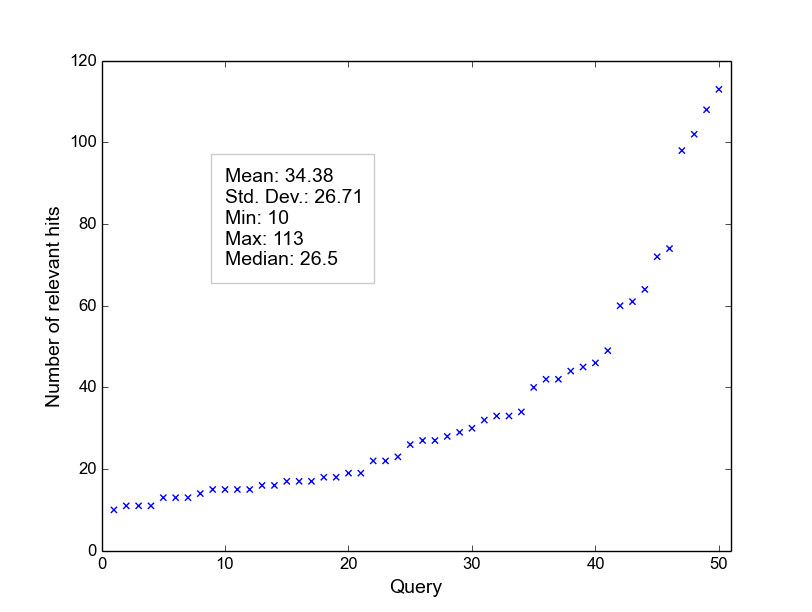
\includegraphics[scale=.4]{reljud.png}
\caption{Number of relevant hits per query in increasing order.}
\label{filter:fig:reljud}
\end{figure}
As we said earlier, % in Section \ref{sec:topicir-filter:video-metadata-collection},
NCRV tags are in-house tags that describe the topics of the fragment with which they are associated.
We consider the NCRV tags as the ground truth about what topics are covered by the fragments.
With this in mind, given a query $q$ and a fragment $f$, we deem $f$ to be topically relevant for $q$ if there is an NCRV tag that is equal with $q$, a synonym of $q$, or a hypernym of $q$. $Y$ is a hypernym of $X$ if every $X$ is a $Y$, for example \textit{canine} is a hypernym of \textit{dog}. Hyperonymy is a transitive relation \cite{wordnet}. More formally, the topical relevance relation is defined as follows
\begin{eqnarray}\label{ground_truth}
Topical\_Relevance &=& \{(q,f)~|~\exists t~(t \in NCRV(f)~\wedge \nonumber\\ 
				  &&(lower(q) = lower(t)~\vee \nonumber\\
				  &&~synonym(lower(q), lower(t))~\vee \nonumber\\
				  &&~hypernym(lower(t), lower(q))))\}
				  \label{top_rel_def}
\end{eqnarray}
where $NCRV(f)$ is the set of all NCRV tags associated with the fragment $f$, $lower(\cdot)$ is the lower case string function, $synonym(w_1, w_2)$ is a binary predicate which is true iff $w_1$ and $w_2$ are synonyms, and $hypernym(w_1, w_2)$ is a binary predicate which is true iff $w_1$ is a hypernym of $w_2$. Figure \ref{filter:fig:reljud} shows the number of relevant fragments in our collection for the queries in the dataset along with additional descriptive statistics. As seen, the median and the average number of relevant hits for a query is approximately 27 and 34, respectively. The lowest number of relevant hits for a query is 10 whereas the highest is 113.

The NCRV tags were primarily created to be used for searching and browsing on the TV-show website by the online community. The tags are displayed prominently on the website's UI which enhances the \textit{social proof} effect \cite{Floeck:social-proof,golder2006usage}, thus many of the tags are incorporated in the terminology of online community. In fact, our chosen query set belongs to the intersection between the NCRV tags and the online community's search terminology as witnessed by Fig. \ref{filter:fig:reljud}. 
As implied by the definition (\ref{top_rel_def}) and seen in Fig. \ref{filter:fig:reljud}, for every query in the query set there is at least one video annotated with the same NCRV tag.
This is sufficient for our narrower aim to determine the relevance for this particular query set and not for \textit{any} query in general. In other words, the mismatch between the NCRV tags and online community's terminology has no impact on the derived relevance judgements for our query set.

Note that while the NCRV tags are currently used by the broadcaster on the TV-show website, there is no guarantee that they, when used as described above, form a complete and accurate ground truth for topical search. We choose this set-up  because the alternative scenario, creating a dedicated topical search ground truth for a limited subset ourselves, would have resulted in a much smaller data set.

We considered variation of definition \ref{ground_truth} where we defined the topical relevance relation only by considering case-insensitive string comparison (omitting synonyms and hyponyms). Even with the modified definition the general conclusions from Sections  \ref{filter:sec:ses} and \ref{sec:topicir-filter:filtering} below remained the same;  while the retrieval metrics of the systems (given by Tables \ref{topicir:table:map-prec-rec} and \ref{filter:table:map-prec-rec}) varied slightly the ordering did not change and the differences remained statistically significant.

\section{Evaluation of Game Tags for Topical Video Search} \label{sec:topicir-filter:all-tags}
In this section we will evaluate the effectiveness of the \textit{Waisda?} tags for topical video search. The results obtained here will serve as a starting point for comparison in the subsequent sections where we will try to improve the retrieval effectiveness of the \textit{Waisda?} tags by filtering those that are irrelevant as topical descriptors.

\subsection{Game tags vs. catalog data}\label{filter:sec:ses}
To address the first research question stated above we created four search engines. Each of them utilizes the same state-of-the-art probabilistic ranking function BM25 and the only variation among them is the metadata they index and use as input for search. Consequently, differences in retrieval performance are attributed solely to the data. We evaluted search engines that index:

\begin{tabular}{lll}
 1. & $SE_{user}$  & all \textit{Waisda?} tags \\
 2. & $SE_{vuser}$& only verified \textit{Waisda?} tags \\
 3. & $SE_{catalog}$&  NCRV catalog data \\
 4. & $SE_{user+catalog}$&  catalog data and all \textit{Waisda?}  tags \\
\end{tabular}

We did not consider using captions for search because we only have them available for a small subset of MBH fragments. If we would have used them in the study, we would have had to settle for much smaller evaluation collection of fragments. Naturally, we did not use the NCRV tags either, since we used them as ground truth for topical relevance.

As said, the combinations of metadata types that are indexed by the various systems are strategically chosen so that the resulting performance metrics from the evaluation dataset will provide answers to the first research question. We compare the performance of $SE_{user}$ against $SE_{catalog}$ to evaluate the performance of the game tags alone when compared to the catalog metadata. By comparing $SE_{user}$ against $SE_{user+catalog}$ we see if the performance of the catalog metadata can be further improved by adding the game tags. Furthermore, we check whether the performance of the game tags can be improved by just using the verified tags ($SE_{user}$ versus $SE_{vuser}$).

\subsection{Results}\label{sec:topicir:results}

\begin{table}[tb]
\centering
\begin{footnotesize}
\begin{tabular}{l|l|l|l}
\toprule
System & MAP & Precision & Recall \\
\hline
$SE_{user}$ & $0.131^{\approx \uparrow}$ & $0.16^{\approx \downarrow}$ & $0.589^{\approx \uparrow}$ \\
\hline
$SE_{vuser}$ & $0.081^{\downarrow \approx}$ & $0.193^{\uparrow \approx}$ & $0.286^{\downarrow \approx}$ \\
\hline
$SE_{catalog}$ & $0.168^{\uparrow \uparrow}$ & $0.438^{\uparrow \uparrow}$ &	$0.291^{\downarrow \uparrow}$ \\
\hline
$SE_{user+catalog}$ & $0.151^{\uparrow \uparrow}$ & $0.17^{\uparrow \downarrow}$ & $0.654^{\uparrow \uparrow}$ \\
\bottomrule
\end{tabular}
\caption{MAP/Precision/Recall scores for the search engines. $\uparrow$, $\downarrow$, and $\approx$ indicate if a score is significantly better, worse, or statistically indistinguishable from the MAP scores of $SE_{user}$ and $SE_{vuser}$, in that order.}
\label{topicir:table:map-prec-rec}
\end{footnotesize}
\end{table}

Table \ref{topicir:table:map-prec-rec} summarizes our findings; the detailed precision and recall metrics for each query can be found in appendix \ref{appen:prec-recall-topical}.
Compared to the previous study (reported in Chapter \ref{chap:ecir}) where we looked at visual relevance, the results for topical relevance are dissapointing. The search performance of game tags ($SE_{user}$) is 28\% below that of the NCRV catalog data ($SE_{catalog}$). Combining the game tags with the catalog metadata does not help either: $SE_{catalog}$ is better than $SE_{user+catalog}$ by 11\%. 
The good news is that $SE_{user}$ outperforms $SE_{catalog}$ on recall: the poor MAP score is largely due to the low precision, only 0.16.

The results are even worse for the verified user tags. While they yield only marginally better search precision, their recall is far worse (see Table \ref{topicir:table:map-prec-rec}). Consequently, $SE_{user}$ outperforms $SE_{vuser}$ by 62\% which suggests that considering all tags is better for topical search than limiting the scope only to verified tags.

In conclusion, the good recall of the game tags does not outweight the low precision. The latter is caused by \textit{Waisda?} tags that match the query but are associated with fragments that are not considered topically relevant. Below, in Section \ref{sec:topicir-filter:filtering}, we attempt to detect and filter out these tags to improve the search performance.

\subsubsection{A Closer Look on Verified Tags}\label{topicir:qual-ana}
The results presented in the previous section suggest that verified tags leave much to be desired when it comes to topical search. To get a better qualitative insight of what happens behind the scenes we carry out an analysis of samples of the results returned by the system that indexes the verified \textit{Waisda?} tags. Our hypothesis is that the tags referring to objects that are visually depicted in the videos are the leading reason for the poor retrieval performance. To test this we analyse a subset of the \textit{false positives} and a subset the \textit{true positives} returned by $SE_{vuser}$. For each query we consider all returned videos--- either true or false positive --- for which captions are available. The subject of the analysis is the tag that caused a given video to be returned for a given query.

First, we classify each tag in the samples into three categories based on the content component --- audio, visual, or both --- it refers to (note that the classification was carried out by a single rater). Tags that refer to concepts that are visually depicted but are not mentioned in the dialog are classified as \textit{only visual}. Tags that are mentioned only in the dialog are classified as \textit{only in captions}. The third category contains the tags that refer to concepts that are both visually depicted and present in the dialog. Second, for each of the categories we compute the average TF-IDF (Term Frequency - Inverse Document Frequency) for the tags in that category. TF-IDF is a numerical statistic which reflects how important a term is to a document in a collection or corpus \cite{tfidf1,tfidf2}. In our context, the TF-IDF score of a tag reflects the relevance of the tag for the associated fragment where the fragments are represented as bags of all tags ascribed to them.  The average TF-IDF score of a category is an indicator of the average relevance of its members relative to the other categories. Lastly, to establish what aspects of the video content the tags from our samples are describing we classify them according to the Panofsky-Shatford model \cite{laurapaper}. This model divides the descriptions into three levels: \textit{general} (generic things in the video), \textit{specific} (specific things), and \textit{abstract} (symbolic things). Each of the levels is further broken down into four facets: \textit{who}, \textit{what}, \textit{where}, and
\textit{when} producing the Panofsky-Shatford 3x4 matrix. There are alternative tag classification schemes \cite{Sigurbjornsson:2008:FTR:1367497.1367542}, however we picked Panofsky-Shatford since it provides insight about the relation of the tag and video content it describes; the role of the concept, denoted by the tag, in the video content is captured by the model, e.g. if the tag \textit{Amsterdam} is classified in \textit{Where Specific} this would signify that this is the location of the scene in the video.

\paragraph{Sampling procedure.}The tags for our analysis are selected as follows.  For each query we consider all returned videos  for which captions are available. The sample of tags consists of all verified tags ascribed to these videos. The reason we restrict only to videos with captions is that in the course of the analysis we check for presence in captions, as described above. The results of the analysis are given in continuation.

\subsubsection{False positives}

\begin{table}[tb]
\centering
\begin{footnotesize}
\begin{tabular}{l|r|r}
\toprule
 & Number & Average TF-IDF\\
 \hline
Only visual & 361 (67\%)& 22.302\\
\hline
Visual and in captions & 19 (3\%)& 55.793\\
\hline
Only in captions  & 161 (30\%)& 49.319\\
\bottomrule
\end{tabular}
\caption{False positives analysis.}
\label{topicir:table:false-pos}
\end{footnotesize}
\end{table}

We start by analysing the false positives returned by the system that indexes the verified tags, $SE_{vuser}$.  The results of the analysis are summarized in Table \ref{topicir:table:false-pos}. The total number of analysed instances is 541. As suspected, the majority of the false positives, about 67\%, are caused by tags referring to concepts that are only visually depicted. Around 30\% of the false positives are caused by tags that appear only in the audio component of the content. The remaining 3\% are caused by tags present both in audio and visual part of the content. Interestingly, it seems that the tags which are present in the audio and refer to a concept that appears visually are less likely to yield false positives. Their presence in both the audio and visual component is a strong indication that they are denoting salient aspects of the content. This is witnessed even more by the fact that this category has the highest average TF-IDF score which measures the importance of a term for a document. In our case the ``document" is the bag of tags associated with the fragment.

\subsubsection{True positives}

\begin{table}[tb]
\centering
\begin{footnotesize}
\begin{tabular}{l|r|r}
\toprule
 & Number & Average TF-IDF\\
 \hline
Only visual & 20 (27\%)& 50.195\\
\hline
Visual and in captions& 33 (45\%)& 96.182\\
\hline
Only in captions  & 21 (28\%)& 60.185\\
\bottomrule
\end{tabular}
\caption{True positives analysis.}
\label{topicir:table:true-pos}
\end{footnotesize}
\end{table}

\begin{table}
\centering
\begin{footnotesize}
\begin{tabular}{l|r|r|r|r|r|r}
\toprule
 & \multicolumn{3}{|c|}{\textbf{True positives}} & \multicolumn{3}{c}{\textbf{False positives}}\\
 \hline
  & \textit{Abstract} & General & Specific & Abstract & General & Specific\\
\hline
Who & & 7& 20& &31 &1\\
\hline
What &4 &34 & &37 & 377&\\
\hline
Where & & 3&6 & &63 &68\\
\hline
When & & & & & &1\\
\bottomrule
\end{tabular}
\caption{Classification of positives.}
\label{topicir:table:pan-shat}
\end{footnotesize}
\end{table}

In this section we continue our analysis with the true positives returned by the system $SE_{vuser}$. The results are summarised in Table \ref{topicir:table:true-pos}. The total number of analysed instances is 74. The figures are following the same trend as the figures for the false positives analysis documented in Table \ref{topicir:table:false-pos}. The tags that are present in the captions and represent concepts depicted visually make the category that yields the highest number of true positives, 45\%. Around 28\% of the true positives are result of tags which are present only in the captions. The remaining 27\% are yielded by tags that denote concepts depicted only visually. Again, the category of tags found both in the audio and visual component have the highest TF-IDF score.

We also classified the positives using the Panofsky-Shatford model \cite{laurapaper}. More precisely, we classified the tags that led to the hit with respect to the returned video fragment. The results from the classification are summarized in Table \ref{topicir:table:pan-shat}. It is interesting to note the disproportionally large number of false positives compared to the number of true positives for the \textit{What} and \textit{Where} facet. In fact, the set of false positives in the \textit{What} facet significantly overlaps with the \textit{only visual} false positives set from Table \ref{topicir:table:false-pos}. For most part these are objects appearing in the foreground and the background of the scenery. The case of the \textit{Where} facet is the more interesting one. The false positives in the \textit{General Where} facet are mostly caused by tags which refer to the dialog in situations where the actors are talking about generic places e.g. their current whereabouts like the \textit{farm}. The false positives in the \textit{Specific Where} facet almost all originate from one query, namely \textit{Amsterdam}. In fact, our collection features a series of videos where a TV crew from Amsterdam travels to other places in the Netherlands and interviews ordinary people. At the beginning of every interview the crew presents themselves at which point they mention that they come from Amsterdam. It is a signature motif in the series and is usually picked up by the players in \textit{Waisda?}. %This suggests that verified tags that refer to \textit{locations} and \textit{objects}\footnote{Most of the tags classified under the \textit{What} facet refer to objects.} are particularly unsuited for topical search. 

After analysing the true and false positives, the general conclusion is that the verified tags usually refer to the more ``obvious", more noticeable, aspects of the content which is in agreement with the conclusions from \cite{DBLP:conf/chi/RobertsonVW09,Jain:2013:GAE:2399187.2399190}. For example, moving objects in the background or in the foreground, prominent stationary objects, or words from dialog are among the things the verified tags denote. This is hardly surprising, after all these are things that are easy to reach consensus on and ultimately that is the goal of the game from the perspective of the players. 

\section{Filtering Non-topical Game Tags}\label{sec:topicir-filter:filtering}

Previously, in Sect. \ref{sec:topicir-filter:all-tags} we investigated how well the tags collected with \textit{Waisda?} are performing with respect to topical search. The general conclusion was that when it comes to using \textit{Waisda?} tags to retrieve fragments that are about a given topic the search performance is  unsatisfactory. This conclusion came with the following caveat: while the search recall is relatively high ($\approx$ 59\%), the search precision is rather low ($\approx$ 16\%). What this means is that a significant portion of topics covered by the fragments are in fact entered as tags by the \textit{Waisda?} players hence the high recall. Moreover, there are also many tags that do not refer to the topics covered by the fragments and when these tags result in a hit the overall search precision goes down. This being said, should the non-topical tags be detected and filtered out from the collection, that would result in increased precision and unchanged recall.
\paragraph{Tag Filters} To make our discussion more precise 	we introduce the notion of a \textit{tag filter}. Speaking formally, a tag filter $F: \mathcal{T}\rightarrow\{true, false\}$ is a unary boolean-valued function defined over the set of all tags, $\mathcal{T}$. For example, we can express the notion of verified tag using tag filters. Indeed, a filter $F_{ver}$ which evaluates to true iff it is passed a verified tag as an argument can be defined in the following way.
\begin{equation*}
F_{ver}(t) = \left\{ 
	\begin{array}{rl}
	true &\mbox{ if $\exists t' \in \mathcal{T}~(t \neq t' \wedge v(t) = v(t') \wedge l(t) = l(t') \wedge $}\\
		& \mbox{~~~~~~~~~~~~~~ $|\tau(t) - \tau(t')| < 10)$} \\
	false &\mbox{ otherwise}
	\end{array}
\right.
\end{equation*}
for every $t \in T$ where $v(\cdot)$ is a function that returns the video fragment the tag passed as an argument is attached to,  $\tau(\cdot)$ is a function that returns the time in seconds relative to the beginning of the video when the tag was entered, and $l(\cdot)$ is a function that returns the label of the tag\footnote{The label of the tag is the actual text entered by the user that contributed the tag.}. Given a video fragment $v \in \mathcal{V}$ and a tag filter $F: \mathcal{T}\rightarrow\{true, false\}$, the set of tags that remain after the filtering is denoted by $Filter:(\mathcal{V} \times \mathcal{T}\rightarrow\{true, false\})\rightarrow \mathcal{P}({T})$ which is defined as follows\footnote{$\mathcal{P}({T})$ denotes the power set of $\mathcal{T}$}

\begin{equation}
Filter(v, F) = \{t |~t \in tags(v), F(t) = true\}
\end{equation}
where $tags(\cdot)$ is a function that returns all tags attached to the fragment passed as an argument.
For instance, $Filter(v, F_{ver})$ denotes the set of all verified tags attached to video fragment $v$.



\subsection{Tag Filters}\label{filter:sec:filters}
In this section we describe the tag filters that are investigated in this study.

\subsubsection{\textit{Entered by at least \textbf{k} Players}}
As seen in Sect. \ref{sec:topicir-filter:all-tags}, considering only verified tags for search results in relatively low search performance. This is mainly due to the fact that verification conditions, as formulated by $F_{ver}$ above, are too restrictive. Consequently, we end up throwing away good tags. Out first try is to relax the conditions by omitting the temporal agreement requirement. Topical tags refer to the entire video, but as our previous studies suggested, the 10 seconds agreement window does not reflect this well as it favours tags that are describing more obvious and short-lived aspects of the content. In particular, we consider the tags that are entered by at least $k$ players where $k\geq2$. More formally, we define the tag filter $F_{play,k}$ as follows
\begin{align}
F_{play,k}(t) = &~|\{p|~p \in \mathcal{P},~\exists t' \in tags(v(t))~(t\neq t' \wedge l(t) = l(t')~\wedge \nonumber\\
			  & ~~~ p(t') = p)\}| \geq k 
\end{align}
for every $t \in \mathcal{T}$ where $\mathcal{P}$ is the set of players, the functions $tags(\cdot)$, $v(\cdot)$ and $l(\cdot)$ are the same as defined above, and the function $p(\cdot)$ returns the player that added the tag passed as an argument. In our experiments, we will vary the value of $k$ in the set $\{2,3,4\}$. Going beyond $k=4$ drastically reduces the number of remaining tags.

\subsubsection{\textit{TF-IDF-rank Take Top k}}
We saw in Sect. \ref{topicir:qual-ana} that the TF-IDF score of a tag is rather indicative as to whether the tag is topical or non-topical. Referring back to Sect. \ref{topicir:qual-ana}, for the analyzed sample of positives, the average TF-IDF score of the true positives was higher than the average TF-IDF score of the false positives. This suggests that the TF-IDF measure favours topical tags. Assuming the correctness of this hypothesis, we exploit this measure to filter out the potentially non-topical game tags.  
In particular, for each fragment in the collection we rank the tags associated with the fragment based on their TF-IDF\footnote{The TF-IDF measure is computed over a corpus of documents. In this particular case the ``documents" are the bag of tags associated with the fragments.} scores in descending order: the tag with the highest TF-IDF score is at the top. Then the filtering is performed by taking only the top $k$ tags for every video. This is expressed by the tag filter $F_{tfidf,k}$ defined as follows
\begin{equation}
F_{tfidf,k}(t) = \left\{ 
	\begin{array}{rl}
	true &\mbox{ if $rank_{tfidf}(t) \leq k$} \\
	false &\mbox{ otherwise}
	\end{array}
\right.
\end{equation}
for every $t \in \mathcal{T}$. The function $rank_{tfidf}: \mathcal{T} \rightarrow \mathbb{N}$ returns the  position (rank) of a given tag $t$ in the ranking in descending order based on TF-IDF score of the tags in the set $tags(v(t))$. As a clarification, given our previous definitions, $tags(v(t))$ denotes the set of tags associated to the fragment $v(t)$ to which the tag $t$ is associated. We vary the value of $k$ in the set $\{5k|~k\in \mathbb{N}, 2 \leq k \leq 20\}$, i.e. all integers from 10 to 100 with increments of 5.

\subsubsection{Latent Dirichlet allocation-based filtering}
Topic models \cite{Hofmann, Blei} are a type of statistical models for discovering abstract `topics' in a collection of documents. One of the most common topic models currently in use is the  Latent Dirichlet Allocation (LDA). The idea behind LDA is to model documents as arising from multiple topics, where a topic is defined to be a probability distribution over a fixed vocabulary of terms --- the set of all unique words in the collection. Specifically, it is assumed that there exists a fixed set of $\mathit{K}$ topics associated with the collection, and that each document exhibits these topics with different proportions. Furthermore, LDA assumes that words are exchangeable within each document, i.e., their order does not affect their probability under the model. In other words, each document is treated as a `bag of words'. We believe that the assumptions underlying the LDA model are valid in and applicable to our context as well. Videos, much like documents, have many layers of meaning and can be viewed as mixture of topics. User tags collected through \textit{Waisda?} can be seen as instantiations of these topics.  The unstructured nature of the tags, --- only weak temporal ordering of tags within video exists, based on the tag entry time --- fits the 'bag of words' metaphor quite well. According to LDA the probability that a tag $t$ appears in video $v$  is given by
\begin{equation}\label{lda-prob-form}
	P(t~|~v) = \sum_{i = 1}^{\mathit{K}}{P(t~|~z_i) P(z_i~|~v)}
\end{equation}
where $P(t~|~z_i)$ is the probability of the tag $t$ for the topic $z_i$ and $P(z_i~|~v)$ is the probability of picking a tag from the topic $z_i$ in $v$ i.e. the proportion of $z_i$ exhibited by $v$. We use the probability  $P(\cdot~|~v)$ given by (\ref{lda-prob-form}) to rank the tags ascribed to $v$ in descending order. The filtering is carried out by taking the top $k$ tags for $v$. This is expressed by the tag filter  $F_{lda,k}$ defined as follows
\begin{equation}
F_{lda,k}(t) = \left\{ 
	\begin{array}{rl}
	true &\mbox{ if $rank_{lda}(t) \leq k$} \\
	false &\mbox{ otherwise}
	\end{array}
\right.
\end{equation}
for every $t \in \mathcal{T}$. The function $rank_{lda}: \mathcal{T} \rightarrow \mathbb{N}$ returns the  position (rank) of a given tag $t$ in the ranking in descending order of the set $tags(v(t))$ based on the probability distribution $P(\cdot~|~v)$ given by (\ref{lda-prob-form}).  We vary the value of $k$ in the set $\{5k|~k\in \mathbb{N},~2 \leq k \leq 20\}$, i.e. all integers from 10 to 100 with increments of 5.


\subsubsection{Player reputation-based filtering}
Another aspect that can be exploited for filtering is the reputation of the players. By incorporating the player's reputation in the tag filtering process we aim to reduce the influence of the `bad' players. According to \cite{Farmer10}, reputation of an entity (e.g. person or an organization) is an opinion about that entity, usually a result of some process of evaluation based on evidence about the entity. In our context, as evidence we consider the events of players ascribing tags to videos which are described by the identity of the player, the tag, the time and the id of the fragment. In fact, this is precisely what is logged by the system and nothing more. A limiting factor is the fact that most of the players ($\approx 99\%$) are anonymous or in other words they only have one recorded session in which they played one or more games. This means that even if the same person played two different sessions as anonymous player there is no way to reliably correlate the sessions. In effect, the amount of evidence we can collect for players is limited.
We define the reputation of a player as the ratio of the number verified tags entered by the player to the number of all tags entered by the player. We consider a verified tag to be a positive evidence for the player's reliability, therefore a higher fraction of verified tags implies higher player's reputation. Instead of computing the ratio directly, we estimate the value by taking the lower bound of Wilson score confidence interval for a Bernoulli parameter \cite{citeulike:1060968,Wilson1927}. The latter approach is more robust in cases where the number of observations (evidence) is small. Now that we have a way to quantify the reputation of the players we define the filtering procedure. The idea is for each tag to combine its TF-IDF score with the reputation of the player that entered it. In particular, for each fragment $v$ we rank the tags in descending order according to the following score
\begin{equation}\label{rep-score}
	score(t) = tfidf(t) \times rep(p(t))
\end{equation}
for each tag $t$ ascribed to $v$ where $tfidf(\cdot)$ is the function that denotes the TF-IDF score and $rep(\cdot)$ returns the reputation for the player $p(t)$ that entered the tag $t$. We see that the score is proportional with the reputation i.e. higher reputation results in higher score.  The filtering is carried out by taking only the top $k$ tags for every video fragment. This is expressed by the tag filter $F_{prep,k}$ defined as follows
\begin{equation}
F_{prep,k}(t) = \left\{ 
	\begin{array}{rl}
	true &\mbox{ if $rank_{score}(t) \leq k$} \\
	false &\mbox{ otherwise}
	\end{array}
\right.
\end{equation}
for every $t \in \mathcal{T}$. The function $rank_{score}: \mathcal{T} \rightarrow \mathbb{N}$ returns the  position (rank) of a given tag $t$ in the ranking in descending order of the set $tags(v(t))$ based on the score function given by (\ref{rep-score}). We vary the value of $k$ in the set $\{5k|~k\in \mathbb{N}, 2 \leq k \leq 20\}$, i.e. all integers from 10 to 100 with increments of 5.

\subsubsection{Network Analysis-based filtering}
Network analysis tools and mechanisms \cite{netan1,netan2} are increasingly used to study folksonomies and social tagging related phenomena \cite{jilung2011network,conf/csse/Wu08b,journals/corr/abs-cs-0509072,Mika:2007:OUU:1229184.1229195,ilprints775,conf/iics/BothorelB11}. The crux of these approaches is to  represent the domain knowledge as a network (graph) and apply network analysis tools to investigate the phenomenon of interest. In our particular case, we exploit network analysis to detect and filter out non-topical tags. The general idea is to build a network for each video fragment that captures the semantic connectedness among the tags associated with that fragment. Once the network is build we exploit network centrality measures to rank the tags according to their importance. The intuition is the more central a given tag is the higher its connectedness with the other tags is and therefore that tag has higher importance as content descriptor. We consider three centrality measures: pagerank, weighted degree centrality and eigenvector centrality. However these methods did not perform as well as TF-IDF and LDA and for space reasons we omit them from our discussion.  

\subsection{Search Engines}
As said, our goal is to investigate various ways how the non-topical tags can be detected and filtered out with the ultimate goal of improving search performance. To this end, we define a number of tag filters and apply them to every fragment in the collection in the manner described above. Each tag filter yields a filtered collection of tags which is used as an input for search by systems (search engines). Note that there are two systems per tag filter: one that indexes \textit{only} the filtered collection of tags and one that indexes \textit{both} the filtered collection of tags \textit{and} the catalog metadata. The structure of all systems is identical: each system uses the same state-of-the-art probabilistic ranking function BM25, but indexes different metadata for search, depending on the tag filter and whether or not catalog data is considered. Thus, the only variations among the systems is the input that they exploit for search\footnote{Again, we built the systems using the Xapian open source search engine library and did not vary the parameters for the BM25 function but used the defaults provided by Xapian.}.

\subsection{Results} \label{filter:sec:res}

\begin{table}[tb]
\centering
\begin{footnotesize}
\begin{tabular}{l|l|l|l|l}
\toprule
\multirow{5}{*}{\textbf{Baseline}} & \textbf{System} & \textbf{MAP} & \textbf{Precision}& \textbf{Recall}\\
	\hline
&$SE_{catalog}$ & $0.168^{\approx\uparrow \uparrow}$ & $0.438^{\approx\uparrow \uparrow}$ &	$0.291^{\approx\downarrow \uparrow}$ \\
\cline{2-5}
&$SE_{user}$ & $0.131^{\downarrow\approx \uparrow}$ & $0.16^{\downarrow \approx \downarrow}$ & $0.589^{\uparrow\approx \uparrow}$ \\
\cline{2-5}
&$SE_{vuser}$ & $0.081^{\downarrow \downarrow \approx}$ & $0.193^{\downarrow \uparrow \approx}$ & $0.286^{\downarrow\downarrow \approx}$ \\
\hline
\multirow{8}{*}{\textbf{Tag filters}} &$SE_{F_{tfidf,80}}$ & $0.171^{\uparrow\uparrow\uparrow}$ & $0.221^{\downarrow\uparrow\uparrow}$ & $0.523^{\uparrow\downarrow\uparrow}$ \\
\cline{2-5}
& $SE_{F_{lda,30}}$ & $0.149^{\downarrow\uparrow\uparrow}$ & $0.22^{\downarrow\uparrow\uparrow}$ & $0.454^{\uparrow\downarrow\uparrow}$ \\
\cline{2-5}
%&$S_{F_{wdeg,80}}$ & $0.156$ & $0.197$ & $0.56$ \\
%\cline{2-5}
%&$S_{F_{pagerank,80}}$ & $0.155$ & $0.196$ & $0.559$ \\
%\cline{2-5}
&$SE_{F_{prep,70}}$ & $0.145^{\downarrow\uparrow\uparrow}$& $0.215^{\downarrow\uparrow\uparrow}$& $0.404^{\uparrow\downarrow\uparrow}$\\
\cline{2-5}
%&$SE_{F_{rep,2}}$ & $0.103$ & $0.206$ & $0.364$ \\
%\cline{2-5}
&$SE_{F_{play,2}}$ & $0.083^{\downarrow\downarrow\approx}$ & $0.198^{\downarrow\uparrow\approx}$ & $0.287^{\downarrow\downarrow\approx}$ \\
\cline{2-5}
&$SE_{F_{tfidf,80 + catalog}}$ & $0.199^{\uparrow\uparrow\uparrow}$ & $0.233^{\downarrow\uparrow\uparrow}$ & $0.603^{\uparrow\uparrow\uparrow}$ \\
\cline{2-5}
&$SE_{F_{lda,30 + catalog}}$ & $0.174^{\uparrow\uparrow\uparrow}$ & $0.258^{\downarrow\uparrow\uparrow}$ & $0.53^{\uparrow\downarrow\uparrow}$ \\
\cline{2-5}
&$SE_{F_{prep,70 + catalog}}$ & $0.19^{\uparrow\uparrow\uparrow}$ & $0.243^{\downarrow\uparrow\uparrow}$ & $0.541^{\uparrow\downarrow\uparrow}$ \\
\cline{2-5}
&$SE_{F_{play,2 + catalog}}$ & $0.15^{\downarrow\uparrow\uparrow}$ & $0.247^{\downarrow\uparrow\uparrow}$ & $0.449^{\uparrow\downarrow\uparrow}$\\
\bottomrule
\end{tabular}
\caption{MAP/Precision/Recall scores for the search engines. Notational convention: the system that indexes the data obtained by applying the filter $F$ is denoted by $SE_F$; only the best performing filters for each filtering approach are shown. $\uparrow$, $\downarrow$, and $\approx$ indicate if a score is significantly better, worse, or statistically indistinguishable from the scores of $SE_{catalog}$, $SE_{user}$, and $SE_{vuser}$, respectively.}
\label{filter:table:map-prec-rec}
\end{footnotesize}
\end{table}

In this section we present the results of running the search engines that index the filtered collection of tags using the tag filters described in Sect. \ref{filter:sec:filters} against the evaluation dataset. The evaluation metrics are summarized in Table \ref{filter:table:map-prec-rec}. For reference we copied the metrics for the systems $SE_{user}$, $SE_{vuser}$, and $SE_{catalog}$ from Sect. \ref{sec:topicir:results}. We use the following notational convention in the table: the system that indexes the data obtained by applying the filter $F$ is denoted by $SE_F$ and the system that indexes the data obtained by applying the filter $F$ and the catalog data is denoted by $SE_{F+catalog}$. The system that we are trying to beat is $SE_{catalog}$ since it is the best performing one and an approximation of the present search functionality.

\subsubsection{\textit{Entered by at least \textbf{k} Players}}
We start off by presenting the results for the system $SE_{F_{play,k}}$ which indexes all the tags that are entered by at least $k$ different players. As said before, we varied the value of $k$ in the set $\{2,3,4\}$ and as the value of $k$ increased the precision, recall, and MAP score monotonically decreased. The statistics for the best performing system $SE_{F_{play,2}}$ are presented in Table \ref{filter:table:map-prec-rec}. As we can see, $SE_{F_{play,2}}$ performs only marginally better than the system that indexes the verified tags,  $SE_{vuser}$, and much worse compared to the system that indexes all tags, $SE_{user}$. It seems $F_{play,2}$ is able to detect only a small fraction of the good tags that are outside of the set of verified tags, hence the marginal increase in precision and recall.
The combination of the tag filtering and catalog metadata worsens the matters. $SE_{F_{play,2 + catalog}}$ has higher recall than $SE_{catalog}$ but comparatively lower precision which results in lower MAP score.


\subsubsection{Latent Dirichlet allocation-based filtering}
This section presents the results for the system $S_{F_{lda,30}}$ which indexes only the top $k$ tags from each fragment where the ranking is based on the a posteriori probability that a given tag is assigned to the fragment as estimated by the LDA model. The value of $k$ was varied from 10 to 100 with an increment of 5. The best results are achieved for $k=30$ and are shown in Table \ref{filter:table:map-prec-rec}. As we can see, $S_{F_{lda,30}}$ outperforms that system $SE_{user}$ that indexes all user tags by 14\%. However, the retrieval performance of $S_{F_{lda,30}}$ falls short when compared with the systems $SE_{catalog}$ and $S_{F_{tfidf,80}}$ which outperform it by 28\% and 31\%, respectively.
The combination of the catalog data and LDA tag filtering yields only a marginal improvement in performance: $SE_{F_{lda,30 + catalog}}$ outperforms $SE_{F+catalog}$ only by $3\%$ with respect to the MAP score.
\paragraph{Discussion} A potential explanation for the poor performance of the LDA based filtering is the size of the corpus. Our tag/fragment collection is not large enough for the LDA model to provide a good estimation of the underlying topic structure. In fact, this was our suspicion all along however we decided to include LDA for the sake of completeness --- since TF-IDF and LDA are among the most commonly used methods for measuring word to document relevance and topic inference.


\subsubsection{Player reputation-based filtering}

\begin{figure}
\centering
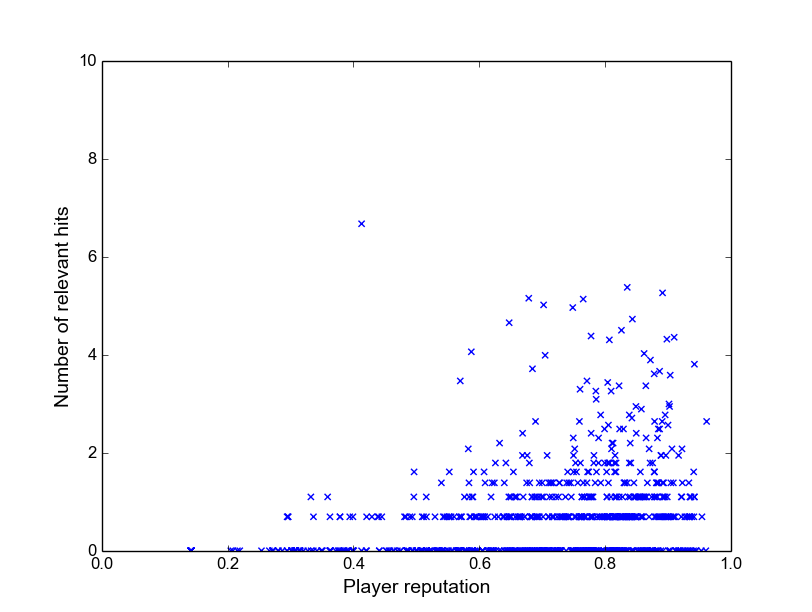
\includegraphics[scale=.4]{filterrepcorr}
\caption{Correlation between the reputation and the number of relevant hits for the players. The horizontal axis displays the reputation of the player in increasing order and the vertical axis shows the number of relevant videos retrieved using a tag entered by the corresponding player.}
\label{filter:fig:repcorr}
\end{figure}

This section outlines the results for the system $S_{F_{prep,k}}$ which takes only the top $k$ tags for each fragment where the ranking is based on the combination of the TF-IDF score and the reputation of the players.
As previously, the value of $k$ was varied from 10 to 100 with an increment of 5.
The best results are achieved for $k=70$ and are displayed in Table \ref{filter:table:map-prec-rec}. As we can see there is a an improvement of $11\%$ with respect to the MAP score compared to the system $SE_{user}$ which indexes all user tags. However, the search performance of  $S_{F_{prep,70}}$ is worse for all three metrics than the system $S_{F_{tfidf,80}}$ which ranks and filters the tags based only on their TF-IDF scores. This means that considering the reputations of the players in combination with the TF-IDF ranking in this case only worsened the matters for the TF-IDF based filtering. This conclusion is further supported by the fact that $SE_{tfidf,80 + catalog}$ outperforms  $SE_{prep,70 + catalog}$ by $5\%$ with respect to the MAP score. 
\paragraph{Discussion} Figure \ref{filter:fig:repcorr} shows the correlation between the reputation of the players and their success in providing tags that resulted in relevant search results. In particular, the horizontal axis shows the reputation for each of the users in increasing order whereas the vertical axis presents the number of relevant video fragments that can be retrieved using tags entered by the corresponding player. As seen, higher reputation does not entail higher success rate. In fact, many of the most  reputable players are among the ones that were the least successful. This means that computing reputation in the manner outlined above may not be the best predictor for the ability of the player to provide topically relevant tags. 
Moreover, considering \cite{DBLP:conf/chi/RobertsonVW09,Jain:2013:GAE:2399187.2399190} our reputation estimation method assigns higher reputation to players which settle on low-effort tags. Consequently, tags favored by this filtering method will tend to be more `obvious'.
Alternative explanation is that there is not sufficient data available to reliably estimate the reputation of the players. Recall that 99\% of the players are registered as anonymous and the only data available for them is a single session of playing \textit{Waisda?}. 

\subsubsection{\textit{\textit{TF-IDF-rank Take Top k}}}

\begin{figure}
\centering
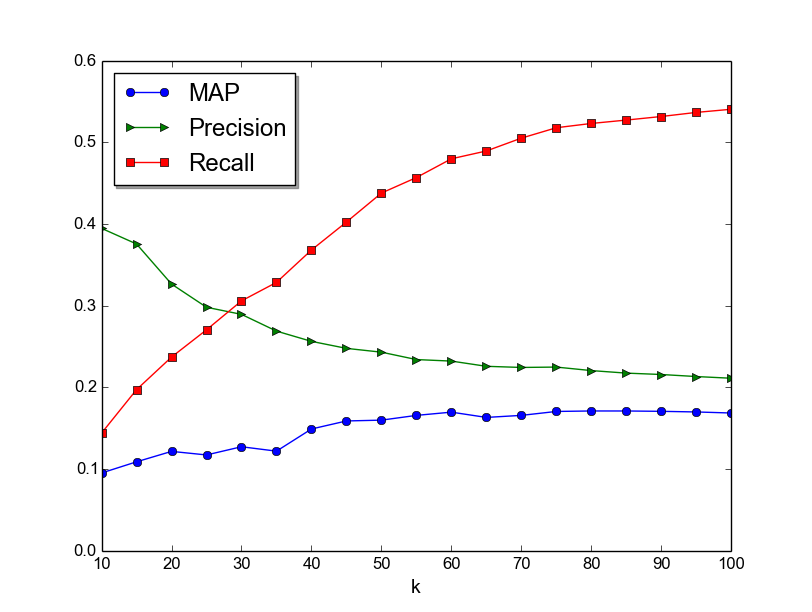
\includegraphics[scale=.4]{tfidfmets}
\caption{Search performance statistics for the systems $SE_{F_{tfidf,k}}$.}
\label{filter:fig:tfidfstats}
\end{figure}

This section outlines the results for the systems $S_{F_{tfidf,k}}$ which consider only the top $k$ tags for each fragment where the ranking is based on the TF-IDF scores of the tags. We vary the value of $k$ from 10 to 100 with increments of 5. Figure \ref{filter:fig:tfidfstats} presents the search performance statistics as the value of $k$ varies. Not surprisingly, as the value of $k$ increases the search precision and the search recall decrease and increase, respectively. Moreover, the MAP score steadily increases until $k$ equals 80, where the maximal value is reached, and then it starts to decrease. As shown in Table \ref{filter:table:map-prec-rec}, the MAP score of $S_{F_{tfidf,80}}$ is $0.171$ which means it significantly outperforms $SE_{user}$, the systems that indexes all user tags. Indeed, the increase in search performance is 31\%. What is more important is that $S_{F_{tfidf,80}}$ slightly outperforms even $SE_{catalog}$, which until now was the best performing one and the system that we are trying to beat. This suggests that TF-IDF score is indeed a good indication of the quality of the tags as topical descriptors and can be used to filter out the non-topical tags. Furthermore, the combination of catalog metadata and TF-IDF filtering proves to be beneficial: $SE_{tfidf,80 + catalog}$ outperforms  $SE_{catalog}$ by $18\%$. The improvement is caused by the fact that the TF-IDF ranked tags increase the search recall of the catalog metadata by factor of $2$; the recall of $SE_{tfidf,80 + catalog}$ is higher than the recall of $SE_{catalog}$ by $107\%$.

\section{Conclusion and Discussion}\label{sec:topicir-filter:con}
In this paper we studied to what extend players enter tags which are valid topical descriptors of the video material. Another aim was to derive insights about players’ tagging practices that are associated with ascribing topical tags. The study was carried out with the focus on topical search.

In Section \ref{sec:topicir-filter:all-tags} we evaluated the search performance of the entire unprocessed collection of the user tags. The general conclusion is that the search performance of the raw, unprocessed, user tags for retrieving videos based on topic leaves much to be desired. While the search recall of the user tags is relatively satisfactory the precision is rather poor. Our analysis showed that a significant portion of the topics are indeed captured by the user tags. However, there are also many user tags that do not pertain to the subject (\textit{semantics}) of the video, but refer to the more \textit{syntactic} aspects such as what is \textit{seen} or \textit{heard}. It is the latter group that is responsible for the false positives and thereby hurting the search precision. Therefore, if user tags are to be used for topical search, a preprocessing step is required that will identify and filter out the non-topical user tags.

The quality of the tags as topical descriptions was addressed in Section \ref{sec:topicir-filter:filtering} where we looked into several ways we can detect and filter out the non-topical user tags. While the different methods that we studied performed with various success, the conclusion is that the game tags can be successfully exploited for topical video search provided there is a filtering process that would reduce or eliminate the effect of the non-topical tags. Our results show that after TF-IDF-based filtering game tags can emulate the retrieval performance of the best performing system that utilizes manually crafted metadata for search. Moreover, combining TF-IDF filtered game tags with the manually crafted metadata  yields an improvement of retrieval performance by $18\%$. The improvement is attributed to the increased retrieval recall stemming from the game tags. An important consequence of this result is that tagging games provide a cost-effective alternative for AV collection owners that do not possess the required manpower to manually annotate their material.

Successfully deploying a GWAP is no small feat. Atracting new players and keeping them engaged over time is vital for success and requires continuous publicising efforts. The experience gained from the \textit{Waisda?} project showed that targeting the fanbase of the TV series being tagged in the game is an effective method of attracting new players. Player’s engagement can be sustained with in-game motivational mechanisms such as leaderboards, and with time-limited contests offering awards for the top performers. Planning and executing such activities is costly, however the cost is independent of the size of the video collection.  The cost of manual annotation, on the other hand, increases linearly with the size of the collection and will eventually outweigh the \textit{Waisda?}-related costs.

What makes video annotation a difficult task is the fact that video is a medium that is extremely rich in meaning. The taggers can get overwhelmed by the complex interplay of objects and events especially in the fast-paced game setting. Our qualitative analysis showed that significant portion of the \textit{Waisda?}
tags refer to more noticeable aspects of the content such as moving objects in the background or in the foreground, or prominent stationary objects. This is hardly surprising, after all these are things that are easy to reach consensus on and ultimately that is the goal of the game from the perspective of the players. We also observed that the tags which are present in the audio and refer to a concept that appears visually are more likely to be topical descriptors. Their presence in both the audio and visual component is an indication that they are denoting salient aspects of the content. Therefore, if the goal of the AV collection owners is collecting topical tags, this insight can be operationalized in the game by instructing the players to tag things that are both on screen and in the audio.

\textit{Waisda?} is a production grade open-source crowd-sourcing tool which is relatively easy to set-up and after the suitable processing the collected tags can be exploited for retrieval. We believe that this is an important step toward making the AV heritage more accessible on the Web and in general making the Web more connected.


\chapter{\textit{Waisda?}:Open-source Video Labelling Game}\label{chap:waisda}

\begin{quotation}
\noindent 
In this chapter we shall describe in more detail the video labelling game \textit{Waisda?} and how it can be exploited as a crowsourcing tool for collecting user-generated tags for video clips. We shall also outline the results and efforts from this thesis that had an impact on the development of \textit{Waisda?}.

This chapter is based on the paper entitled \textit{Waisda?: video labeling game} which was presented at Proceedings of the 21st ACM international conference on Multimedia, held in Barcelona, Spain. The paper is authored by Michiel Hildebrand, Maarten Brinkerink, Riste Gligorov, Martijn Van Steenbergen, Johan Huijkman, and Johan Oomen.
\end{quotation}

\section{Introduction}

In essence, \textit{Waisda?} is a Game With A Purpose (GWAP). GWAPs are a human-based computation technique in which a computational process performs its function by outsourcing certain steps to humans in an entertaining way \cite{Ahn:2006:GP:1155311.1155342,gwap}. The crux of this approach is the realization that humans are better than computers in certain tasks. For example the computers still lack the basic conceptual intelligence or perceptual capabilities required for carrying out the task of labelling random images and videos \cite{Ahn:2006:GP:1155311.1155342}. In fact, the first example of a GWAP, the ESP Game created by Luis von Ahn, labels images on the Web by harnessing the capabilities of the players. The ESP game randomly pairs up two players with the task to describe images. Players don't know who their partner is, nor can
they communicate with each other. The only thing partners have in common is an image they can both see.
When both players provide the same label for an image, they score points and proceed to the next image. The labels entered by both users are associated to the image as metadata. In other words, the consensus among players is a mechanism to ensure the quality and consistency of the labels. The same design principles are applied in \textit{Waisda?} as well. \textit{Waisda?} is a multi-player labelling game where players compete with each other by tagging streaming video. The players score points by entering the same tag as one of the other players within a ten seconds interval. As a result, the video that is tagged in the game is annotated with the matched tags which are anchored to the time points in the video when they were entered.

\textit{Waisda?} was conceived by the Netherlands Institute for Sound and Vision (S\&V) and the VU University Amsterdam in the context of the Dutch project Images for the Future\footnote{\url{http://imagesforthefuture.com/}} and the European research project PrestoPRIME, as an open-source crowdsourcing tool that can be deployed by multimedia collection owners as crowdsourcing initiatives to annotate their collection items. The development of the software was contracted to Q42, a Dutch internet development company\footnote{\url{http://q42.com/}}. The Netherlands Institute for Sound and Vision in cooperation with Dutch broadcasters deployed \textit{Waisda?} in two consecutive pilots featuring historical archive material as well as recent TV episodes from Dutch shows. The first pilot of the game run from May 2009 until January 2010 and produced over $420,000$ user tags. The follow up analyses of the collected tags \cite{Annelies,ecir} and user evaluations suggested potential areas of improvement. Considering the acquired experience and insights, S \& V launched a second pilot of the game\footnote{At the time of writing, the game is deployed online and can be accessed at \url{http://woordentikkertje.manbijthond.nl/}.} which featured several improvements, albeit the basic idea of the temporal tag agreement is preserved. The two pilots together resulted in more than a million tags describing thousands of videos. In fact, the studies described in Chapter \ref{chap:kcap} and \ref{chap:ecir} are based on the data collected in the first and the second pilot, respectively.

The open source version of Waisda? enables maintainers of an online video collection to start their own crowdsourcing initiative for time-based annotations. In particular, we believe that Waisda? is a valuable tool for cultural heritage institutions, as it provides a novel and engaging way for the public to access and interact with the audiovisual material.

In the rest of this chapter we shall describe the gameplay and the user interface of \textit{Waisda?}, explain the software architecture, and give examples of successful deployment of \textit{Waisda?} by third parties. In the final section we outline the results and efforts from this thesis that had an impact on the development of \textit{Waisda?}.
We conclude this section with a list of the awards\footnote{The list of awards is complete up to the time of writing.} given to the \textit{Waisda?} project 
\begin{itemize}
\item \textit{Waisda?} won the \textit{Best Archives on the Web} award in the category \textit{Best Use of Crowdsourcing} in 2010.
\item \textit{Waisda?} won the \textit{EuroITV Competition Grand Challenge} in 2010.
\item \textit{Waisda?} won the \textit{TIMAF European Best Practices} award in 2009
\end{itemize}


\section{Gameplay and User Interface}
The gameplay of Waisda? is straightforward: the player first selects a video from the \textit{Homepage}, plays the \textit{Game} by watching the video and entering tags, and finally studies the results in the \textit{Game recap} to learn what he/she can improve in future games.

\subsection{Homepage}
Figure \ref{homepage} shows the homepage of \textit{Waisda?}, with six videos that the user can choose from. A player starts a game by selecting one of these videos. To give other players the opportunity to join the game, the player first enters the waiting room. In the waiting room the players can study the game
instructions and after 20 seconds the game is automatically started. On the homepage the games that are waiting for players are shown at the bottom right. Players can quickly join a game by selecting one of the entries.
The homepage also contains the basic instructions that prepare the user for the game. To honour the top players, and motivate the other players, the homepage contains a leaderboard that displays the top players of the week. To engage the players with the purpose of the game a notification at the top of the page shows the total number of tags that were entered into the system, and the users contribution to this total. This part of the page also contains the links to register and login. Games can be played without registering, but only for registered players the score is maintained in the player’s profile. To explain the potential of the contributed tags, the page contains a tag cloud with the most popular tags. By selecting a tag the user can navigate the video collection. Finally, the bottom of the page has space reserved for logos and navigation links to additional pages, such as an about page or a page with the terms of use.

\begin{figure}[t!]
\centering
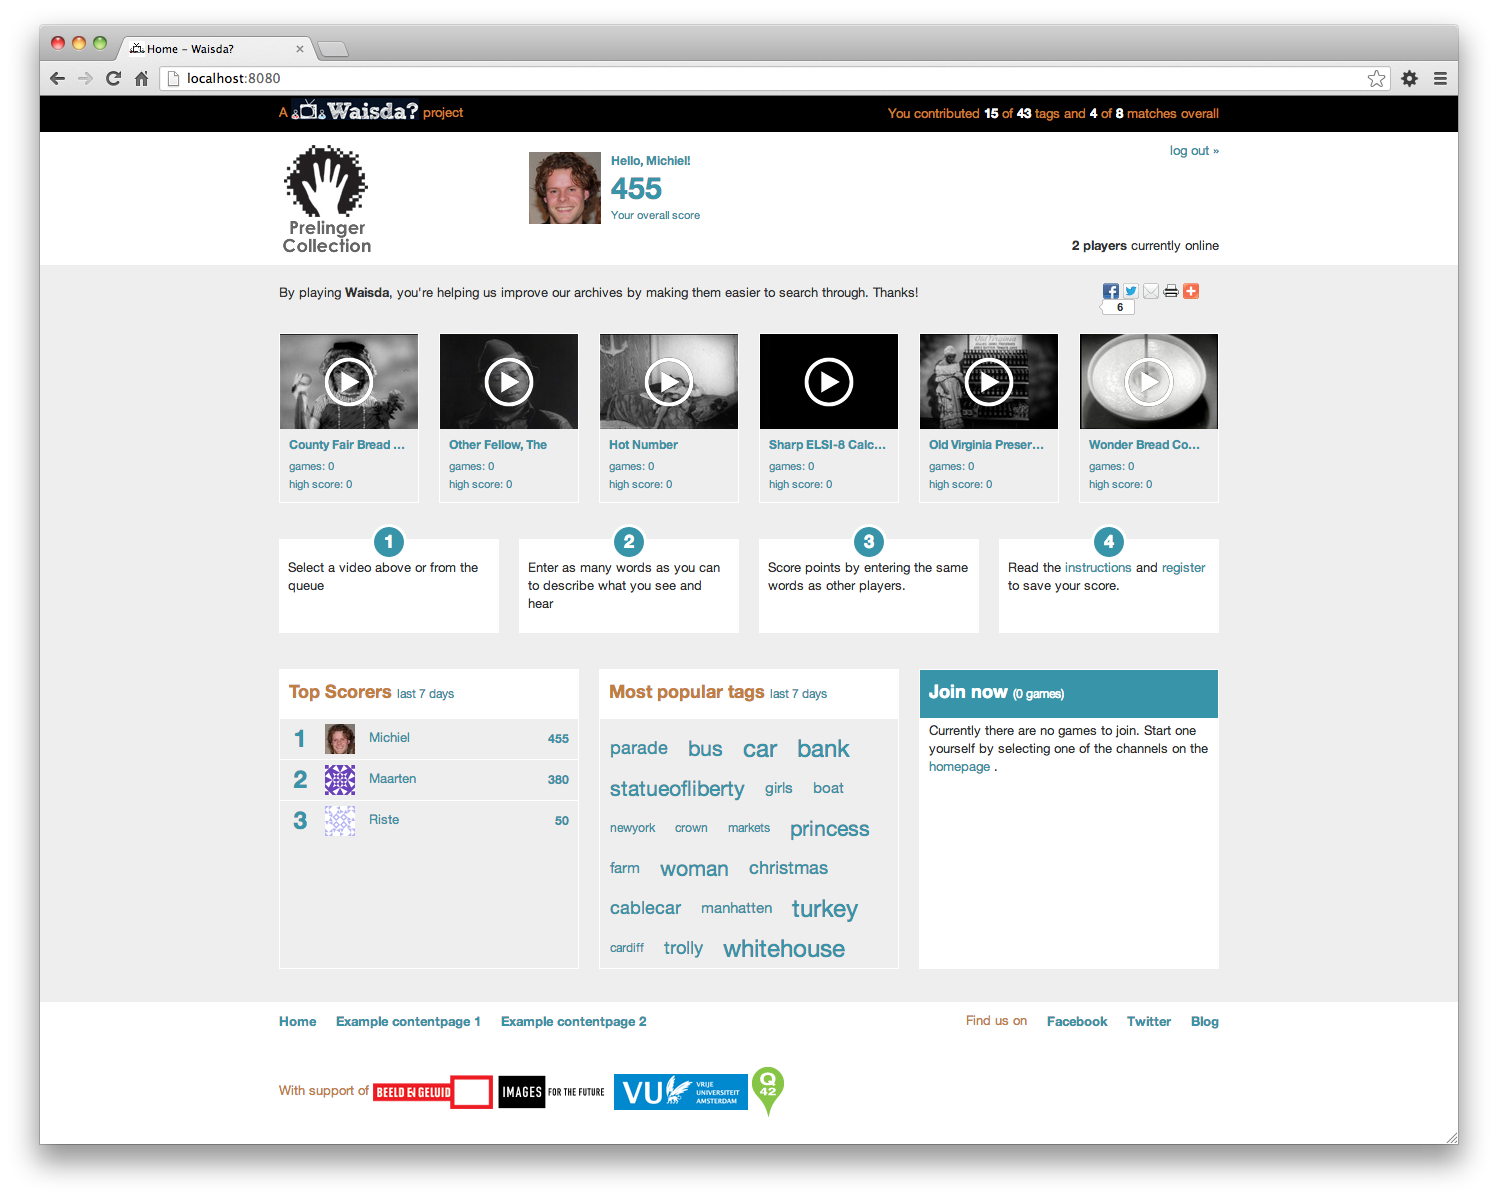
\includegraphics[width=\columnwidth]{figs/homepage} 
\caption{Screenshot of the Waisda? homepage with public domain video clips from the Prelinger Archives.}
\label{homepage}
\end{figure}

\subsection{Game}\label{sec:waisda-game}

Figure \ref{game} shows the game page of \textit{Waisda?}. It contains a video player and below it a text-entry field. When the player enters the game page the video automatically starts playing, the text-entry field receives focus, and the player can start entering tags. The right side of the page contains the score board. It consists of the current score of the player, the current rank and a listing with all tags entered by the player.
The tags are displayed with their score and an icon indicating the type of match and the tag type (person, location etc.).

\textit{Waisda?} uses a scoring mechanism to motivate users to (keep) playing the game, and reward them for entering specific types of tags. The basic scoring mechanism is tag agreement, two players entering the same tag. From the perspective of the video collection tag agreement provides a mechanism to improve the quality, tags that are entered by more than one user are less likely to contain spelling errors and are more likely to provide a trustworthy description of the video. Tags are considered a match if they are syntactically
the same after normalization and entered within a ten second interval of each other. The details of the normalization procedure are explained in the documentation. The matching procedure can be extended by importing tag similarity lists. For example, tags can be matched semantically by importing synonym lists, and specific tags (e.g. Labrador) can be matched with more generic tags (e.g. Dog) by importing word pairs derived from the hierarchical structures of linguistic or domain specific thesauri.

\textit{Waisda?} also contains a mechanism to reward players for entering specific types of tags. For example, when tagging videos in the art domain the names of artists are important. By importing a dictionary with artist names \textit{Waisda?} detects these tag types and rewards the players additional points.

As we can not expect that there are always sufficient users active at the same time, the scoring mechanism of \textit{Waisda?} also motivates users to play alone. In this case a player scores points by matching with the tags that were entered for the same video in previous games. To ensure players not
only tag in the most obvious ways, the scoring mechanism of \textit{Waisda?} also motivates players to \textit{pioneer} new tags. A player enters a pioneer tag when this tag is not entered for this video before, and afterwards it is matched with tags entered by other players (in the same or a later game).

\begin{figure}[t!]
\centering
\includegraphics[width=\columnwidth]{figs/game} 
\caption{Screenshot of the Waisda? game page with public domain video clip from Preligner Archives.}
\label{game}
\end{figure}

\subsection{Game Recap}

When the video ends the user is automatically redirected to the game recap (see Figure \ref{recap}). On this page the user can investigate his/her performance, learn about the details of the scoring mechanism and the behaviour of other players. The game recap consists of two parts. The tag statistics, placed on the left part of the screen,give an overview of the number of tags entered by the player in different categories, including the number of matched tags, pioneer tags and specific types of tags. The tag details, placed on the right part of the screen, are listing of all the tags entered by the player. The listing is similar as the one provided in the game, but includes information about other player in the game, if any, who entered the same tag within a ten seconds interval i.e. a tag match has been achieved.

\begin{figure}[t!]
\centering
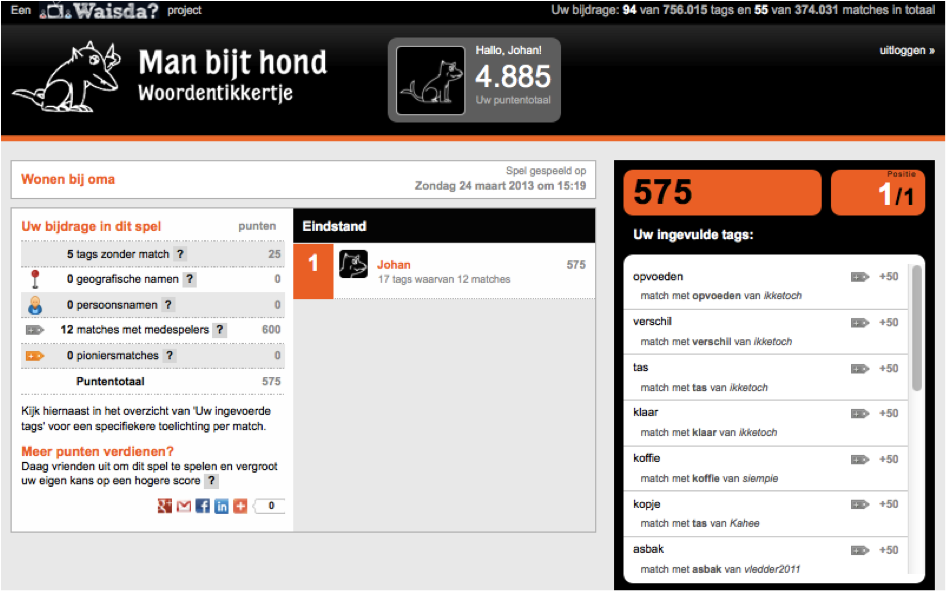
\includegraphics[width=\columnwidth]{figs/recap} 
\caption{Screenshot of the Waisda? \textit{game recap} after a successfully finished game.}
\label{recap}
\end{figure}

\section{Implementation}
\textit{Waisda?} is an open source crowdsourcing tool that has been designed and implemented as a 3-tier web application. The backend application logic is implemented in the Spring Framework\footnote{\url{http://spring.io/}}, which at the time of writing is one of the most widely used open source Java application frameworks. The application is backed by a MySQL\footnote{\url{http://www.mysql.com/}} database which is accessed via the Java Persistence API and Hibernate\footnote{\url{http://hibernate.org/}}. The user interface (UI) is rendered using the Java Server Page (JSP) technology. The UI consists of HTML, JavaScript, and CSS. jQuery and Twitter Bootstrap are used as the JavaScript and CSS libraries. The dynamic
stylesheet language LESS is used to allow easy configuration of the presentation style.

The Waisda? source code and documentation is available from Github \url{http://github.com/beeldengeluid/waisda}. The building, installing and running or the \textit{Waisda?} source code is handled by Maven\footnote{\url{http://maven.apache.org/}} which is a open-source software project management tool developed by the Apache Foundation. The getting started section of the documentation contains instructions to setup a deployment using videos from the Prelinger archive\footnote{\url{http://archive.org/details/prelinger}}.

\subsection{Backend}
After installation the maintainer has to populate the database with videos and optionally with dictionaries and similarity lists. A \textit{video} has a title, description, source URL, key frame URL, duration and video player type. There are currently two types of video players supported: the JWPlayer (HTML5 and Flash), and the NPO player (Silverlight). The latter is used to play content from Dutch public broadcasting associations. Each video in the project specifies which of the two players it would like to use, in combination with the parameters required for the players. To facilitate more robust scoring schemes auxiliary resources like dictionaries and similarity lists can also be used. As long as the data format is valid, the party that deploys the game is free to use any resources it pleases. A \textit{dictionary} is a set of word-type pairs which is used to reward additional points for specific types of tags. Examples are names of celebrities and names of geographical locations. A \textit{similarity list} is a set of word-word pairs which is used to extent the default syntactic tag matching with semantic similarity matching. Examples are synonym pairs or words that are hierarchically related (specific-generic).

\begin{figure}[t]
\centering
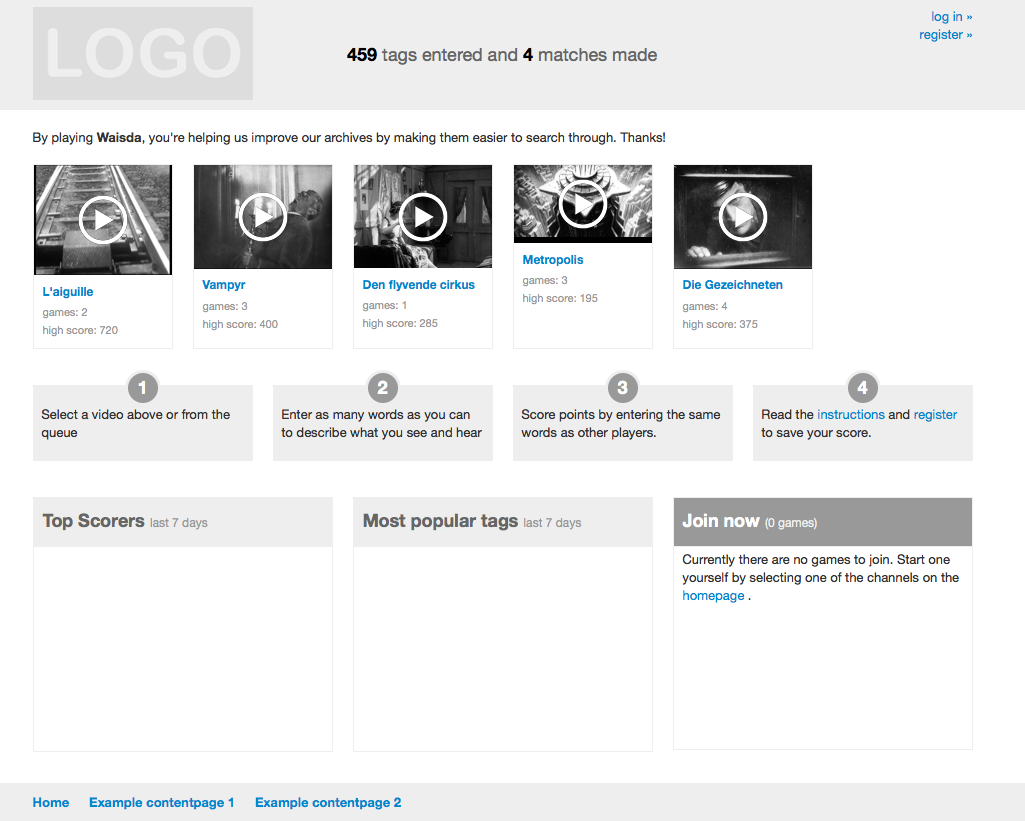
\includegraphics[width=\columnwidth]{figs/waisdastripped} 
\caption{Screenshot of the default user interface of Waisda? stripped of all branding and styling.}
\label{waisdastripped}
\end{figure}

\begin{figure}[t]
\centering
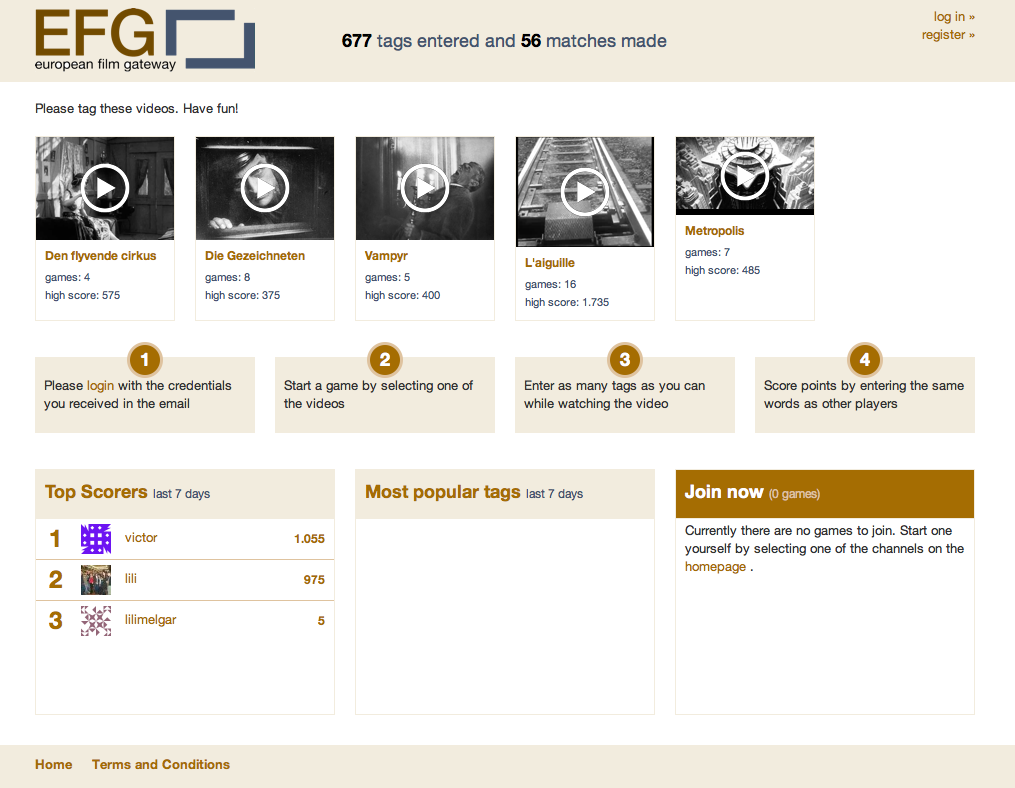
\includegraphics[width=\columnwidth]{figs/waisdaefgtheme} 
\caption{Screenshot of an experimental setup of Waisda? for the European Film Gateway (EFG). It is configured with five videos and the user interface contains a logo and an EFG colour scheme.}
\label{waisdaefgtheme}
\end{figure}

\subsection{Frontend}
The default user interface of \textit{Waisda?} is completely functional. In addition, basic branding and styling can be done by adding a logo and changing the color scheme. These changes can be made with little knowledge of the system and are described in detail in the documentation. The documentation also describes how a maintainer can modify the advanced functionality of the system, such as the videos that are shown on the homepage, how tags are matched and which scores are given. It also describes how new pages can be added or how the page layout can be changed. Making such changes requires more advanced knowledge of HTML, CSS and Java Server Pages. Figure \ref{waisdastripped} shows the basic \textit{Waisda?} interface stripped from all branding and styling whereas Figure \ref{waisdaefgtheme} shows an experimental setup of \textit{Waisda?} styled with the logo and the colour scheme of the European Film Gateway\footnote{\url{http://www.europeanfilmgateway.eu/}}.

\section{\textit{Waisda?} Deployments}
In this section we present several examples of deployments of \textit{Waisda?} in the wild.

\subsection{Europeana}\label{sec:waisda-europeana}
Perhaps the most notable deployment of \textit{Waisda?} is in the context of the Europeana project\footnote{\url{http://www.europeana.eu/}}. Europeana is an internet portal that provides multi-lingual access to millions of books, paintings, films, museum objects and archival records that have been digitised throughout Europe. More than 2,000 institutions across Europe have contributed to Europeana. These range from major international names like the Rijksmuseum in Amsterdam\footnote{\url{https://www.rijksmuseum.nl/}}, the British Library\footnote{\url{http://www.bl.uk/}} and the Louvre\footnote{\url{http://www.louvre.fr/}} to regional archives and local museums from every member of the European Union. Together, their assembled collections let users explore Europe's cultural and scientific heritage from prehistory to the modern day. The Europeana project incorporates the tools, solutions, and preservation practices developed in the PrestoPRIME project\footnote{As mentioned already \textit{Waisda?} is one of the deliverables of the PrestoPRIME project.The publicly available deliverable report can be found at \cite{prestoprime-report}.}. One of the main contributions of the PrestoPRIME project incorporated in Europeana is an OAIS-compliant preservation framework capable of supporting the whole range of digital preservation operations in the long term. \textit{Waisda?} is integrated in the workflows and processes included in this framework that deal with user-generated annotations for videos. In order to provide programmable interaction between \textit{Waisda?} and the other systems in the framework, in the scope of this thesis, an extension module of \textit{Waisda?} was developed. The module consists of a number of web services that enable \textit{adding}/\textit{updating} videos that are to be tagged in the game and \textit{extracting} the collected tags in a light-weight and highly-portable textual format. More details on this can be found in section \ref{chap:waisda:thesis-soft}.

\subsection{Spotvogel}
Another application of \textit{Waisda?} is the so-called \textit{Spotvogel}\footnote{\url{http://spotvogel.vroegevogels.vara.nl/}} which translates to \textit{mocking bird} from Dutch. \textit{Spotvogel} was deployed by the Dutch broadcaster VARA\footnote{\url{http://www.vara.nl/}} and the S\&V institute with the aim of collecting user tags for the footage from the Dutch television program \textit{Vroege Vogels}\footnote{\url{http://spotvogel.vroegevogels.vara.nl/}} (Early Birds in Dutch) which is about wildlife. The goal of the game from the perspective of the players is to identify and tag occurrences of birds and other wildlife in the footage. The players are encouraged to be as specific as possible when identifying the species of the wildlife they are tagging. For example, a tag such as ``long-eared bat" yields more points than the more generic tag ``bat". This is achieved by using controlled vocabulary which contains various names of bird species. Whenever a player enters a recognizable bird species name she or he is awarded extra points. This positive reinforcement is meant to stimulate and reinforce this kind of tagging behaviour in players. The broadcaster VARA counts on the collected tags to increase the accessibility and the searchability of their archive. 

\subsection{European Film Gateway Experiment}
This example differs from the previous ones in the fact that in this case \textit{Waisda?} was used as a tool to carry out an experiment. The experiment was designed and performed by Liliana Melgar Estrada during her stay at the VU Universty Amsterdam and resulting paper \cite{liliana} was accepted for publication in the Journal of the Association for Information Science and Technology. The experiment focuses on studying the differences between how film experts and novices describe (tag) fiction films. As a source material, five videos (fiction clips) from the European Film Gateway were chosen. The act of annotating the videos by the experts and novices was carried out using a customised \textit{Waisda?} installation set up specifically for this purpose. What is worth mentioning is that the customisation capabilities available in \textit{Waisda?} out of the box were sufficient to satisfy the requirements put forward by the experimental design.

\section{Thesis Contributions} 
In the final section we outline the contributions of this thesis for the development of \textit{Waisda?} which fall into two areas \textit{software development} and \textit{game design}.
\subsection{Software Development}\label{chap:waisda:thesis-soft}

\begin{figure}[t!]
\centering
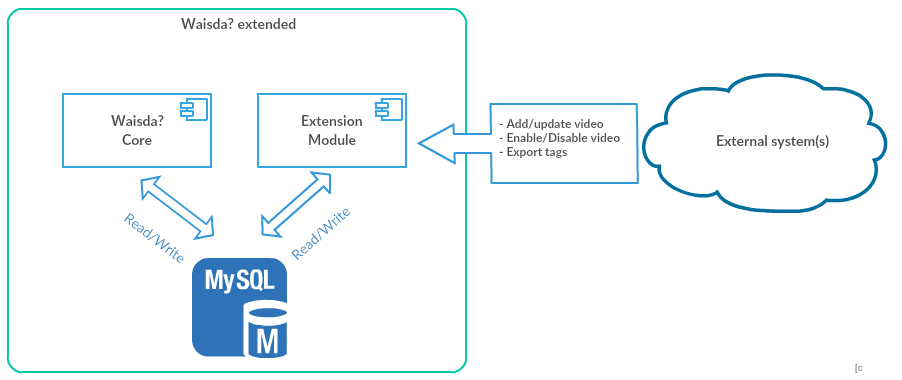
\includegraphics[width=\columnwidth]{waisda-diagram} 
\caption{\textit{Waisda?} architectural diagram: interaction among \textit{Waisda?} core, the extension module, and external systems.}
\label{waisda-diagram}
\end{figure}

As mentioned in Section \ref{sec:waisda-europeana}, \textit{Waisda?} has been integrated into the framework that fuels the Europeana internet portal. In order to provide programmable interaction between \textit{Waisda?} and the other systems in the framework, we developed an extension module of \textit{Waisda?}. The module has been developed in Java programming language and uses the same technology stack as the Waisda? core. In particular, the application logic is implemented in the open-source Spring framework and the access to the database is facilitated by the Java Persistence API and Hibernate. Figure \ref{waisda-diagram} shows the architecture overview and the flow of data among the \textit{Waisda?} core, the module, and external systems. The \textit{Waisda?} core and the module communicate through shared database. Both components read and write data to the same underlying MySQL database. In literature, this is referred to as \textit{shared database} enterprise integration pattern \cite{Hohpe:2003:EIP:940308}. All direct interaction from the outside world with the database goes through the module which acts as a gateway. External systems read and write data using the services defined by the module. External systems and the module exchange messages encoded in the lightweight highly-portable data-interchange JSON\footnote{\url{http://www.json.org/}} format. This allows for high-level of decoupling and interoperability between \textit{Waisda?} and external systems which can be implemented in any programming language without any knowledge about the underlaying technical details of \textit{Waisda?}.

The module consists of the following services:

\begin{figure}
\centering
\begin{lstlisting}[language=json,firstnumber=1]
{
	"title": "American flamingo",
	"playerType": "JW",
	"sourceUrl": "http://goo.gl/Jw577N",
	"fragmentID": 1,
	"imageUrl":"https://goo.gl/NmBq47",
	"enabled": true,
	"startTime": 0,
	"duration": 740000
}
\end{lstlisting}
\caption{JSON data request payload for the \textit{video submission/update} web service. The data payload consists of metadata for the video that is to be submitted or updated.}
\label{chap:waisda:add-update-json}
\end{figure}


\begin{figure}
\centering
\begin{lstlisting}[language=json,firstnumber=1]
{
	"fragmentID": 1,
	"enabled": true,
]
\end{lstlisting}
\caption{JSON data request payload for the \textit{enable videos for tagging} web service. The data payload consists of an object which contains a \textit{fragmentId} which identifies the video to be acted on and a boolean \textit{enabled} flag.}
\label{chap:waisda:enable-json}
\end{figure}

\begin{figure}
\centering
\begin{lstlisting}[language=json,firstnumber=1]
{
	"fragmentID": 1,
	"timestamp": 2017-03-13T19:55:07+00:00,
}
\end{lstlisting}
\caption{JSON data request payload for the \textit{export tags for video} web service. The data payload consists of an object which contain a \textit{fragmentId} which identifies the video and an optional timestamp.}
\label{chap:waisda:export-json}
\end{figure}

\begin{figure}
\centering
\begin{lstlisting}[language=json,firstnumber=1]
[{
	"tag": "flamingos",
	"videoTime": 3000,
	"tag_id": 1
	"player_id": 42
},
	.
	.
	.
{
	"tag": "beach",
	"videoTime": 45000,
	"tag_id": 28
	"player_id": 1014
}]
\end{lstlisting}
\caption{JSON data response payload for the \textit{export tags for video} web service. The data payload consists of an array of tags entered after the specified timestamp.}
\label{chap:waisda:export-json-result}
\end{figure}

\begin{itemize}
\item \textit{Video submission service}. Using this service external systems can add new videos for tagging in \textit{Waisda?}. Figure \ref{chap:waisda:add-update-json} shows the format of the JSON message that is expected by this service. As seen, the external system needs to provide basic video metadata, such as the title, duration, URL from which the video can be streamed, fragment ID used to identify the video subsequently, video player type, etc. It should be noted that the video itself is not uploaded to \textit{Waisda?}, instead the video is streamed from the provided URL. When calling this service it is assumed that no other video with the provided fragment ID exists already. Failing to comply with this requirement will result in an error.

\item \textit{Video update service}. Using this service the metadata of videos already within Waisda? can be changed. This service accepts the same type of JSON message as the submission service above. It is assumed that video with the specified fragment ID exists already. If this condition is not satisfied, an error will be raised.

\item \textit{Video enable/disable service}. Using this service external systems can \textit{enable/disable} a video for tagging in Waisda?. Figure \ref{chap:waisda:enable-json} shows the format of the JSON message that is expected by the service. The fragment ID of an already existing video in the system needs to be provided along with the flag that determines whether the video should be enabled or disabled.

\item \textit{Video tags export service}. Using this service all tags for a specific video can be exported in JSON format. The data being exported can be limited to tag entries after a certain timestamp, enabling efficient sync mechanisms. Figure \ref{chap:waisda:export-json} shows the format of the JSON message expected by this service. External systems need to provide a fragment ID of an existing video in the system and an optional time-stamp. If a time-stamp is provided, all tags for the video entered after the specified time-stamp will be returned. Otherwise, all tags for the video will be returned. Caller external systems are advised to provide a time-stamp to reduce the number of tags returned. This is merely an optimization step. Figure \ref{chap:waisda:export-json-result} shows the format of the result returned by this service.
\end{itemize}

It should be noted that, while initially developed for the Europeana environment, these services are not bound to it in any way and can be seamlessly integrated in any system or workflow. The only requirement is that the external systems ought to honor the contract defined by the services when calling them. The services provide a basic set of operations that can be used to implement more complex real-life scenarios involving \textit{Waisda?} as a crowdsourcing tool for collecting video annotations.
\subsection{Game Design}\label{chap:waisda:game-design}
The development of \textit{Waisda?} proceeded in two iterations. After the first pilot was launched the follow up analyses of the collected tags \cite{Annelies,ecir} and user evaluations suggested potential areas of improvement. The suggestions were incorporated into the game design and the second, which is also the current, version of \textit{Waisda?} was rolled out.

One of the follow up studies \cite{ecir} was carried out in the context of this thesis and it is covered in detail in Chapter \ref{chap:ecir}. In this study we noticed limitations or the game tags collected in the first pilot. One limitation is the low number of specific type of tags in the \textit{who} and \textit{where} facets i.e. \textit{persons} and \textit{locations}. We showed that by matching the tags to controlled vocabularies we can derive the type of the tags (person, location, organization, etc.). We suggested a modification in the scoring mechanism where the players are awarded extra points for entering specific types of tags e.g. persons or locations (see Section \ref{sec:waisda-game} for details). This positive reinforcement is meant to stimulate and reinforce this kind of tagging behaviour in players. Another limitation of the first version of \textit{Waisda?} was the way the tags entered by different players were compared, which was basically a case-insensitive string comparison. We suggested extension of the matching mechanism where synonyms, hyponyms, and hyperonyms would also be considered a match (see Section \ref{sec:waisda-game} for details). Both suggestions were approved and are now part of \textit{Waisda?}.

The other follow up study \cite{Annelies} was conducted by Annelies van Ees in the context of her master thesis project. The aim of the study was to determine factors that motivate people to play a video tagging game such as \textit{Waisda?}. The conclusion of the study was that players are more inclined to play when videos are shorter and more feedback is provided. The feedback in this case was in the form or game recap once the game is finished. Based on these findings the second pilot included short videos
%\footnote{The average duration of the videos in the collection was $3.3$ minutes and the median was $3.6$ minutes.} 
and also featured a game recap screen (see Figure \ref{recap} for details).

\section{Conclusion}
In this chapter we described Waisda which is an open-source crowdsourcing tool that can be deployed by audio-visual collection owners to annotate their collection items. We outlined the main technological aspects of the game, the gameplay, and the key user interface features. At the time of writing, the latest release of Waisda is a mature, production-grade, customizable \textit{game with a purpose}, with a diverse usage. Many aspects of the game can be customized, such as the user interface and tag matching mechanisms, in order to fit various application scenarios. 

As part of the research described in this thesis, an extension module to \textit{Waisda?} was developed which enables seamless integration of the game in broader audio-visual workflows. The module features a set of high-level services which hide the underlying technological complexity  and provide communication in the light-weight and highly-portable JSON textual format. The services offer support for the basic \textit{add}, \textit{update}, \textit{read}, and \textit{enable/disable} operations which serve as a basis on which more complex integration scenarios can be built. Having said that, and considering the results from Chapters \ref{chap:ecir} and \ref{chap:topicir-filter}, \textit{Waisda?} is valuable tool at the disposal of the audio-visual collection owners which provides cost-effective way of obtaining community-centric video annotations.


\chapter{Conclusions and Discussion}\label{chap:conclusion}
\begin{quotation}
\noindent 
In this chapter we revisit the research questions outlined in Chap. \ref{chap:intro} and state the conclusions that follow from the research work presented in this thesis. We conclude with a final discussion and indicate possible research directions to extend or compliment the results described in the thesis.  
\end{quotation}

As audio-visual archives become accessible to the wider internet audience, successful retrieval of archive items is an increasingly challenging task. One of the most important reason for this is the lack of adequate annotations. Users cannot find what they are looking for because annotations are either not
present or too expert-centric. Video tagging games are an attempt to alleviate this problem. Engaging the internet community to tag the videos addresses the issue of scarcity of annotations and yields tags that are community-centric. The focus of this thesis is on the role of game tags in audio-visual archives and their added value for video retrieval. In the typical audio-visual archive ecosystem the game tags will coexist with professionally curated annotations. To understand what do game tags bring to the table as opposed to the catalogers' annotations we studied the differences between them along two dimensions. The first dimension is the \textit{terminology}: we performed a quantitative study to estimate the \textit{terminological gap} between taggers and the catalogers. The second dimension is the \textit{descriptive scope} i.e. which aspects of the video content are described and at what level of abstraction and granularity. We carried out a qualitative study in which we analysed the descriptive scope of the game tags. Making the videos more accessible to the wider internet audience is one of the main objectives of the game tags. To evaluate the efficiency of the game tags for video retrieval we designed Cranfield-style experiments for two prominent scenarios that arise in practice: \textit{visual} and \textit{topical} search. Moreover we performed a qualitative analysis of samples of search results to establish the reasons that usually lead to true and false positives in both scenarios. The fast pace of \textit{Waisda?} usually results in players contributing mainly non-topical tags. To combat this effect in the visual search scenario, we characterized the quality of user tags as topical annotations and identified several tag features (filters) that serve as indicators whether game tags are useful for retrieval. The success of each of the filters was evaluated in Cranfield-style experiment.

The main contributions of the thesis are:
\begin{itemize}
\item A method to analyze quantitatively the overlap between user and professional terminology exploited in video annotation.
\item Qualitative analysis of the aspects of the video content which are described by the game tags i.e. \textit{what do game tags describe in a video and how}.
%\item A method of qualitative analysis of samples of user tags to establish the facets---\textit{who}, \textit{what}, \textit{where}, and \textit{when}--- of videos typically described by users and the level of specificity---\textit{abstract}, \textit{generic}, and \textit{specific}---of tags.
\item A method to design a dataset ---including fragments, queries, and relevance judgements --- for evaluating the added value of user tags for \textit{visual} and \textit{topical} video search.
\item Two evaluation datasets ---one for visual and one for topical search --- which contain fragments, user tags from \textit{Waisda?} collection, queries, and relevance judgements.
\item Quantitative evaluation of the added value of the game tags in terms of \textit{visual} and \textit{topical} video search.

\item A method for qualitative analysis/classification of the search results in the context of visual search. The aim of the analysis was to discover the types of tags that are generally responsible for false positives.

\item Qualitative analysis of the search results in the context of topical search. The aim of the analysis was to discover tagging practices that generally produce relevant topical tags.

\item Evaluation of tag-related measures for accessing the quality of the game tags as topical descriptors in the context of topical video search.

\item Development of extension module for \textit{Waisda?} which enables integration of the game in AV collection workflows. The module is part of the latest release of \textit{Waisda?} which is available online\footnote{The Waisda? source code and documentation is available from Github \url{http://github.com/beeldengeluid/waisda}}.
\end{itemize}

In this chapter we consider again the research questions stated in Chapter \ref{chap:intro} outlining the methods and results. The last section features discussion and directions for future research.

\section{Research Questions Revisited}
\subsection{What is the relationship between the game tags and professional annotations in terms of vocabulary and what they describe?}
In the typical audio-visual archive ecosystem the game tags coexist with professionally curated annotations.
Successful integration of the game tags into the AV collections' workflows requires a better understanding of the characteristics of the tags compared to the professional annotations. To this end, in Chapter \ref{chap:kcap}, we performed a quantitative and a qualitative study of the game tags in which we compared them to the professional annotations along two dimensions: (i) the vocabulary used i.e. the \textit{terminological gap} and (ii) the aspects of the video content that are described.

\subsubsection{Studying the Terminological Gap}
In order to study the terminological gap we devised and carried out a quantitative analysis of the game tags. 
Presently, \textit{Waisda?} has no built-in mechanisms that control the quality of the language used by the taggers. Therefore, the first goal of the analysis was to determine the fraction of the game tags that are meaningful words. For this purpose we exploited two vast background knowledge sources --- the general lexicon of the Dutch language Corneto and the Google search engine --- as semantic filters; whenever a tag is present in either of these two sources we take it as a signal that the tag is a meaningful word. Additionally, Corneto encodes part-of-speech information about the words which we exploited to quantify the types of words generally used by the taggers. Corneto also provides information about the various senses of the words which was used to detect polysemy. The results from the analysis showed that the majority of the game tags are meaningful words in themselves. This analysis also reaffirmed some of the inherent limitations of the user tags compared to the controlled vocabularies; namely, subjectivity and ambiguity of the language. Using the part-of-speech information we detected that the majority of the tags found in Cornetto are nouns and verbs. This means that people generally focus on objects and actions when tagging the videos. Small fraction of the game tags found in Cornetto, around $15\%$, are adjectives. Generally these are subjective descriptive words, for example the most common adjective among the tags is \textit{lekker} (\textit{nice} in Dutch).

Finally, to check whether there is a terminological gap between the game tags and professional annotations we matched all game tags to the domain thesaurus GTAA. GTAA is the sole vocabulary that is employed by the catalogers when annotating the same videos that are tagged in the game. We observed that only a small fraction of the unique game tags can be found in GTAA, around $8\%$. This showed that there is indeed a terminological gap in the way the gamers and catalogers describe the videos.

\subsubsection{What do the tags describe?}

To get a better understanding of what aspects of the video content are described by the game tags we carried out a manual classification of a sample of game tags. We used a classification schema that combines the Pahofsky-Shatford model and a classification framework built by Hollink at al \cite{laurapaper}. The results of the tag classification demonstrated that the game tags predominantly describe objects using generic language and rarely refer to topics of a scene or the entire video. This is in sharp contrast with the professional annotations which exclusively target the topic(s) of the entire video and (less frequently) of particular scenes. The general conclusion is that game tags and the professional annotations are complementary both in terms of the terminology and in terms of what aspects of the video content they describe. This makes the game tags a valuable asset for at least the following two reasons. First, they provide a more online community-centric view of the content which will undoubtedly improve the access for the wider internet audience. Second, game tags are fine-grained annotations that target scenes, events, and objects within scenes. At this level of granularity they can facilitate tasks like \textit{event detection}, \textit{instance search} etc. Moreover, this level of granularity generally is unattainable for the professional annotations due to the enormous effort and time required. Game tags can step in and fill the void.
\subsection{Can we improve video retrieval with the help of user-generated data?}\label{conclusion:search}
Video fragment retrieval is widely recognized as an application scenario of particular business importance in the AV archival world. We evaluated the effectiveness of the game tags for two retrieval tasks: (i) \textit{visual search}, retrieval of fragments that feature visual appearances of the concept of interest and (ii) \textit{topical search}, retrieval of fragments that are about a given topic.
\subsubsection{Game tags for visual search}
When evaluating the effectiveness of game tags for visual search in Chapter \ref{chap:ecir}, we were mainly interested in two research questions. First, can game tags on their own or in combination with other existing types of metadata improve search? And second, does using only verified (consensus) tags give better search performance than using all game tags? In addressing these questions we used the quantitative system evaluation methodology. To this end, we created an evaluation dataset which consists of (i) a set of video fragments which were tagged in \textit{Waisda?}, (ii) a set of queries derived from real-life query logs, and (iii) relevance judgements. The relevance judgements were collected in a online user experiment wherein participants given a video fragment judged its relevance w.r.t the queries. The participants were instructed to judge a fragment to be relevant for a query if the concept denoted by the query visually appears in the fragment. We then created a number of search systems, ran them against the evaluation dataset and computed retrieval performance measures to assess their search effectiveness. The systems were carefully designed so that the collected evidence is sufficient to answer the research questions.

The results demonstrated that search based solely on game tags significantly outperforms search based on other types of metadata alone. In particular, game tags outperformed the in-house catalog tags and closed captions by $69\%$ and $39\%$, respectively. Moreover, combining the game tags with the other metadata types proved to be beneficial for search. In fact, the search engine that exploited all available metadata performed best, to large part due to the contribution of the game tags --- the observed performance improvement was $33\%$.

Considering only verified tags resulted in worse search performance than considering all game tags. In fact, all game tags outperformed the verified tags by $53\%$. This was mainly caused by the fact that search based on all game tags yields more relevant results and resulted in significantly higher recall. It seems the tag verification criterion is too conservative in a sense that it filters out tags that are in fact useful for search.

In Chapter \ref{chap:ecir} we established that game tags usually describe events and objects within scenes so it is not surprising that they excel at visual search. We also established that there is a difference in the focus and the scope of the game tags compared to the professional annotations; game tags being more fine-grained and professional annotations being more coarse-grained referring to the entire video and describing the prevalent topics. The in-house catalogue tags fit the latter profile: they are scarce and cover the topics of the video. This being said, quite predictably they fall short compared to the game tags when it comes to visual search. The closed-captions, on the other hand, are similar to the game tags in terms of focus and scope. Yet, game tags outperform them. This can be explained by the fact that closed-captions only cover the audio portion of the video and there are some aspects that have only visual representation. However, in order for the game tags to be able to compete with closed-captions there should be a \textit{sufficient} number of them assigned to the videos. What is a sufficient number of tags for a video is very hard to tell but in principle the more tags the better. And with time as more tags are added their search performance is improving and tables are turning in their favour. This was demonstrated in Sect. \ref{ecir:over-time-results}.

The overall conclusion is that game tags are well-suited for retrieving fragments that visually depict given object of interest. This property of the game tags makes them particularly appealing for business use-cases such as discovering/selling stock footage. 

\subsubsection{Game tags for topical search}
In Chapter \ref{chap:topicir-filter} we studied the added value of game tags for topical search. To this end, we used once again the quantitative system evaluation methodology which entails creation of evaluation dataset. When creating the dataset, we reused the same set of queries from the visual search study from Chapter \ref{chap:ecir}. The process of deriving the relevance judgements was automatised by exploiting the in-house catalog tags as the gold standard w.r.t. what topics are covered in the fragments. This allowed us to consider much larger set of fragments for the study since we were no longer dependent on human judges. 

The collected retrieval performance metrics showed that when it comes to topical search the game tags leave much to be desired. While the retrieval recall of the game tags is relatively satisfactory the precision is rather poor. So poor that it outweighs the good recall. The results were even worse for the verified tags. This was rather surprising since the initial expectations were that the consensus among the players reached on verified tags would result in tags that trustworthily describe the prominent aspects of the videos. Our hypothesis was that the tags referring to objects that are visually depicted in the videos are the leading reason for the poor retrieval performance. To test this hypothesis we performed a manual classification of samples of true positives and false positives retrieved using the game tags. The samples were classified w.r.t. to the content component they refer to --- \textit{audio}, \textit{visual}, or \textit{both} --- and using the tag classification schema developed in Chapter \ref{chap:kcap}. The results from the classification confirmed the hypothesis. The majority of the false positives, about $67\%$, were caused by tags referring to concepts that are only visually depicted. Moreover, most of these cases refer to general tags describing objects  appearing in the foreground and the background of the scenery. What is more important, our analysis showed that a significant portion of the topics are indeed captured by the game tags. However, there are
also many user tags that do not pertain to the subject (\textit{semantics}) of the video, but refer to the more \textit{syntactic} aspects such as what is \textit{seen} or \textit{heard}. It is the latter group that is responsible for the false positives and thereby hurting the search precision. Therefore, if user tags are to be used for topical search, a preprocessing step is required that will identify and filter out the non-topical user tags.

\subsubsection{Game tags for retrieval: Folksonomic flaw}\label{conclusion:folsonomy-flaw}
One of the main drawbacks of the user-generated tags compared to the controlled vocabularies is that tags are inherently imprecise, the so-called \textit{folksonomic flaw} \cite{Mathes04folksonomies,citeulike:468899}. The players of \textit{Waisda?} are unconstrained when entering tags and this can lead to several limitations. There is no explicit meaning assigned to the tags which can result in \textit{ambiguity}. For example, the tag \textit{ant} may refer to the eusocial insect of the family Formicidae. However, it may also refer to the relatively well-known software \textit{Apache Ant}\footnote{\url{http://ant.apache.org/}} (usually abbreviated to \textit{ant}). It may even be an acronym for ``Actor Network Theory". Without explicit disambiguation there is no way to tell the intended meaning. Another limitation of game tags stems from the presence of \textit{synonyms} in natural languages. For example, both the tags \textit{mac} and \textit{macintosh} can be used to denote Apple Macintosh computer. If the searcher searches for \textit{mac} but only \textit{macintosh} is present in the system the search will be unsuccessful. Yet another limitation is imposed by the general level of \textit{tag literacy}. Plural and singular forms, conjugated words and compound words may be used, as well as specialised tags and ``nonsense" tags designed as unique markers that are shared between a group of friends or co-workers. These limitations are not exclusive to game tags. The other metadata types suffer from them as well, albeit to a lesser extent. Closed-captions and in-house catalog tags can be ambiguous and have issues with synonyms as well. The literacy is a less of a concern for them given their more controlled nature. 

In the search studies described in Chapter \ref{chap:ecir} and \ref{chap:topicir-filter} we did not use any special mechanisms to combat the tag limitations outlined above. We did use stemming which is a standard technique to deal with word inflexions by reducing the inflected words to their root(stem). Tag literacy was not an issue in our search studies as the queries were all standard words and the word inflexions were taken care of by stemming. In other words, the effect of low literacy tags, was not triggered by the queries in our query set. Ambiguity was also not an issue since the majority of the queries in our query set are not polysemic. And even when there is more than one meaning assigned to the queries usually the difference among them is nuanced so they can effectively be used interchangeably. Synonymy can be addressed by query expansion where the synonyms are added to the query and searched for as well. It will be interesting to extend the studies from Chapter \ref{chap:ecir} and \ref{chap:topicir-filter} to deal with synonyms in future work.

\subsection{Can the quality of user-generated tags for videos be evaluated and improved?}
In Chapter \ref{chap:topicir-filter} we demonstrated that game tags are are not well suited for retrieving video fragments based on topic. This is mainly caused by the overwhelming presence of game tags which are not valid topical descriptors. In the second half of Chapter \ref{chap:topicir-filter} we evaluated the quality of the game tags as topical descriptors with the intention to detect and filter out the ones that are not referring to topics. We explored several methods for predicting the tag quality --- TF-IDF-based filtering, player reputation-based filtering, and topic models to name a few. The success of each method was judged against the evaluation dataset developed in the topical search study.

While the different methods that we studied performed with various success, the conclusion is that the
game tags can be successfully exploited for topical video search provided there is a filtering process that would reduce or eliminate the effect of the non-topical tags. Our results show that after TF-IDF-based filtering game tags can emulate the retrieval performance of the best performing system that utilizes manually crafted metadata for search. Moreover, combining TF-IDF filtered game tags with the manually crafted metadata yields an improvement of retrieval performance by $18\%$. The improvement is attributed to the increased retrieval recall stemming from the game tags. An important consequence of this result is that tagging games provide a cost-effective alternative for AV collection owners that do not possess the required manpower to manually annotate their material.

\section{Discussion and Further Research}
In this thesis we investigated the added value of the tags collected with the video-labelling game \textit{Waisda?} for video fragment retrieval. The general conclusion is that the game tags improve retrieval and on average perform better compared to the manually-crafted metadata and closed captions. This statement comes with three caveats. First, in our setting the \textit{taggers} and the \textit{searchers} originate from the same community which entails significant terminological overlap between the \textit{keywords} used for search and the tags ascribed to the videos. We believe this to be the main contributing factor for the success of the game tags for search in the context of our study. And while it may look like a limitation at first, in practice it is not. The terminology employed when tagging is general enough to cater to the needs of all but the expert searchers which may use more specialized (specific) terms when searching. Second, in this work we considered only \textit{keyword-based search} thus the said improvement in retrieval is limited to this modality. At the time of writing, other search modalities such as \textit{content-based video retrieval} \cite{veltkamp2013state} are gaining more attention, however keyword-based search is still the most prominent one, especially on the Web, and is likely to remain so in future. Third, in this work we focussed on single domain (genre), non-fictional TV Comedy. Naturally, the obtained results are bound to this domain. However, the qualitative analysis of the tags revealed that they are usually general concepts describing visual objects and as such are not so tightly coupled with the genre of the video content they are describing. Our expectation is that the game tags will perform well for most of the non-fictional TV genres which appeal to a wider audience. It remains to be seen whether this will be the case for the fictional genres where more symbolism and abstract expressions can be expected. We hypothesise that without properly instructing the taggers or targeting a niche sub-community of experts the outcome will be less satisfactory.

\subsection{The Bigger Picture}
In the recent years there were advancements in many fields that are related to the scope of the work presented in this thesis. Following is a non-exhaustive list of the most relevant ones.

\subsubsection{Computer Vision} Thanks to the advancements made in the area of deep learning \cite{Bengio:2013:RLR:2498740.2498889,Arel:2010:RFD:1921914.1921920,Schmidhuber:deep-learning} the field of computer vision witnessed important breakthroughs in the recent years. Using vast number of high-resolution example images, the deep convolutional neural networks can be trained to classify and label scenes and objects depicted in new unseen images \cite{NIPS2012_4824,10.1109/TPAMI.2012.231}. An excellent example of this idea put into practice is the Microsoft's Project Adam \cite{project-adam}. The Adam computer vision system is hailed to be advanced enough to tell the difference, for example, between a picture of a Pembroke and a Cardigan Corgi (dog breeds), a task that is quite difficult even for a person. The Adam system is fuelled by a deep convolutional neural network which has been trained with over 14 million images split up into 22,000 categories drawn from the ImageNet database\footnote{\url{http://www.image-net.org/}}. Another computer vision task that has benefited greatly from deep learning is face recognition. The Facebook's DeepFace system is able to tell whether two unfamiliar photos of faces show the same person with accuracy almost as high as that of a human regardless of variations in lighting or whether the person in the picture is directly facing the camera \cite{Taigman_2014_CVPR,DBLP:conf/cvpr/ZhangPTFB15}. The deep learning techniques have been applied to the medium of video as well. Karpathy et al. used convolutional neural networks for large-scale video classification. Deep learning has also been exploited to for human action recognition in videos \cite{DBLP:journals/corr/SimonyanZ14,Ji:2013:CNN:2412386.2412939}. In spite of all these advancements, the holy grail of computer vision, \textit{total scene understanding}, is still well outside the reach or the current state-of-the-art systems. This is even more true for the medium of video which compared to still images has the additional temporal dimension. A direct consequence of the temporal dimension and an excellent example of the complexity of scene understanding is the so-called \textit{Kuleshov effect}. It is a mental phenomenon by which viewers derive more meaning from the interaction of two sequential shots than from a single shot in isolation \cite{mobbs2006kuleshov}. This means that the meaning of a scene is not determined only by the scene itself but also by the scenes that preceded it. While the total scene understanding is presently unattainable for computers it is relatively easy for the average \textit{Waisda?} player. We have demonstrated that the \textit{Waisda?} tags refer ---among other things--- to the more abstract aspects of the videos such as topics.
This hints to a potential hybrid approach to video annotation that combines computer vision and a human-computation technique such as \textit{Waisda?}. The computer vision system will detect and label objects, actions, generic scene classes, etc. and the \textit{Waisda?} players will tag the more abstract aspect relating to the meaning of the scenes. In such a system there will be overlap, the computer vision system and the \textit{Waisda?} players may ascribe the same tag. This redundancy is an affirmation of the correctness of the tag. A potential drawback of the computer vision systems in general is that they need to be trained to learn new concepts. Granted the Adam system can recognize over 22,000 concepts but this is still a finite and potentially limited set. The hybrid approach could be used to overcome this problem. The computer vision system can learn new concepts from the \textit{Waisda?} tags. Indeed, the \textit{Waisda?} tags and the associated scenes can be used as training examples for the computer vision system to learn the ``unseen" concepts denoted by the tags.

\subsubsection{Crowdsourcing in Cultural Heritage Domain}
In the recent years the bulk of the European cultural heritage has been undergoing a process of digitisation. A testament of that was the European Union funded project PrestoPRIME\footnote{\url{http://www.prestoprime.org/}} about digitisation and preservation of the European audio-visual heritage. The project's consortium included all major European national Audio-Visual archives and among many of the project's deliverables was \textit{Waisda?}. The project also delivered a digitisation and preservation framework that enables the conversion of thousands of hours of audio-visual material from analog to digital form. However, simply by being in digital form and without descriptive metadata makes the audio-visual collections only marginally more accessible than being on analog tapes. Manual annotation by professional catalogers is prohibitively expensive. According to empirical evidence it takes usually around five times the duration of a video for a cataloger to annotate it. In this thesis we have demonstrated that GWAPs such as \textit{Waisda?} provide a cost-effective alternative. It is relatively inexpensive to deploy \textit{Waisda?} and games alike and after the suitable processing the collected tags can be exploited for video retrieval. This is a game-changer for the audio-visual archives. They can deploy Waisda? and collect tags for the hundreds of thousands hours of video material which are not annotated simply because it requires too much time and effort for the catalogers to do it manually. The Sound and Vision institute, the Dutch national archive, already included the tags collected with \textit{Waisda?} in the in-house workflows and is cooperating with other institutions in deploying \textit{Waisda?} in various domains. In this thesis we developed an extension module for \textit{Waisda?} which enables seamless integration of the game in any audio-visual collection workflow.

\textit{Waisda?} is not the only initiative to introduce crowdsourcing in the culture heritage domain. Public Cataloque Foundation\footnote{\url{http://www.thepcf.org.uk/}} and BBC\footnote{\url{http://www.bbc.com/}} launched \textit{Your Paintings.Tagger}\footnote{\url{http://tagger.thepcf.org.uk/}} project to annotate the British national oil painting collection (over 200,000 paintings) \cite{ellis2012your}. \textit{Your Paintings.Tagger} is an online crowdsourcing tool that enables the members of the public to tag the paintings with the ultimate goal of making the collection more searchable. Another interesting crowdsourcing initiative is the \textit{OldWeather} project\footnote{\url{http://www.oldweather.org}} where online volunteers help scientists recover Arctic and worldwide weather observations made by United States ships since the mid-19th century by transcribing ships' logs. These transcriptions will contribute to climate model projections and will improve our knowledge of past environmental conditions \cite{brohan2009marine}. Several other crowdsourcing initiatives have been launched for transcribing old manuscripts \cite{causer2014many,leon2014build,chrons2011digitalkoot}: \textit{Cymru1900Wales}\footnote{\url{http://www.cymru1900wales.org/}},  \textit{Transcribe Bentham}\footnote{\url{http://www.transcribe-bentham.da.ulcc.ac.uk/td/Transcribe_Bentham}}, \textit{Scripto}\footnote{\url{http://scripto.org/why-crowdsourcing-why-scripto/}}, \textit{DigitalKoot}\footnote{\url{http://www.digitalkoot.fi/}}, and \textit{ReScript}\footnote{\url{http://www.history.ac.uk/projects/digital/ReScript}} to name a few. Many other crowdsourcing initiatives in various cultural heritage sub-domains have been launched in the recent decade but for space reasons are not mentioned here. The driving force behind each of them is to engage the online communities and motivate altruistic and knowledgeable individuals to create transformative knowledge.

At the time of writing, \textit{Waisda?} is the only crowdsourcing project, that we are aware of, in the domain of audio-visual cultural heritage.

%We believe that this is an important step toward making the AV material more accessible on the Web and in general making the Web more connected.


\subsubsection{Multimedia Information Retrieval}
There are two major approaches to multimedia retrieval: text-based retrieval and content-based retrieval. According to Chu \cite{journals/jasis/Chu01} the former approach is the most widely used in practice but the latter approach dominates the research field. Keyword-based search, which is a type of text-based retrieval, is the dominant search modality for images and videos on the Web. In this thesis we have demonstrated that the tags collected with \textit{Waisda?} can be successfully exploited for keyword-based retrieval. This finding has important consequences for the accessibility of the videos on the Web where the size of the multimedia content has exploded exponentially in the recent years. According to the video marketing site ReelSEO\footnote{\url{http://www.reelseo.com}}, as of December 2015, every minute 300 hours of video material is being uploaded on YouTube\footnote{\url{https://www.youtube.com}}\cite{reelseo} and YouTube is just one of the major video-sharing services. \textit{Waisda?} and games alike can be used to annotate the vast number of videos on the Web and make them accessible via keyword-based search.

Although still an active research field, content-based retrieval has gained attention on the Web in the recent years. The major search engine Google\footnote{\url{https://www.google.com}} introduced a reversed image search functionality called \textit{Google Images}\footnote{\url{https://images.google.com/}}. Unlike traditional keyword-based image search, in \textit{Google Image} the searcher submits an image as query and gets similar images and web pages as result. TinEye\footnote{\url{http://tineye.com/}} is another content-based image search engine which provides reversed image search that functions similarly as \textit{Google Images}. We believe that content-based retrieval can benefit from video labelling games such as \textit{Waisda?} and their output. One way is to combine the game tags with the content-based retrieval techniques into a hybrid approach. In fact, there is already research work done on the topic of combining high-level semantics such as text with content-based modalities \cite{Popescu:2007:ODC:1282280.1282338,Yavlinsky06alarge,citeulike:4000618,Huurnink:2010:TTR:1816041.1816045,snoek2007adding}.
Another way is to exploit the \textit{Waisda?} tags to train supervised content-based retrieval methods. \textit{Waisda?} tags are associated with a timepoint and \textit{deep-link} to the image frame/video segment which they are describing. As such the tags and the associated image frames/video segments can serve as training examples.



%TODO You might get this even to a higher level by saying some things about how your research relates to the more general goals of AV-archives in our society.

\subsection{Future Directions}
Video labelling games are \textit{human-based computation} technique. Needless to say, anyone wishing to successfully deploy a \textit{Waisda?} instance or other games alike ought not neglect the \textit{human factor}. Even the most perfectly executed video-labelling campaign from technological standpoint will fail if there are no taggers to contribute. In other words, marketing is vital. The empirical evidence collected from both \textit{Waisda?} pilots supports this claim. On both occasions the bulk of the tags was accumulated during periods when there was active marketing campaign for promoting the game. We believe that carefully applying the marketing mechanisms for acquiring new players by targeting the right online communities is a key factor for success. Our hypothesis is that engaging the right community leads to better tags. Understanding the relationship between target marketing and user engagement on one side and the quality of the resulting tags on the other is a worthwhile direction for future research.

What makes video annotation a difficult task is the fact that video is a medium that is extremely rich in meaning. The taggers can get overwhelmed by the complex interplay of objects and events especially in the fast-paced game setting. We believe that the game design directly influences the focus and quality of the resulting tags. For example, significant portion of the \textit{Waisda?} tags refer to more noticeable aspects of the content such as moving objects in the background or in the foreground, or prominent stationary objects. This is hardly surprising, after all these are things that are easy to reach consensus on and ultimately that is the goal of the game from the perspective of the players. We hypothesise that if the underlying goals\footnote{An example goal could be tagging the occurrences of specific type of events.} of the game creators are better aligned with the game objectives from the perspective of the players that will result in increased quality of the resulting tags. Understanding how the game design and game objectives influence the quality of the resulting tags is another worthwhile direction for future research. 

We foresee that video-labelling games will be increasingly used for video annotation and eventually will become the dominant method due to their cost-effectiveness. Future research could focus on making them more effective by engaging the right communities and stimulating them to produce better tags by setting appropriate game objectives.  

%State the main conclusion - game tags have added value for retrieval.

%Discuss the limitations of the conclusions 

%Discuss the implications of the conclusion

%Future research - focus more on the human factor: marketing and niche-sourcing and user-guidance.


 

\begin{appendices}
\chapter{Precision/Recall per Query for Visual Search}\label{appen:prec-recall}
This appendix contains the detailed precision and recall metrics for each of the queries from the visual search study presented in Chap. \ref{chap:ecir}. Note that the queries for which there were no results returned by the verified tags were left out.

\begin{figure}[H]
\centering
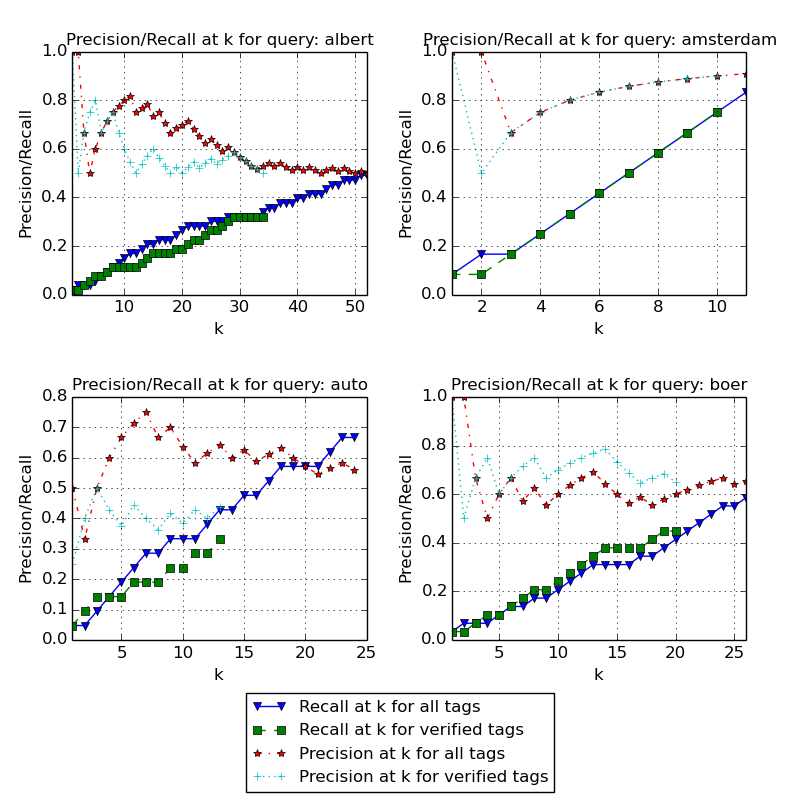
\includegraphics[scale=.55]{appendixa/queries1}
\end{figure}

\begin{figure}[H]
\centering
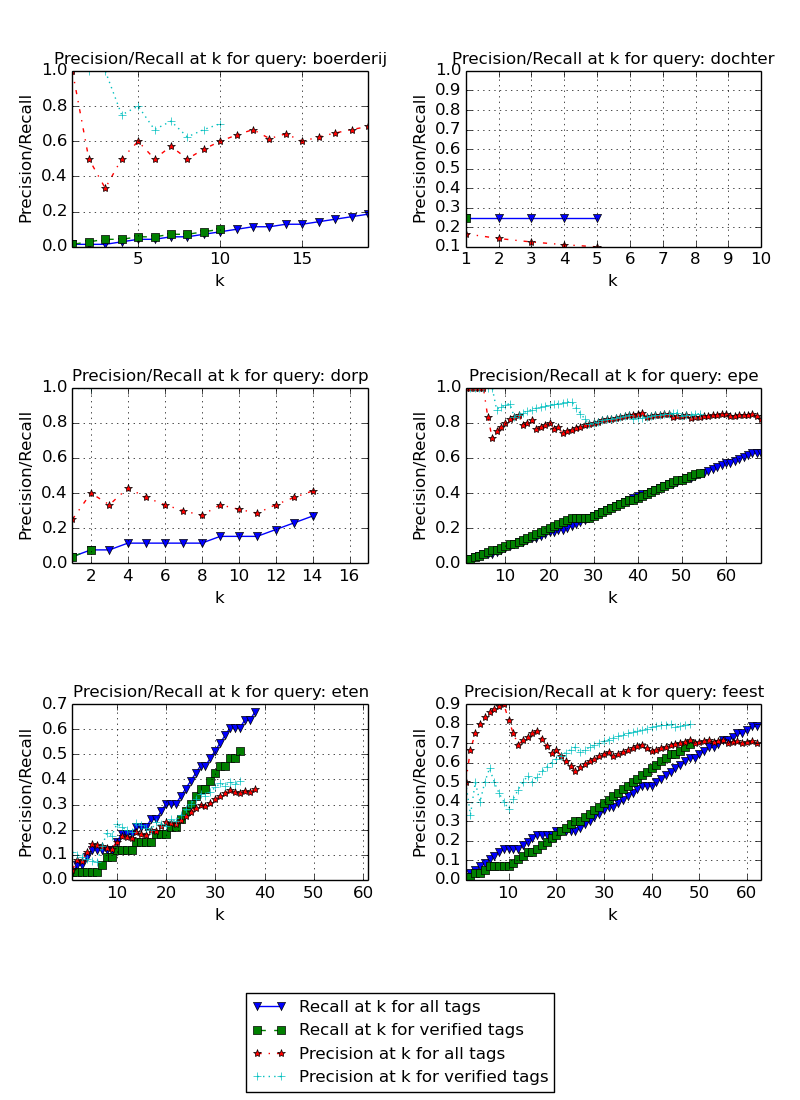
\includegraphics[width=\textwidth]{appendixa/queries5}
\end{figure}

\begin{figure}[H]
\centering
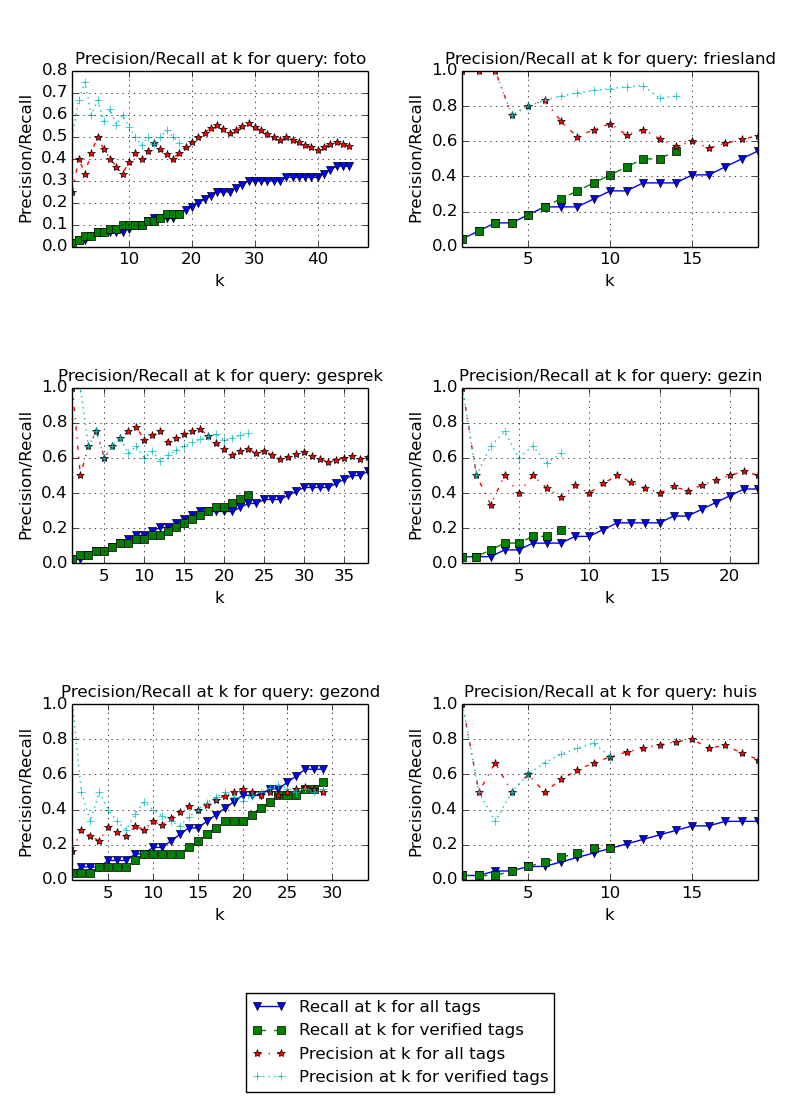
\includegraphics[width=\textwidth]{appendixa/queries13}
\end{figure}

\begin{figure}[H]
\centering
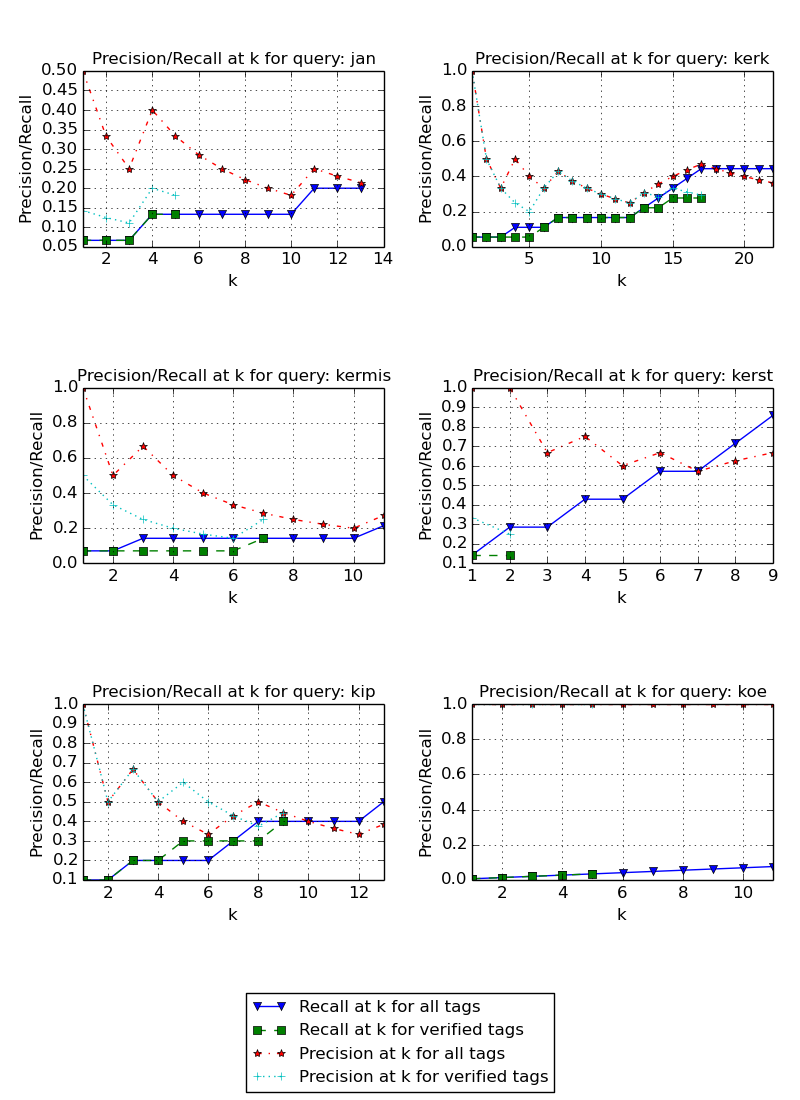
\includegraphics[width=\textwidth]{appendixa/queries19}
\end{figure}

\begin{figure}[H]
\centering
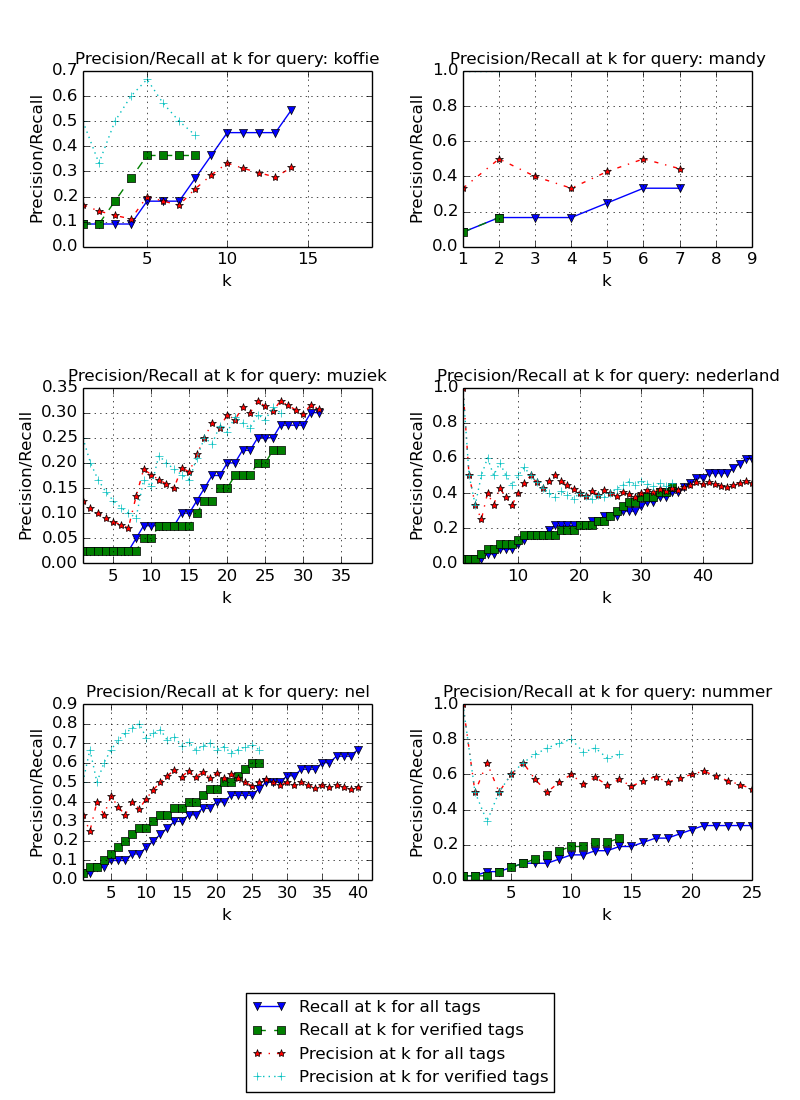
\includegraphics[width=\textwidth]{appendixa/queries25}
\end{figure}

\begin{figure}[H]
\centering
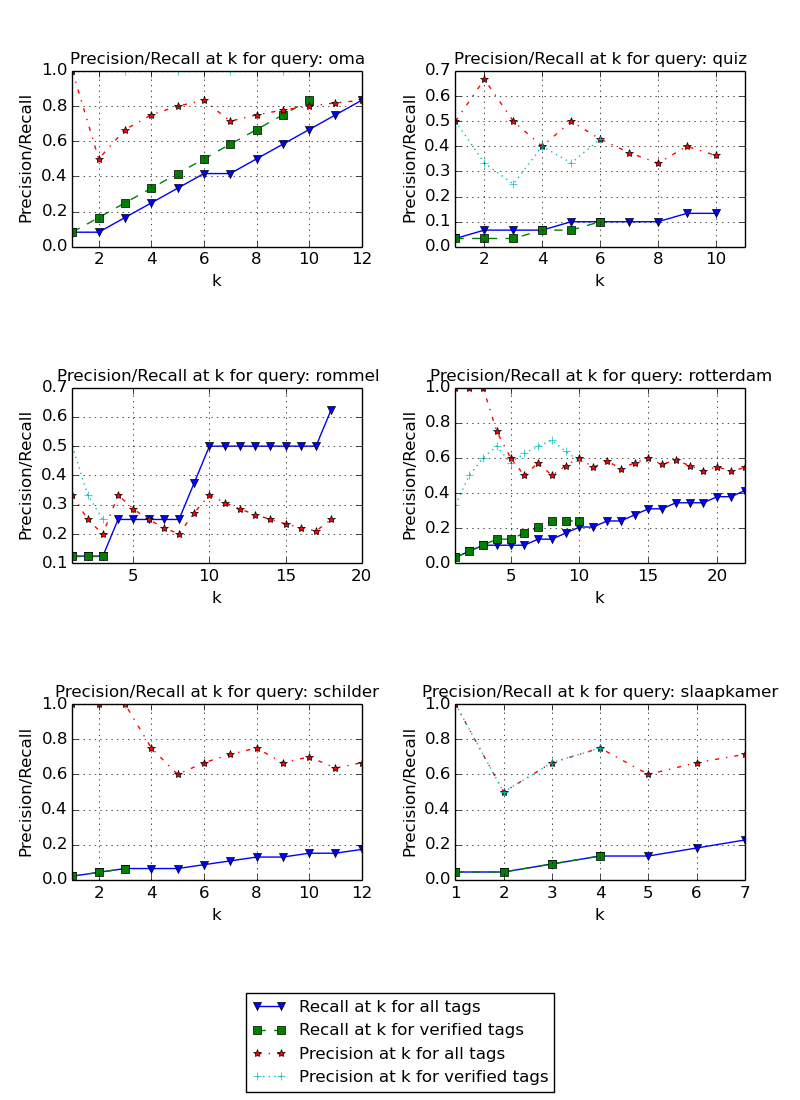
\includegraphics[width=\textwidth]{appendixa/queries31}
\end{figure}

\begin{figure}[H]
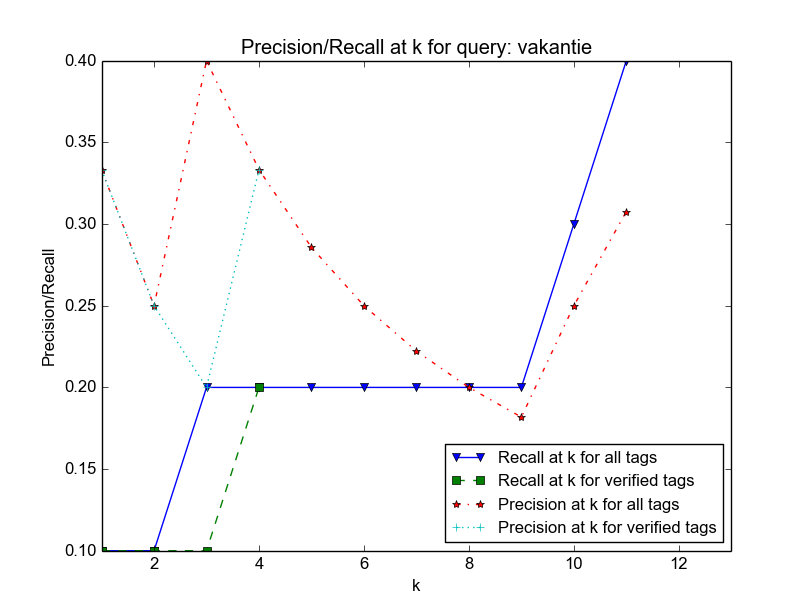
\includegraphics[width=\textwidth]{appendixa/queries43}
\end{figure}
\chapter{Query Precision over Time for Visual Search}\label{appen:precovertime}
This appendix shows how the precision metric for each query changed over time as more tags are acquired. The precision metric figures originate from the visual search study presented in Chap. \ref{chap:ecir}.

\begin{figure}[H]
\centering
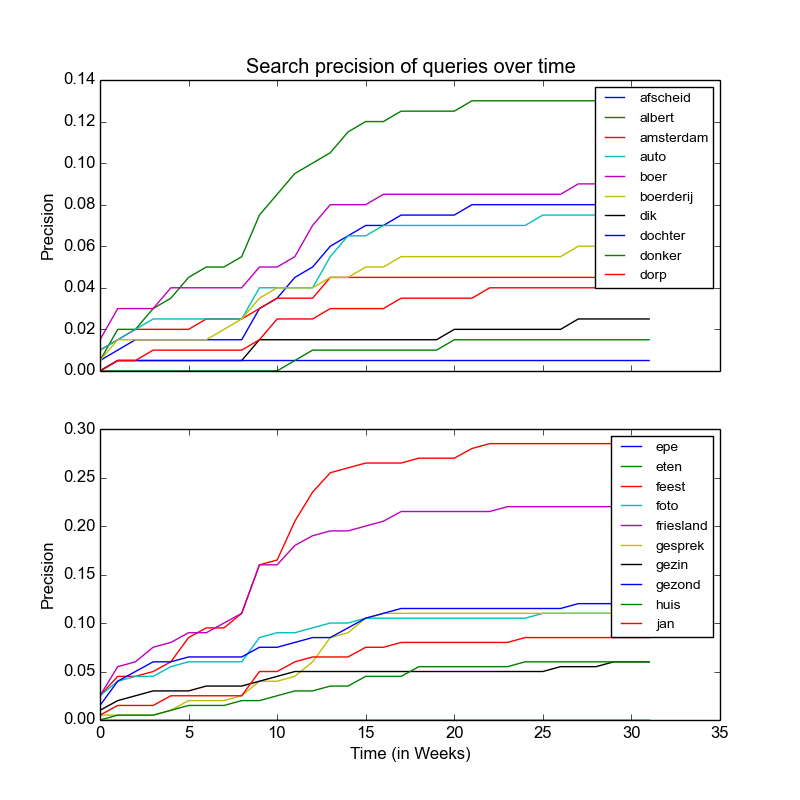
\includegraphics[scale=0.55]{appendixb/precisionovertime0}
\end{figure}


\begin{figure}[H]
\centering
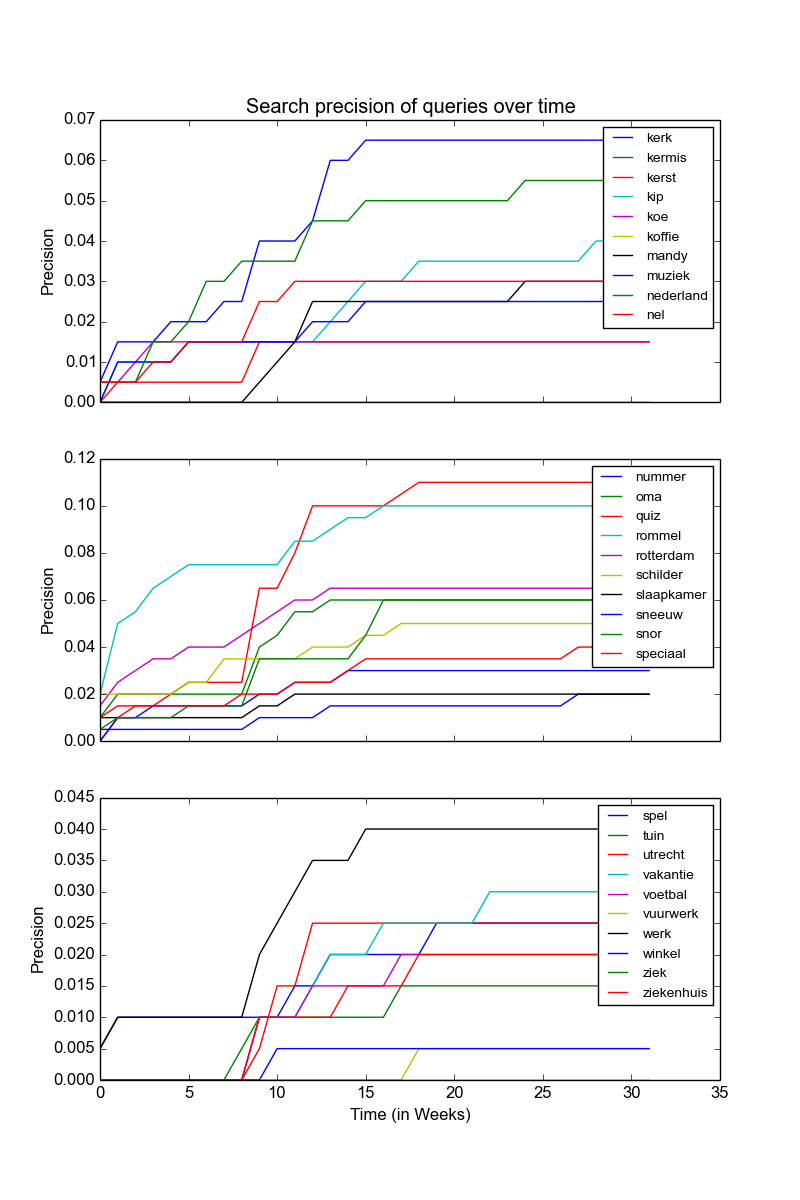
\includegraphics[width=\textwidth]{appendixb/precisionovertime20}
\end{figure}
\chapter{Query Recall over Time for Visual Search}\label{appen:recovertime}
This appendix shows how the precision metric for each query changed over time as more tags are acquired. The precision metric figures originate from the visual search study presented in Chap. \ref{chap:ecir}.

\begin{figure}[H]
\centering
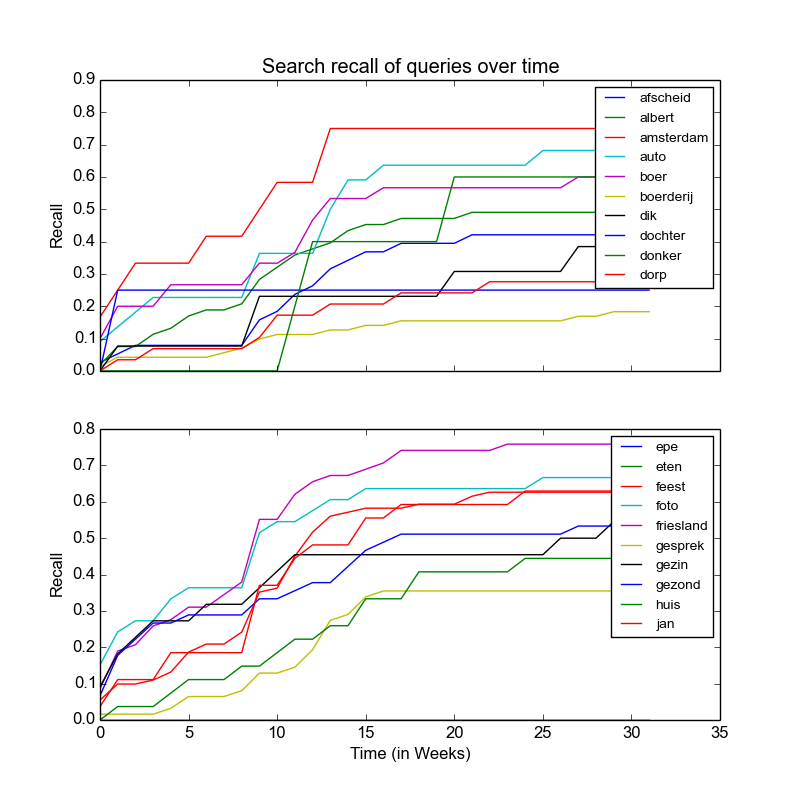
\includegraphics[scale=0.55]{appendixc/recallovertime0}
\end{figure}


\begin{figure}[H]
\centering
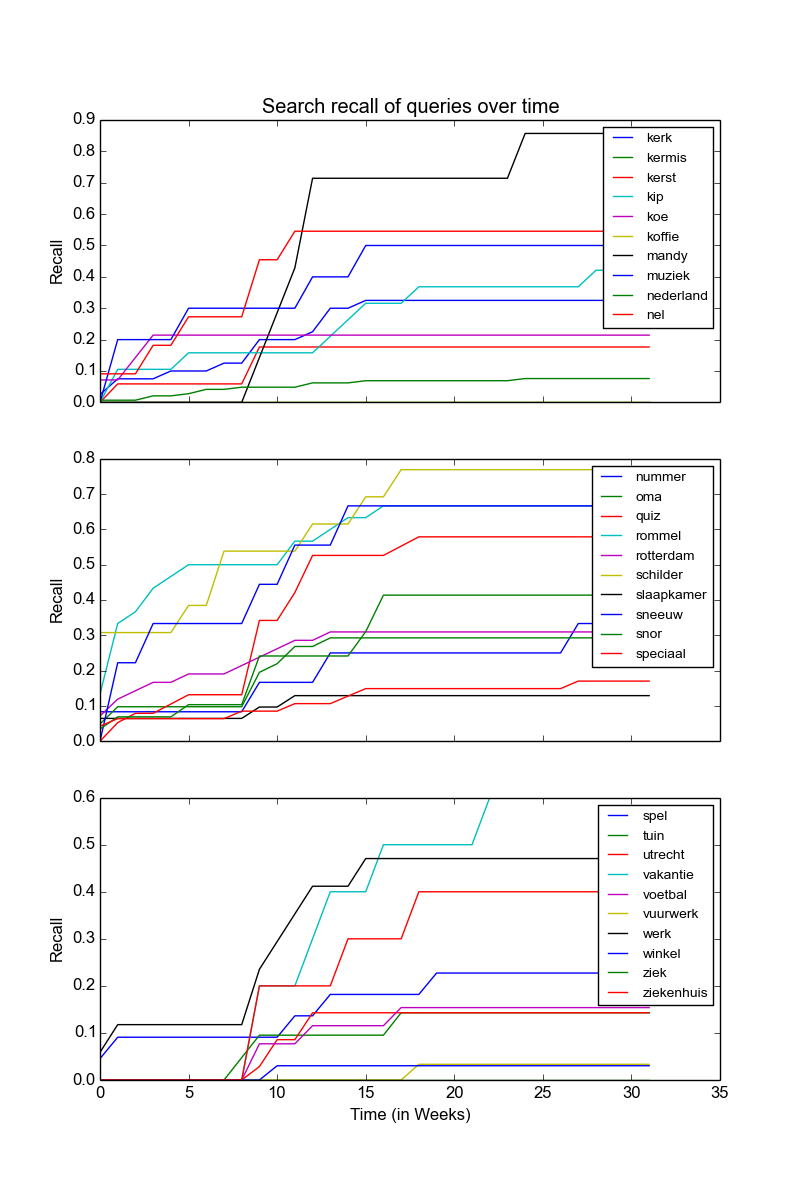
\includegraphics[width=\textwidth]{appendixc/recallovertime20}
\end{figure}
\chapter{Precision/Recall per Query for Topical Search}\label{appen:prec-recall-topical}
This appendix contains the detailed precision and recall metrics for each of the queries from the topical search study presented in Chap. \ref{chap:topicir-filter}. Note that the queries for which there were no results returned by the verified tags were left out.

\begin{figure}[H]
\centering
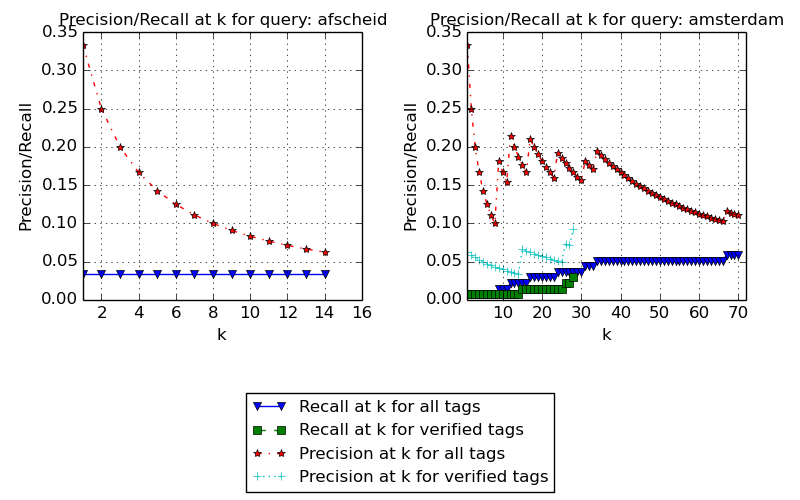
\includegraphics[scale=.55]{appendixd/queries-afscheid}
\end{figure}


\begin{figure}[H]
\centering
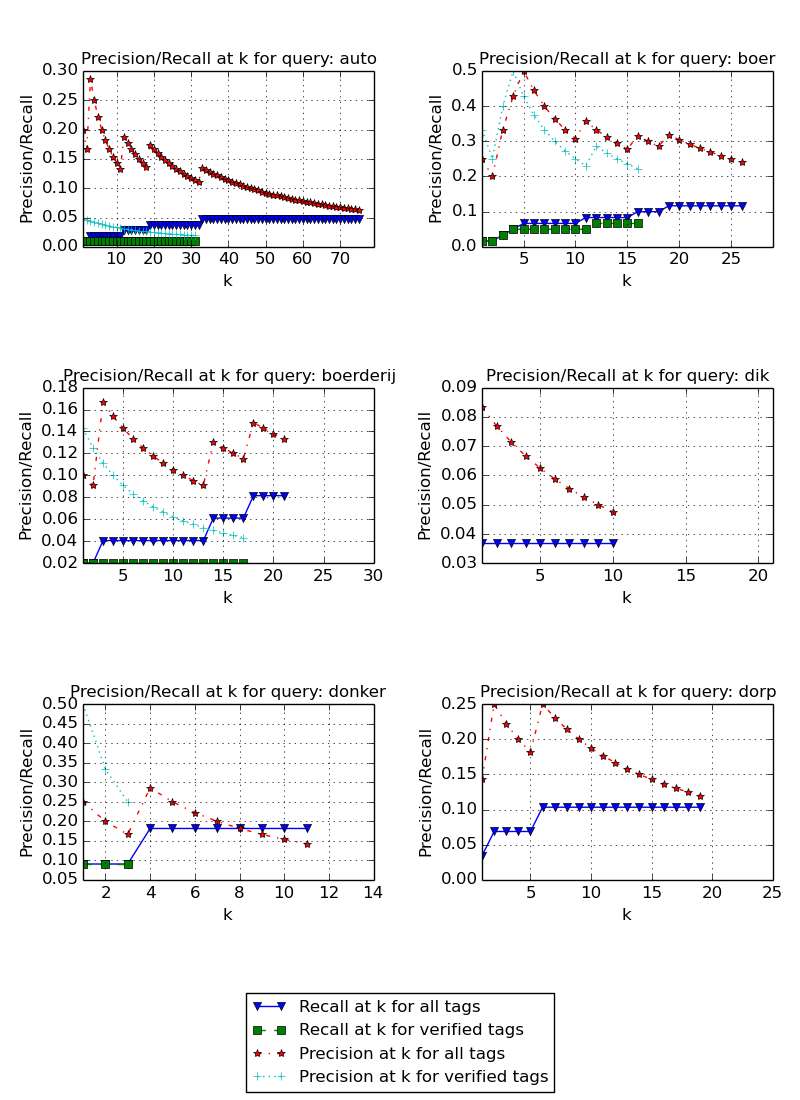
\includegraphics[width=\textwidth]{appendixd/queries-auto}
\end{figure}


\begin{figure}[H]
\centering
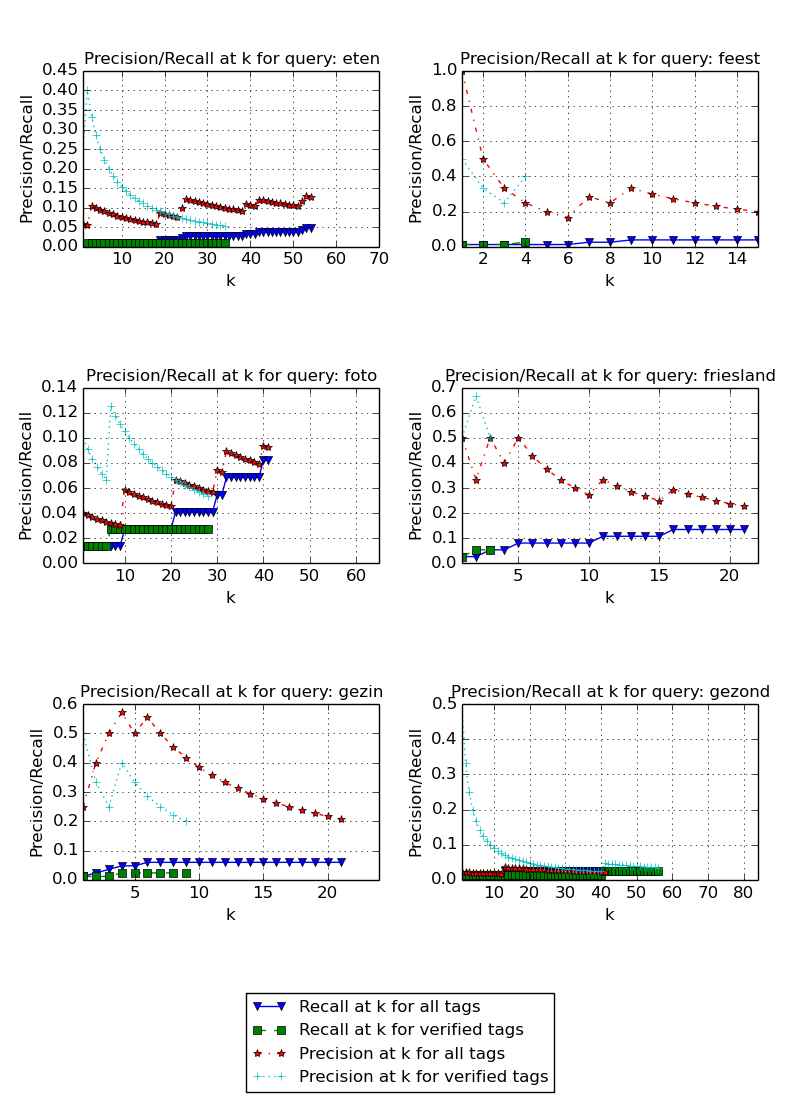
\includegraphics[width=\textwidth]{appendixd/queries-eten}
\end{figure}


\begin{figure}[H]
\centering
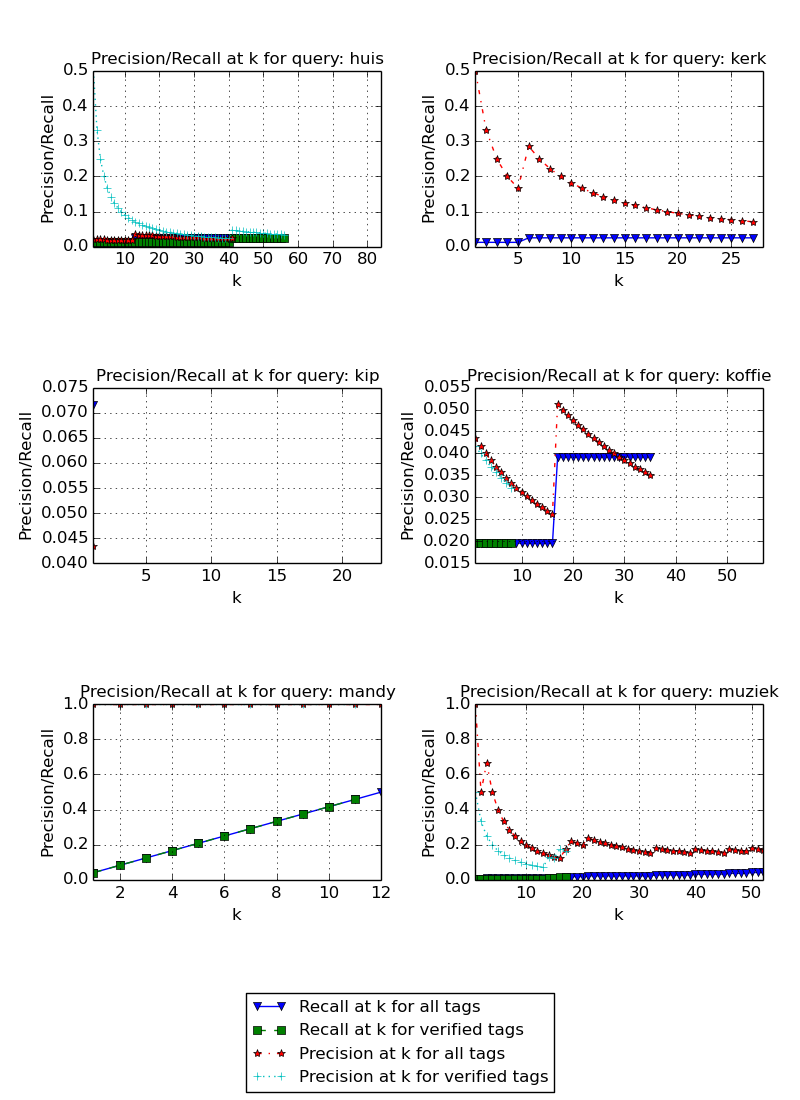
\includegraphics[width=\textwidth]{appendixd/queries-huis}
\end{figure}


\begin{figure}[H]
\centering
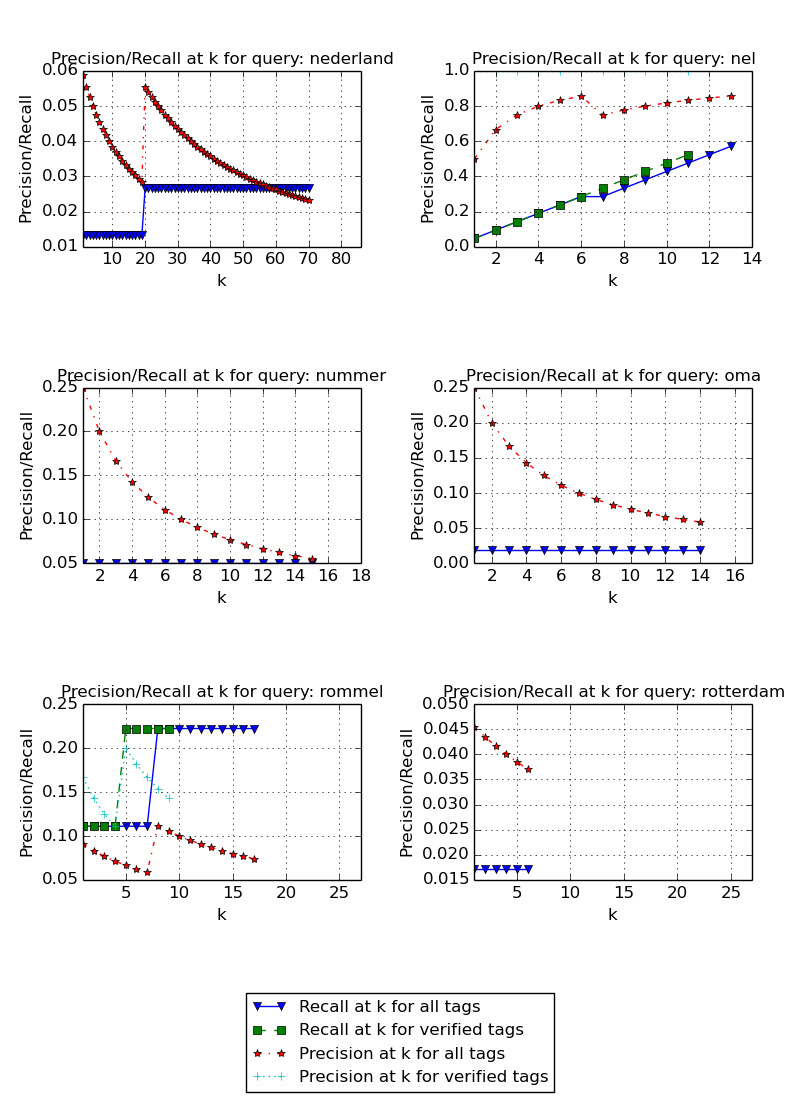
\includegraphics[width=\textwidth]{appendixd/queries-nederland}
\end{figure}


\begin{figure}[H]
\centering
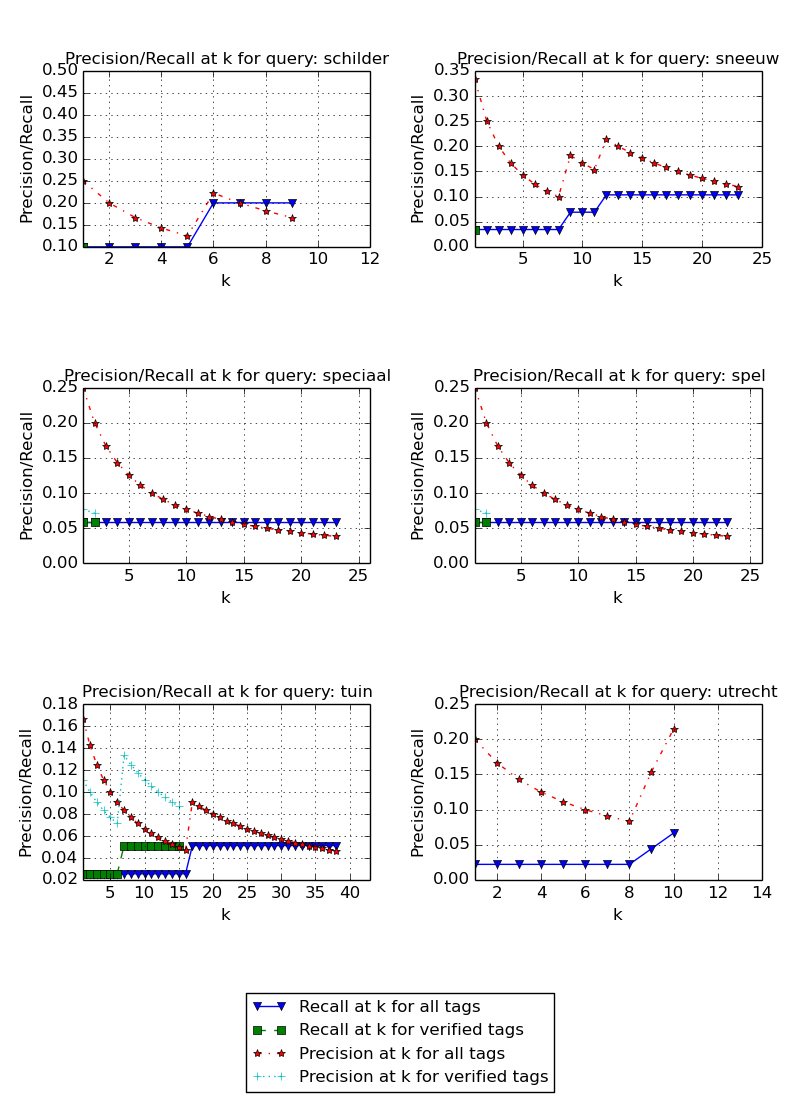
\includegraphics[width=\textwidth]{appendixd/queries-schilder}
\end{figure}


\begin{figure}[H]
\centering
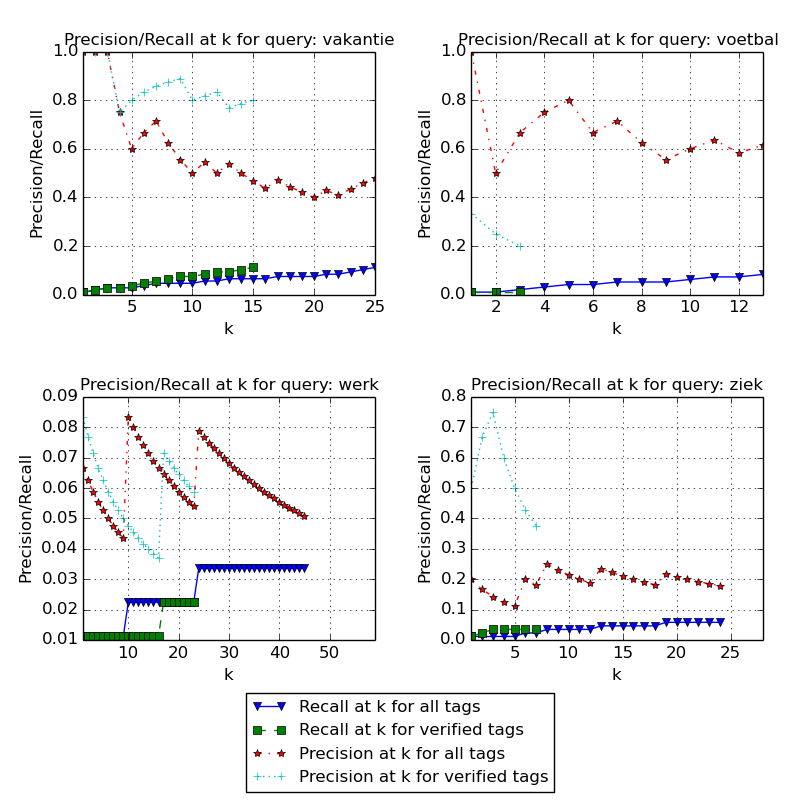
\includegraphics[width=\textwidth]{appendixd/queries-vakantie}
\end{figure}
\end{appendices}

\bibliographystyle{plain}
\bibliography{thesis}

\end{document}